\documentclass[onecolumn, letter paper]{report}

\usepackage{project}

\addbibresource{references.bib}

\begin{document}
\flushbottom
\maketitle

\chapter{Cartesian stiffness control}
The low level control of the hopping leg has been realized using PD control. Here, three functions have been implemented after \cite{di2020software}: A simple joint space PD controller with the control law:
\begin{equation}
    \pmb{\tau } =\pmb{\tau_{ff}} + \pmb{K_{p,j}}(\pmb{q_{des}} - \pmb{q}) + \pmb{K_{d,j}}(\pmb{\dot q_{des}} - \pmb{\dot q} ),
\end{equation}
Cartesian stiffness control, with the control law: 
\begin{equation}
    \pmb{\tau} = \pmb{J^T} (\pmb{f_{ff}} + \pmb{K_{p,c}}(\pmb{p_{des}} - \pmb{p}) + \pmb{K_{d,c}}(\pmb{\dot p_{des}} - \pmb{\dot p} )),
\end{equation}
and combined stiffness control, which combines the two controllers from above:
\begin{equation}
    \pmb{\tau} = \pmb{\tau_{ff}} + \pmb{K_{p,j}}(\pmb{q_{des}} - \pmb{q}) + \pmb{K_{d,j}}(\pmb{\dot q_{des}} - \pmb{\dot q} ) + \pmb{J^T} (\pmb{f_{ff}} + \pmb{K_{p,c}}(\pmb{p_{des}} - \pmb{p}) + \pmb{K_{d,c}}(\pmb{\dot p_{des}} - \pmb{\dot p} )).
\end{equation}
$\pmb{\tau}$ denotes here the motor torque vector, $\pmb{\tau_{ff}}$ the commanded feed forward torques, $\pmb{K_{p,j}}$ and $\pmb{K_{d,j}}$ the joint space gain matrices, $\pmb{K_{p,c}}$ and $\pmb{K_{d,c}}$ the Cartesian space gain matrices, $\pmb{J}$ the hybrid Jacobian at the end effector and $\pmb{f_{ff}}$ the feed forward force in Cartesian space. The current and desired joint positions  are given with $\pmb{q}$ and $\pmb{q_{des}}$ in joint space, and the actual and desired end effector position vectors are written as $\pmb{p}$ and $\pmb{p_{des}}$. 

\section{Parameter tuning}
The mentioned low level controllers require quite a few parameters to be tuned. Here, we see some differences between the tuning of the real system and tuning the simulation, therefore they have to be tuned individually.
For the real system, the joint level control is likely to be done by the motor internal PD controller, as it is more stable. Therefore, it is recommended to just use the Cartesian stiffness control and tune the joint space gains separately in the internal motor controller. In simulation, there might be no internal motor  controller. Therefore, the combined stiffness can be used.

When tuning the gains, one has to consider that higher joint level gains reduce the influence of the Cartesian stiffness and vice-versa. To stabilize the joint positions and counteract vibrations, larger joint space gains are more likely to give good results. For effectively applying some Cartesian feed forward forces instead, or to apply different stiffnesses in x and y direction, low joint level gains are required, since they can neutralize the feed forward forces otherwise. 




% Here we can tune the stiffness and damping in Cartesian coordinates. As a rule of thumb, the $K_p$ value should be around 50 times larger than $K_d$. Now it is important to observe the system carefully adapt the gains until the required behaviour is reached. As 


\chapter{Hopping control}
Hopping can be simplified with the Spring Loaded Inverted Pendulum (SLIP) model, in which a mass is mounted on a massless spring \cite{Tedrake}. Due to this spring, the energy in the system stays constant. By adding or removing energy into the system, e.g., by applying some force to the spring, the jumping height can be controlled.

Since our hopping leg is designed to have lightweight legs, it is similar to a SLIP model. The main difference is, that our hopping leg has no inbuilt elasticity. Therefore, it has to apply the desired jumping energy during every lift-off. To achieve this, two controllers have been implemented on top of a state machine. The state machine divides the jumping cycle into 3 (or 4) phases with different goals:  In the flight phase, the leg prepares its position for the touchdown. In the real system, this flight phase is divided into two phases, flight ascend and flight, since the contact detection does not work reliable. During the flight phase, the leg is stiff, since it has to reach a specific position. The flight phase ends with the first contact of the  leg with the ground. During the touchdown, the movement of the leg is damped, since its energy cannot be used due to the absence of elastic elements. When the downwards movement is fully stopped, the lift-off phase starts. The conditions for the phase transitions are written in \autoref{tab:conditions} more precisely.
The two implemented control approaches both use this lift-off phase, to apply the desired energy for the next jump. In \autoref{fig:state} you can see the phase diagrams of the state machine used in the real system and in simulation.

\begin{table}[htb!]
    \centering
    \caption{Phase transition conditions for the state machine in the real system and in simulation.}
    \begin{tabular}{lc|c}
        \textbf{Phase to enter}&\textbf{Real system}&\textbf{Simulation}  \\ \hline
         Touchdown & ($|\tau_1| \geq 10$ or $|\tau_2| \geq 10$) and $x \leq x_{des}-0.005$ & contact \\
         Lift-off & $|\pmb{\dot p}| < 0.1$ and $x \leq x_{des}$   & $\dot x \geq 0$\\
         Flight ascend & $x \geq x_{des} + 0.16$ & -- \\
         Flight &  not ($|\tau_1| \geq 10$ or $|\tau_2| \geq 10$) & no contact
    \end{tabular}
    \label{tab:conditions}
\end{table}

\begin{figure}[htb!]
    \centering
    \begin{subfigure}[b]{.49 \textwidth}
    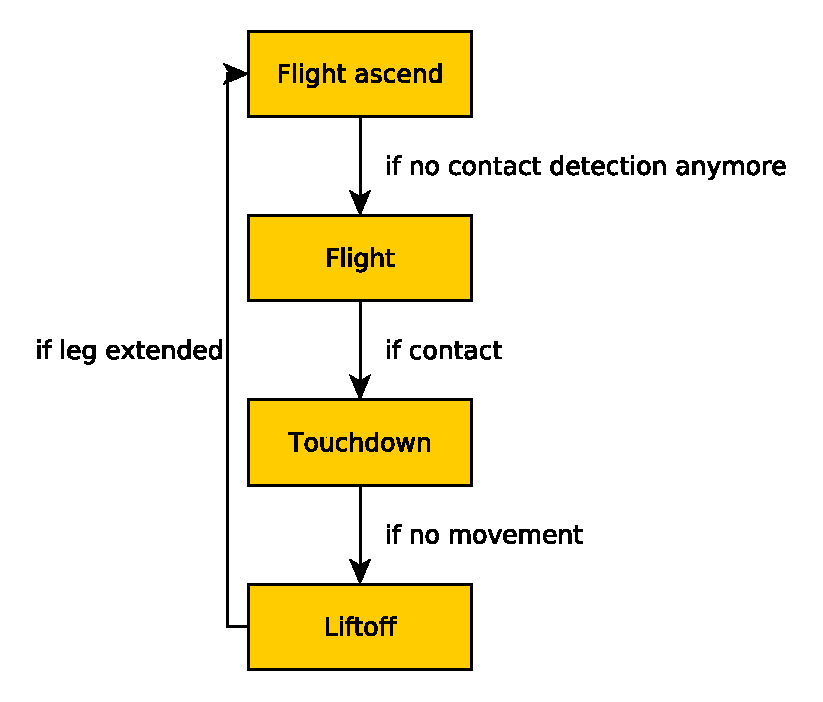
\includegraphics[width=\textwidth]{figures/phase_diagram_real_system.pdf}
    \subcaption{Real system}
    \end{subfigure}
    \begin{subfigure}[b]{.49 \textwidth}
    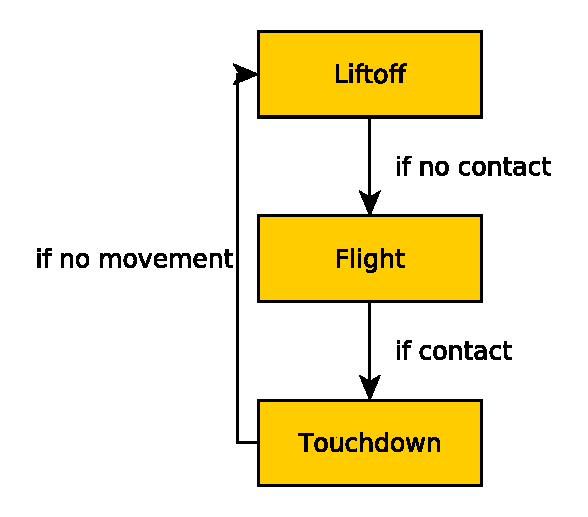
\includegraphics[width=.7\textwidth]{figures/phase_diagram_simulation.pdf}
    \vspace{1cm}
    \subcaption{Simulation}
    \end{subfigure}
    \caption{Phase diagrams of the state machine for the real system (a) and the simulation (b). }
    \label{fig:state}
\end{figure}

\section{Gain scheduling control}
The gain scheduling control uses Cartesian stiffness control to mirror the behaviour of the spring in the SLIP model. For this, a high stiffness is necessary to reapply sufficient energy into the system. To be able to lift-off and to counteract dissipation, the desired leg length during the lift-off phase can be increased and/or a feed forward force can be applied.



\section{Energy shaping control}
The advantage of energy shaping control is, that we can control the jumping height by applying energy to the system until the desired energy $E_{des}$, which is needed to jump at a desired height $h_{des}$, is reached.
With the simplification, that we assume all mass $m$ in the shoulder of the jumping leg the desired energy can be calculated with:
\begin{equation}
    E_{des} = m g h_{des},
\end{equation}
where g is the gravitational acceleration. Since  the hopping is one dimensional in the current setup, only the kinetic energy in this direction (x-direction, see \autoref{fig:leg}) will be used for further calculations.

\begin{figure}[htb!]
    \centering
    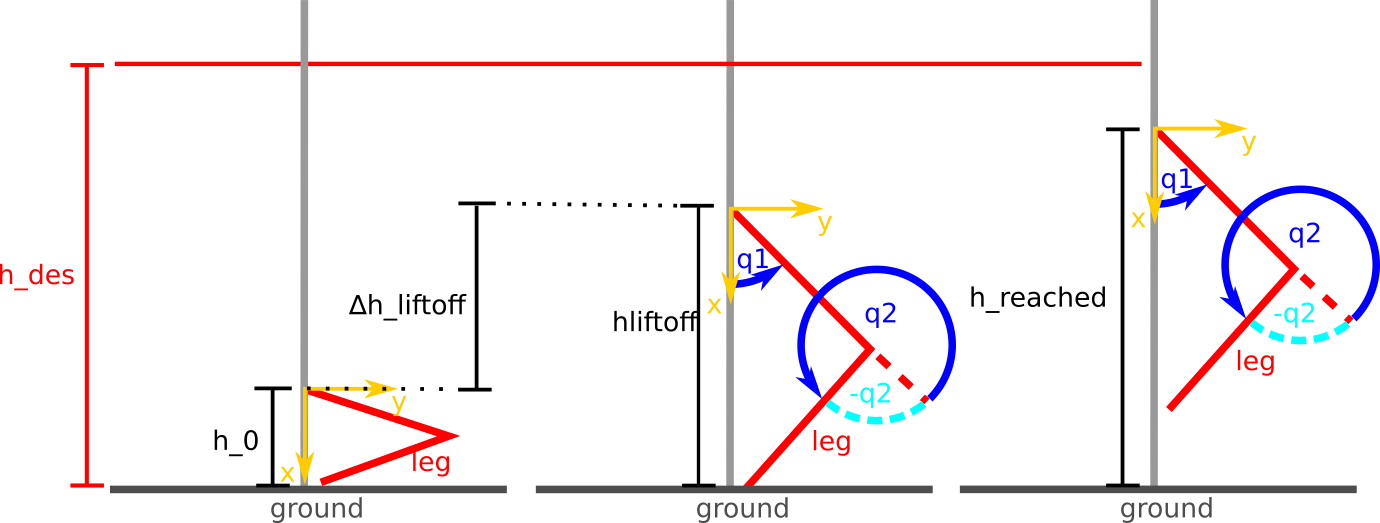
\includegraphics[width=\textwidth]{figures/hopping_leg_seq.png}
    \caption{Schematic diagram of the hopping leg and the used parameters.}
    \label{fig:leg}
\end{figure}

% For energy shaping control, two different approaches have been tried. 
% \subsection{Non-continuous energy shaping}
The used approach is non-continuous energy shaping, where we just observe the reached energy, which is: 
\begin{equation}
    E = m g h_{reached}
\end{equation}

For reaching this energy, we had to apply a feed forward force $F_{ff}$ during the lift-off phase. 
The needed force $F_e$ is almost constant and can be estimated as
\begin{equation}
    F_e = \frac{m g (h_{des}-h_{0})}{\Delta h_{lift-off}},
\end{equation}
where $h_{0}$ is the base position at the start of the lift-off phase and $\Delta h_{lift-off}$ is the distance, over which the leg has ground contact, and hence can apply force.

Since the applied feed forward force is proportional to the reached energy, we can write:
\begin{equation}
    E \propto k F_e
\end{equation}
and hence:
\begin{equation}
    \dot E \propto \dot k F_e
\end{equation}

Thus, we can add energy to the system by increasing $k$ and remove energy by decreasing it. To control $k$ the following update rule can be used:
\begin{equation}
    k_{i+1} = k_{i}  (\frac{E_{des}}{E})^2
\end{equation}

  

% \subsection{Lift-off energy shaping}
% As a second approach, energy shaping has been used during lift-off to shape the feed forward force until the desired kinetic energy is reached. In this approach, its use is quite similar to energy shaping in a single pendulum swing up. The main difference is, that we cannot pump energy into the system, again, due to the missing elasticity. Hence, the whole energy has to be applied in just one “swing up”.

% Since the legs were assumed to play a minor role in the energy of the system, for simplification the energy of the system has been assumed as:
% \begin{equation}
% \label{energy}
%     E = \frac{1}{2}\, m\, \dot q_0^2 + m \,g\, q_0,
% \end{equation}
% with the derivative
% \begin{equation}
% \label{eq:Edot}
%     \dot E = m \, \dot q_0 \, \ddot q_0 + m \, g \, \dot q_0.
% \end{equation}

% In the hopping leg, the acceleration $\ddot q_0$ is almost only controllable with contact forces, which can be used as feed forward force in x direction $F_{ffx}$ in the Cartesian stiffness control. The resulting joint acceleration is given by \autoref{eq:acc}:
% \begin{equation}
%     \label{eq:acc}
%     \ddot q_0 = \frac{F_{ffx}}{m} - g
% \end{equation}
% Hence, the derivative of the energy in the system  can be written as:
% \begin{equation}
% \label{Edot}
%     \dot E = F_{ffx} \, \dot q_0
% \end{equation}
% % In \autoref{eq:Edot} we see, that we can add


% When we now define the difference between the current energy and the  desired energy $\widetilde{E} = E - E_{des}$ we see, that we have still the same derivative:
% \begin{equation}
%     \dot{ \widetilde{E}} = \dot E = F_{ffx} \dot q_0
% \end{equation}


\chapter{State estimation}
For the energy shaping control, a height feedback is necessary. Therefore, a simple state estimation has been implemented. Since during the flight phase no additional forces can be applied to the system, we can expect the acceleration to be $g$. As we know the lift-off position and velocity, we can calculate the current height of the base $h$ with:
% \begin{equation}
% \begin{aligned}
%     g =& \frac{dv}{dt} \\
%     \int_{t_0}^t g \, dt=& \int_{v_0}^v \,dv\\
    
% \end{aligned}
% \end{equation}
\begin{equation}
    h = \frac{1}{2} g (t^2 - t_0^2) - g t_0 (t - t_0) + v_0 (t - t_0) + h_0,
\end{equation}
where $t$ is the current time and  $t_0$ is the time at lift-off. $h_0$ and  $v_0$ denote the height and  velocity of the base at time $t_0$.

This simple state estimator, which is only used during flight phase, since with ground contact forward kinematics are more accurate, gives us quite good results. Nevertheless, we still have to admit that it ignores friction and dynamic effects of the leg movements.

\chapter{Increasing the jumping height}
\label{sec:increasingheight}
During our trials on the real system, we found that we are limited to around 0.5 m jumping height when we just apply feedforward forces in x-direction (see \autoref{fig:leg}).
We can find the reason for this behaviour in the way, how the torques are calculated from the feed forward forces, as \autoref{eq:fff} always leads to zero torques in the shoulder joint, when the end effector position as well as the feed forward force is zero in y-direction. 
\begin{equation}
\label{eq:fff}
    \pmb{\tau} = \pmb{J^T} \pmb{f_{ff}}
\end{equation}
Thus, just one motor applies torques during the lift-off.
To use the full potential of both motors, we have to apply some feedforward forces within the friction cone in y-direction (see \autoref{fig:leg}) too. 
Using heuristics, we found a feed forward force of 15 N in y-direction to be beneficial for the jumping height. In further research, the optimal feed forward force distribution can be found using optimal control. 


\chapter{Backflip control in simulation}
For the energy shaping control, a support to do flips has been implemented too. For these backflips, a trajectory has been added to the original desired hip joint angle $q_1$ during flight phase. Additionally, the joint positions had to be corrected by adding $n\cdot 2\pi$, where $n$ is the number of forward flips minus the number of backflips. This added values are updated directly before the flying phase, where a flip  will happen. Hence, the trajectory of the flip is cancelling out this difference in the beginning of the flip.
For a backflip, the new joint position $q_{1,t}$ is defined with:
\begin{equation}
    q_{1,t} = q_1 - 2 \pi + (-\pi \cos(\frac{\pi t}{\Delta t_{i-1} - t_s}) + \pi),
\end{equation}
where $t$ is the time since the flip started, $\Delta t_{i-1}$ is the duration of the last flight phase and $t_s$ is a safety time, which was set to 0.1 s.
For a forward flip, the expression was accordingly:
\begin{equation}
    q_{1,t} = q_1 + 2 \pi - (-\pi \cos(\frac{\pi t}{\Delta t_{i-1} - t_s}) + \pi).
\end{equation}

Additionally, flips with a change of the knee direction have been implemented. For a backflip, the expression for the hip joint position was:
\begin{equation}
    q_{1,t} = -q_1 - 2 \pi + (-(|q1| + \pi) \cos(\frac{\pi t}{\Delta t_{i-1} - t_s}) + \pi),
\end{equation}
and for a forward flip:
\begin{equation}
    q_{1,t} = -q_1 - 2 \pi - (-(|q1| + \pi) \cos(\frac{\pi t}{\Delta t_{i-1} - t_s}) + \pi).
\end{equation}
At the same time, the position of the knee joint $q_2$ has been updated for both flip directions with:
\begin{equation}
    q_{2,t} = - q_2 \cos(\frac{\pi t}{\Delta t_{i-1} - t_s})
\end{equation}


To use these backflips, a list has been used to define arbitrary sequences of normal jumps and forward- and backflips, were always the next element is given to a prepare function, which adds or subtracts $2 \pi$ to the current adjustment term and saves the new knee direction for inverse kinematics. Afterwards, the jumping mode is performed during flight phase.   

\section{Backflip in the real system}
In the real system, a backflip has been performed as well. This has been done much easier, by just commanding the current hip joint position plus $2 \pi$ during the flight phase. Afterwards, the script stopped.
In future, a similar approach to the simulation would be interesting.
% \newpage
\chapter{Results}


\section{Hopping control in simulation}
% For simulation, energy shaping control has been implemented inclusive backflip support. This backflip support adds a trajectory to the current desired state and can follow arbitrary sequences of backflips, forward flips and normal jumps.
The simulation was able to get close to the desired height values of 0.4 m, 0.5 m and 0.6 m as plotted in \autoref{fig:simheight}.
But since the state recognition in simulation is worse than in the real system, the desired height cannot always be reached correctly. But in previous tests, using not the estimated but the real state, the simulation was able to maintain desired height quite stable.
In \autoref{fig:simsequence4}, \ref{fig:simsequence5} and \ref{fig:simsequence6} exemplary jumping sequences of the 3 desired heights are plotted.

\begin{figure}[htb!]
    \centering
    \begin{subfigure}{.49\textwidth}
    \centering
    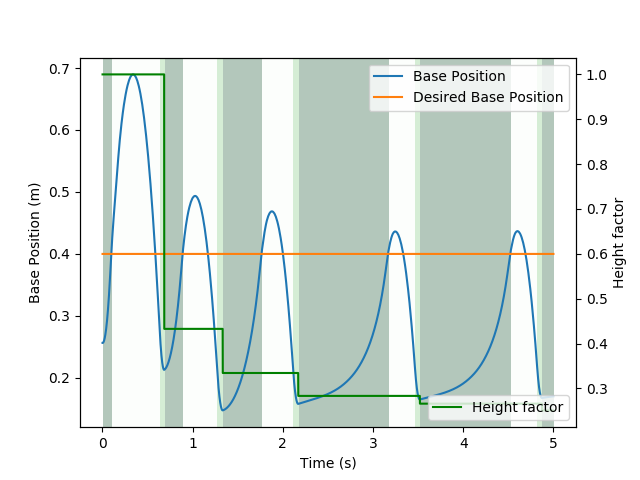
\includegraphics[width=\textwidth]{figures/sim0.4m/base_position.png}
    \subcaption{Desired jumping height: 0.4 m}
    \end{subfigure}
    \begin{subfigure}{.49\textwidth}
    \centering
    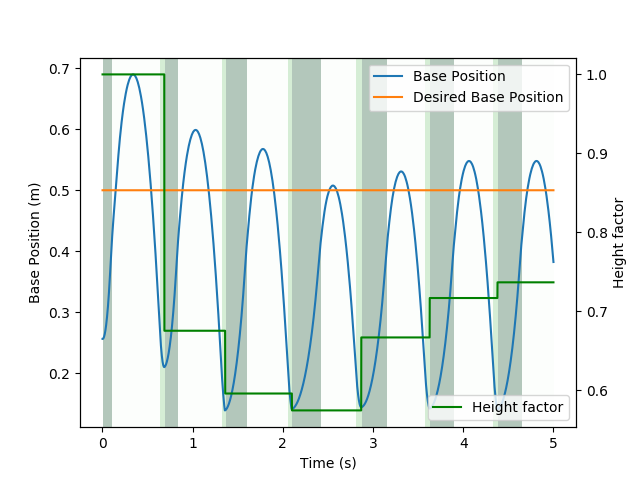
\includegraphics[width=\textwidth]{figures/sim0.5m/base_position.png}
    \subcaption{Desired jumping height: 0.5 m}
    \end{subfigure}
    \begin{subfigure}{.49\textwidth}
    \centering
    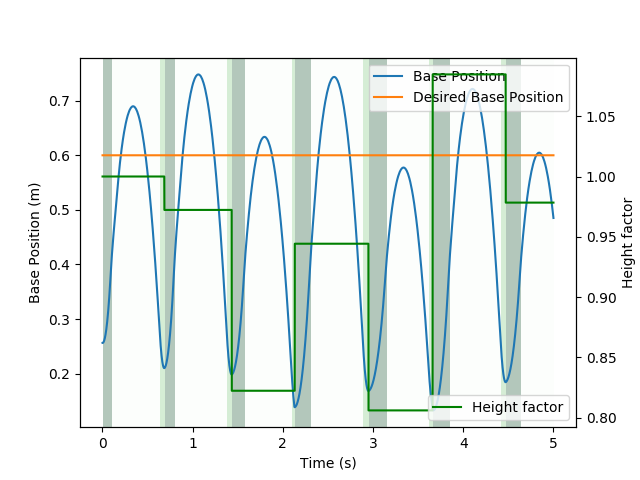
\includegraphics[width=\textwidth]{figures/sim0.6m/base_position.png}
    \subcaption{Desired jumping height: 0.6 m}
    \end{subfigure}
    \caption{Jumping heights with energy shaping control and a desired height of 0.4 m (a), 0.5 m (b) and 0.6 m (c) (yellow line) in simulation. The background colour indicates the current phase of the state machine. The flight phase is white, the touchdown phase is light green and the lift-off phase has a dark green background colour.}
    \label{fig:simheight}
\end{figure}
\begin{figure}[htb!]
    \centering
    \begin{subfigure}{.24\textwidth}
    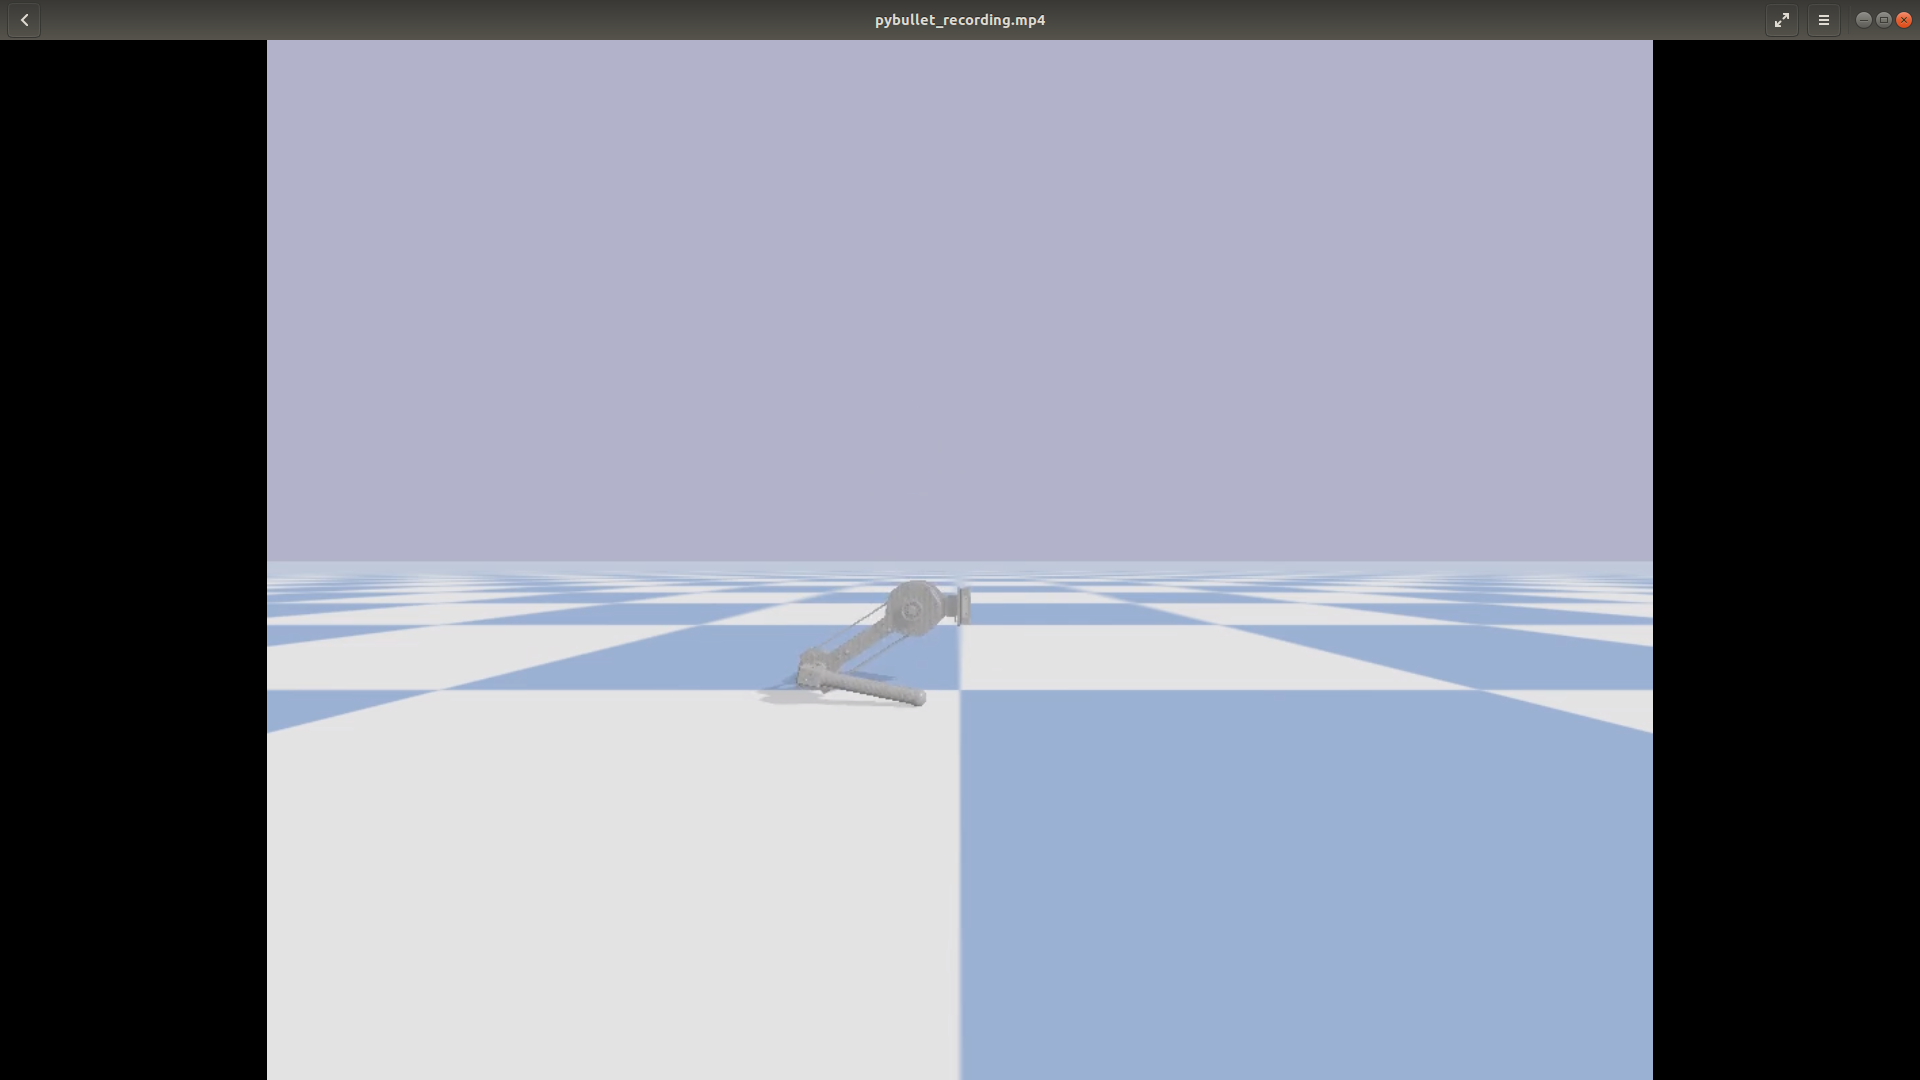
\includegraphics[width=\textwidth, trim={25cm 10cm 25cm 5cm}, clip]{figures/sim0.4m/s41.png}
    \end{subfigure}
    \begin{subfigure}{.24\textwidth}
    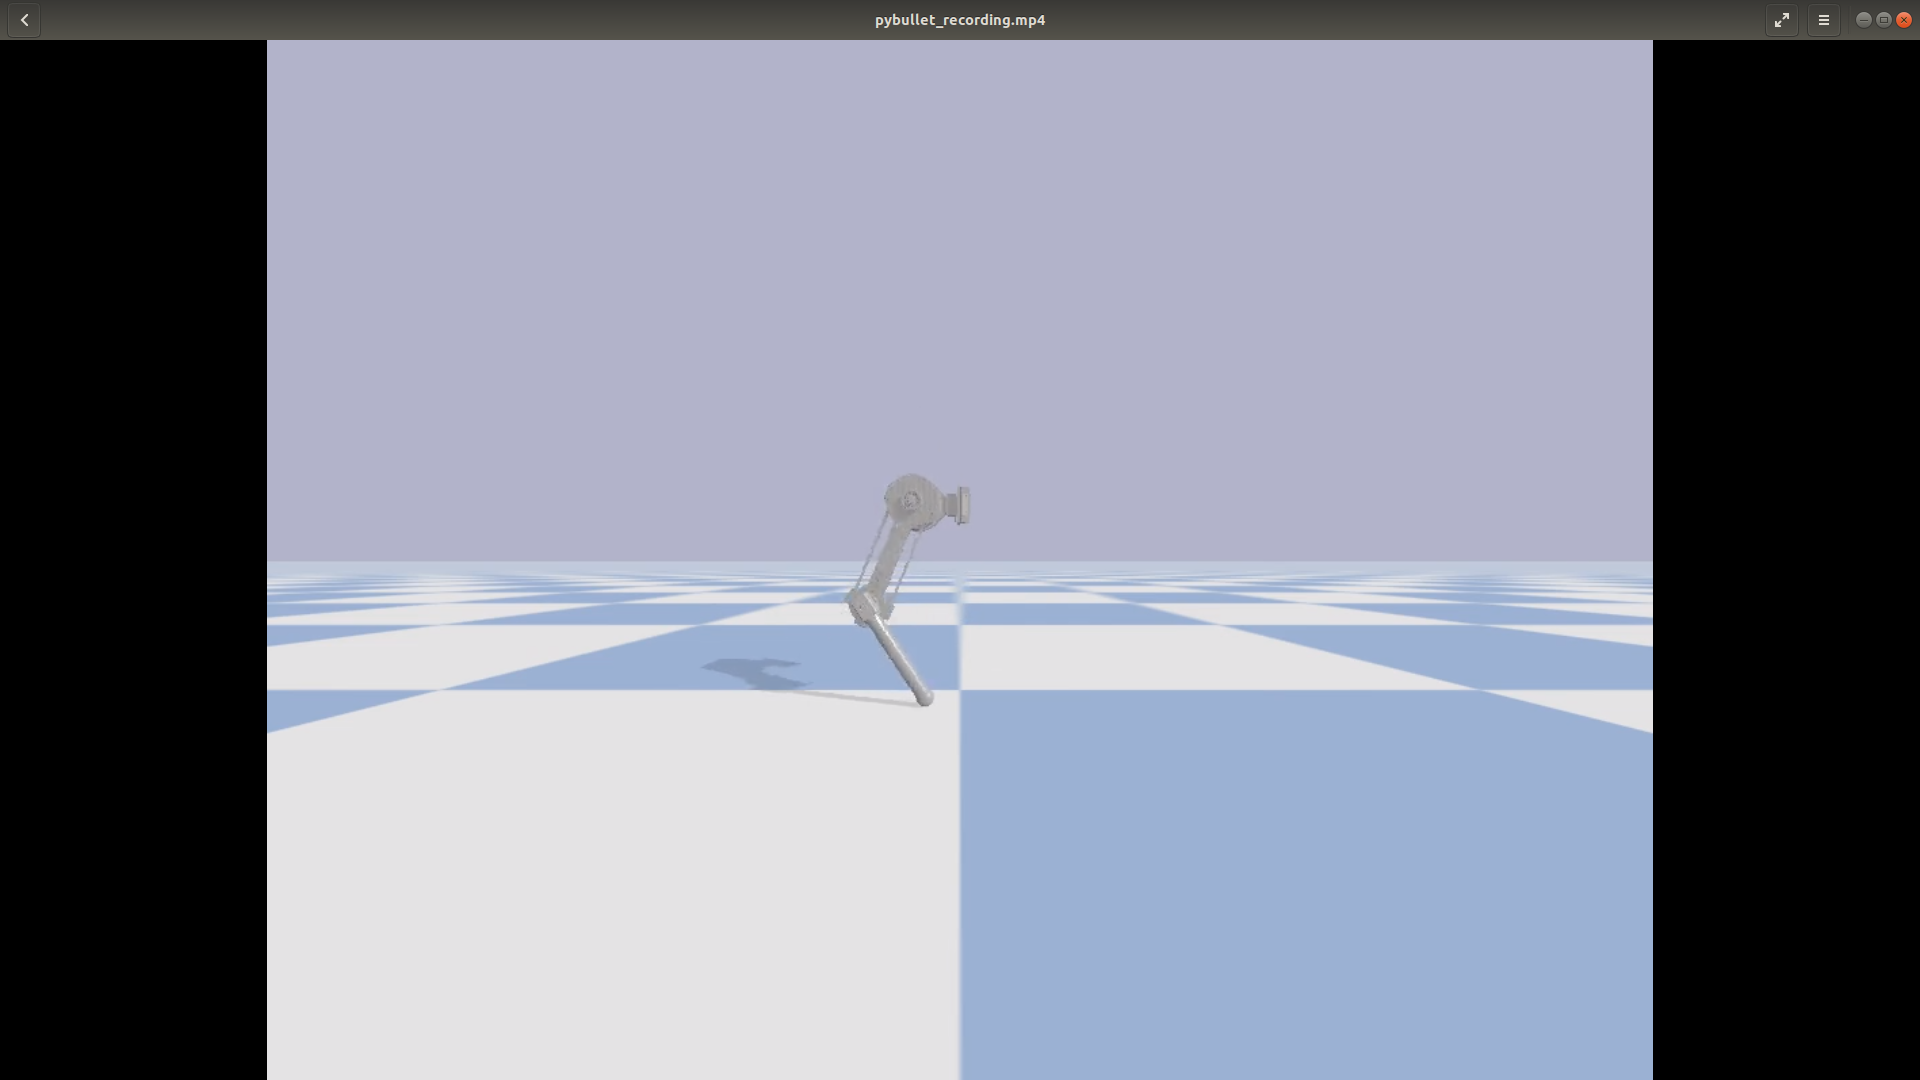
\includegraphics[width=\textwidth, trim={25cm 10cm 25cm 5cm}, clip]{figures/sim0.4m/s42.png}
    \end{subfigure}
    \begin{subfigure}{.24\textwidth}
    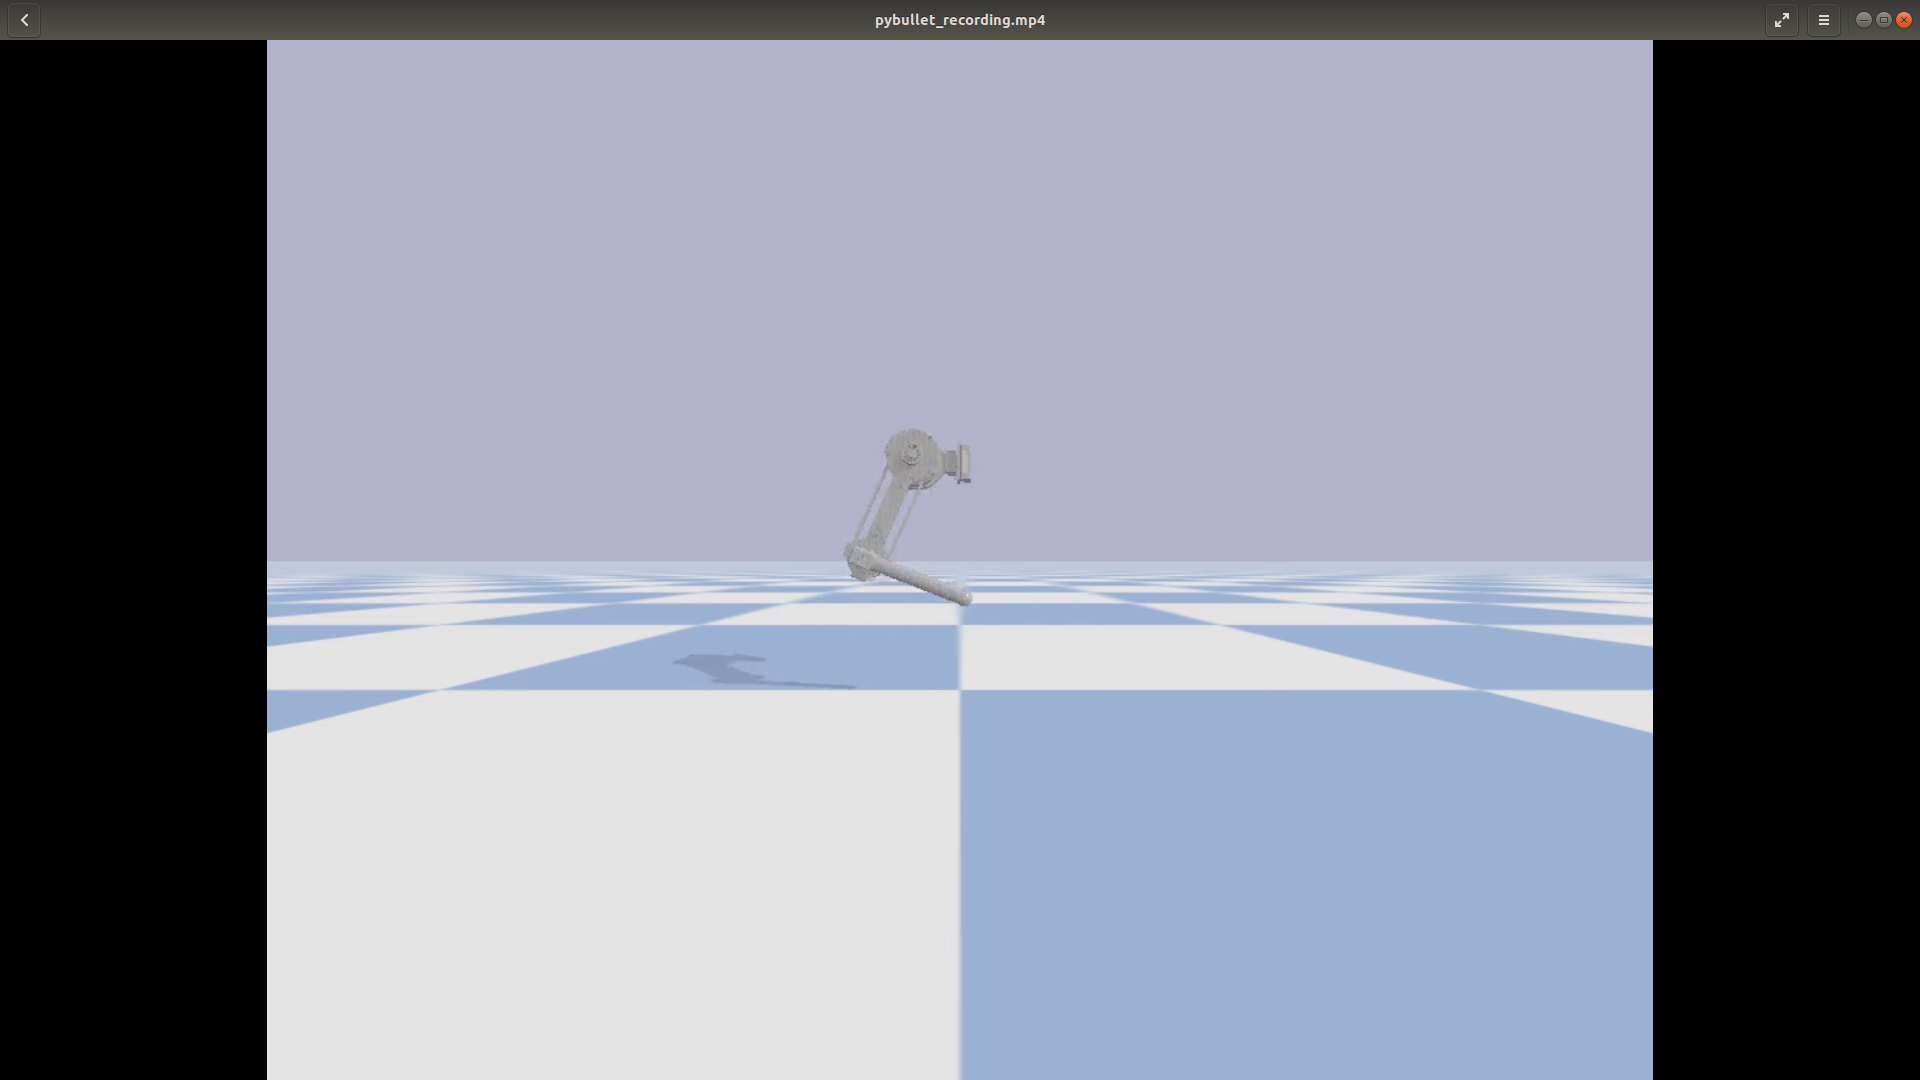
\includegraphics[width=\textwidth, trim={25cm 10cm 25cm 5cm}, clip]{figures/sim0.4m/s43.png}
    \end{subfigure}
    \begin{subfigure}{.24\textwidth}
    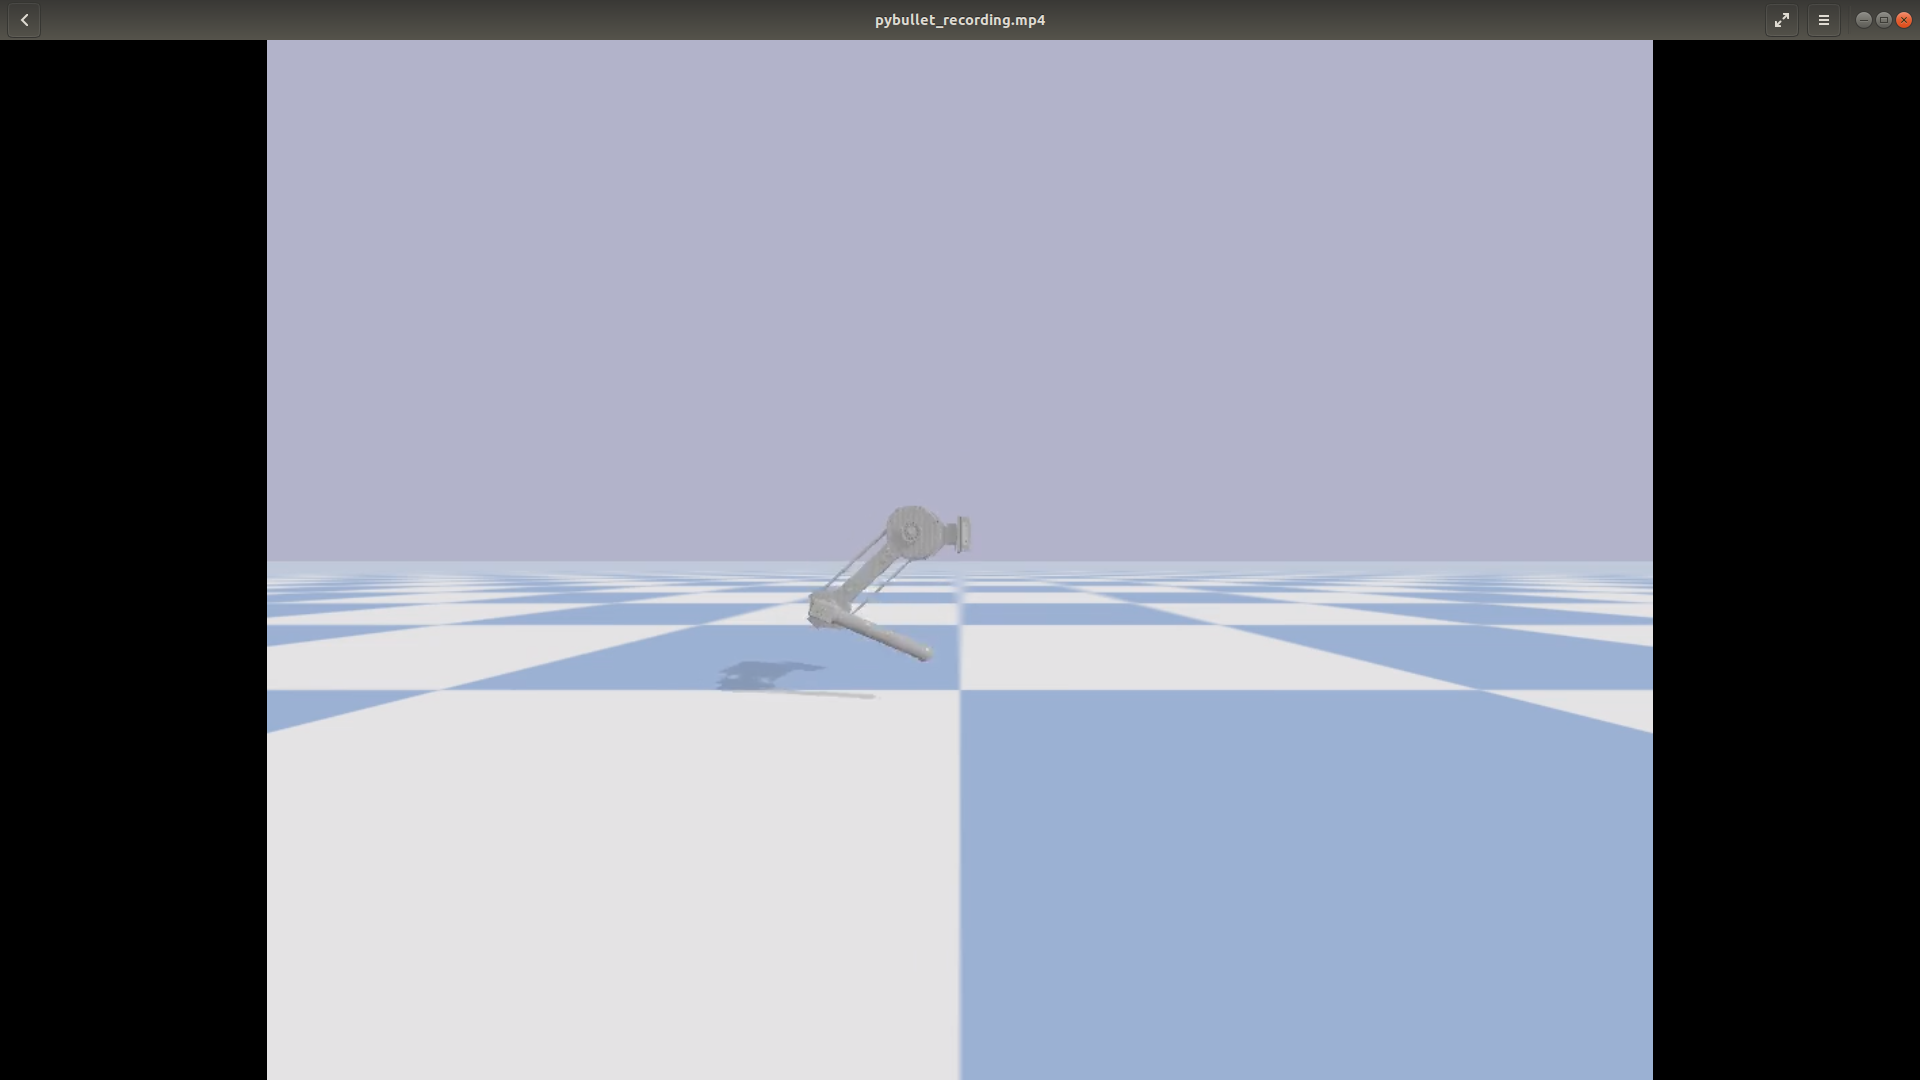
\includegraphics[width=\textwidth, trim={25cm 10cm 25cm 5cm}, clip]{figures/sim0.4m/s44.png}
    \end{subfigure}
    \caption{Simulated jumping sequence for 0.4 m desired height}
    \label{fig:simsequence4}
\end{figure}
\begin{figure}[htb!]
    \centering
    \begin{subfigure}{.24\textwidth}
    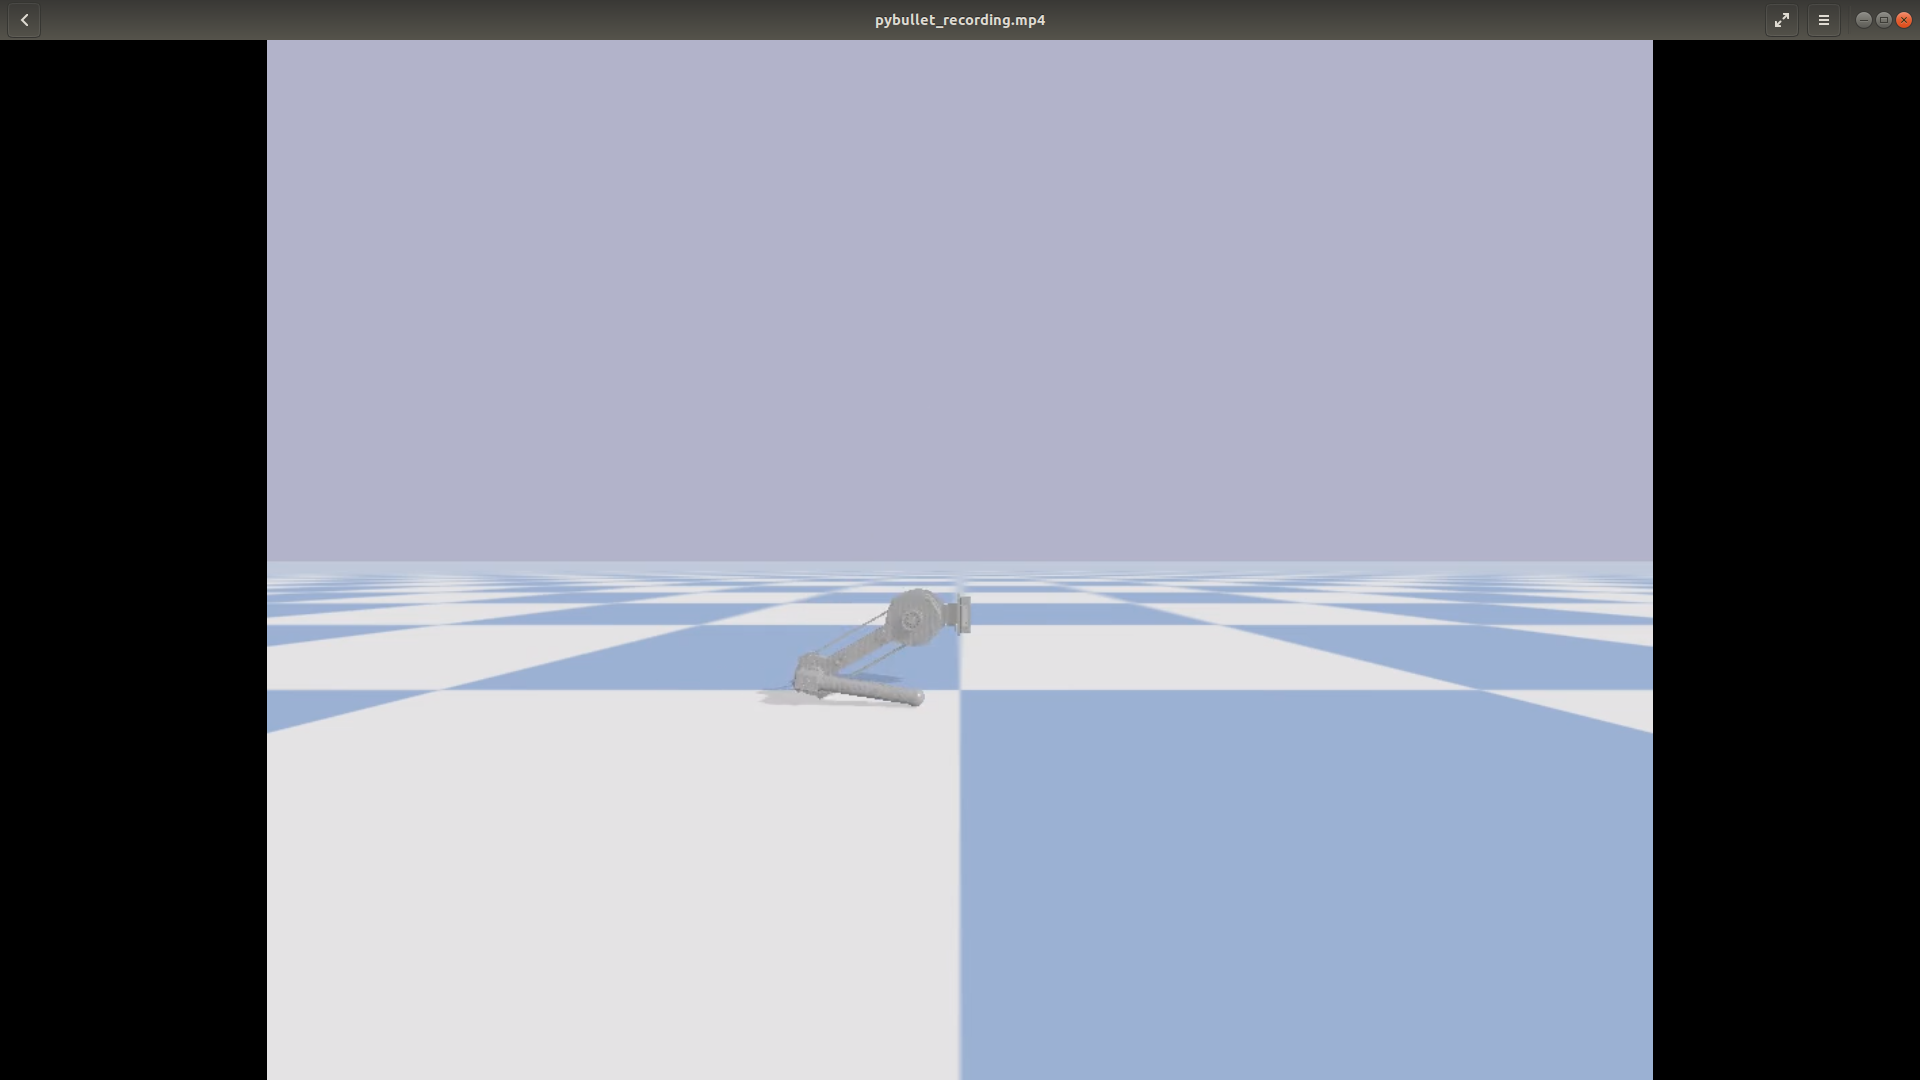
\includegraphics[width=\textwidth, trim={25cm 10cm 25cm 5cm}, clip]{figures/sim0.5m/s51.png}
    \end{subfigure}
    \begin{subfigure}{.24\textwidth}
    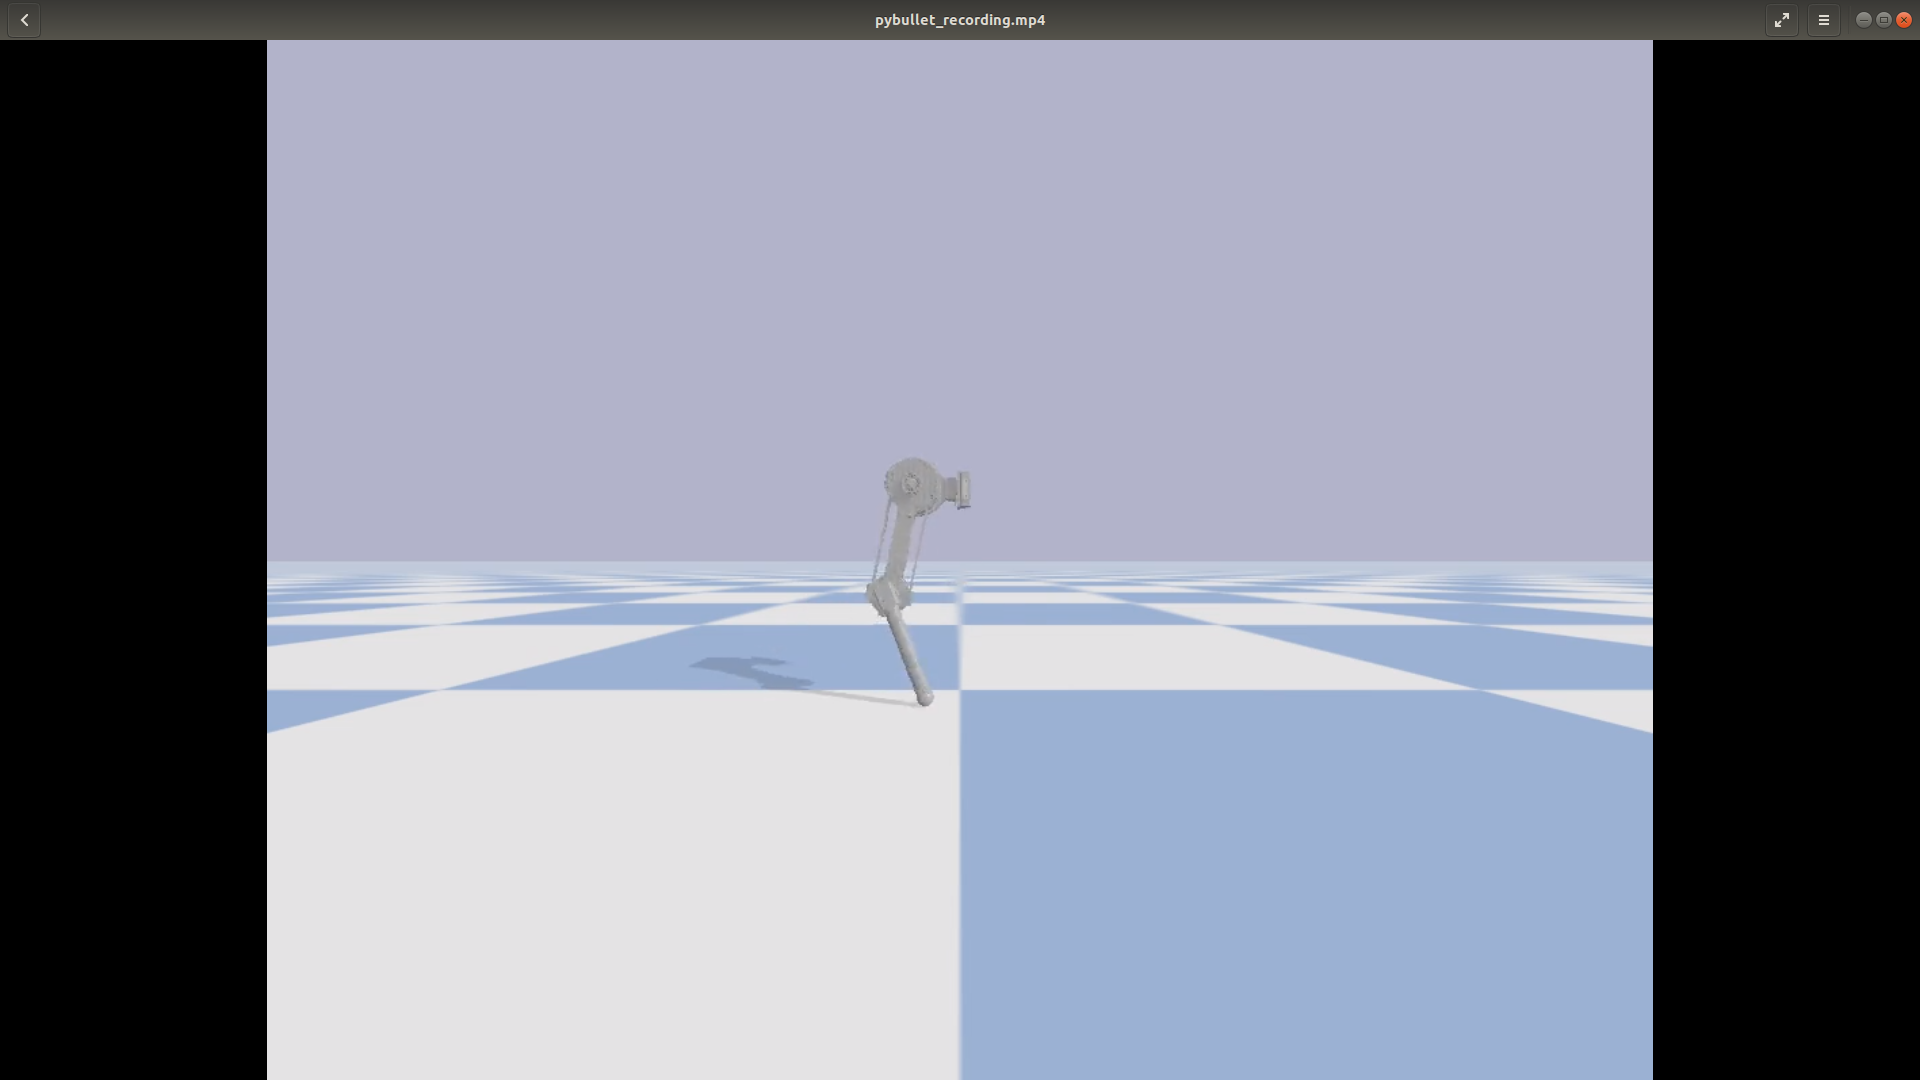
\includegraphics[width=\textwidth, trim={25cm 10cm 25cm 5cm}, clip]{figures/sim0.5m/s52.png}
    \end{subfigure}
    \begin{subfigure}{.24\textwidth}
    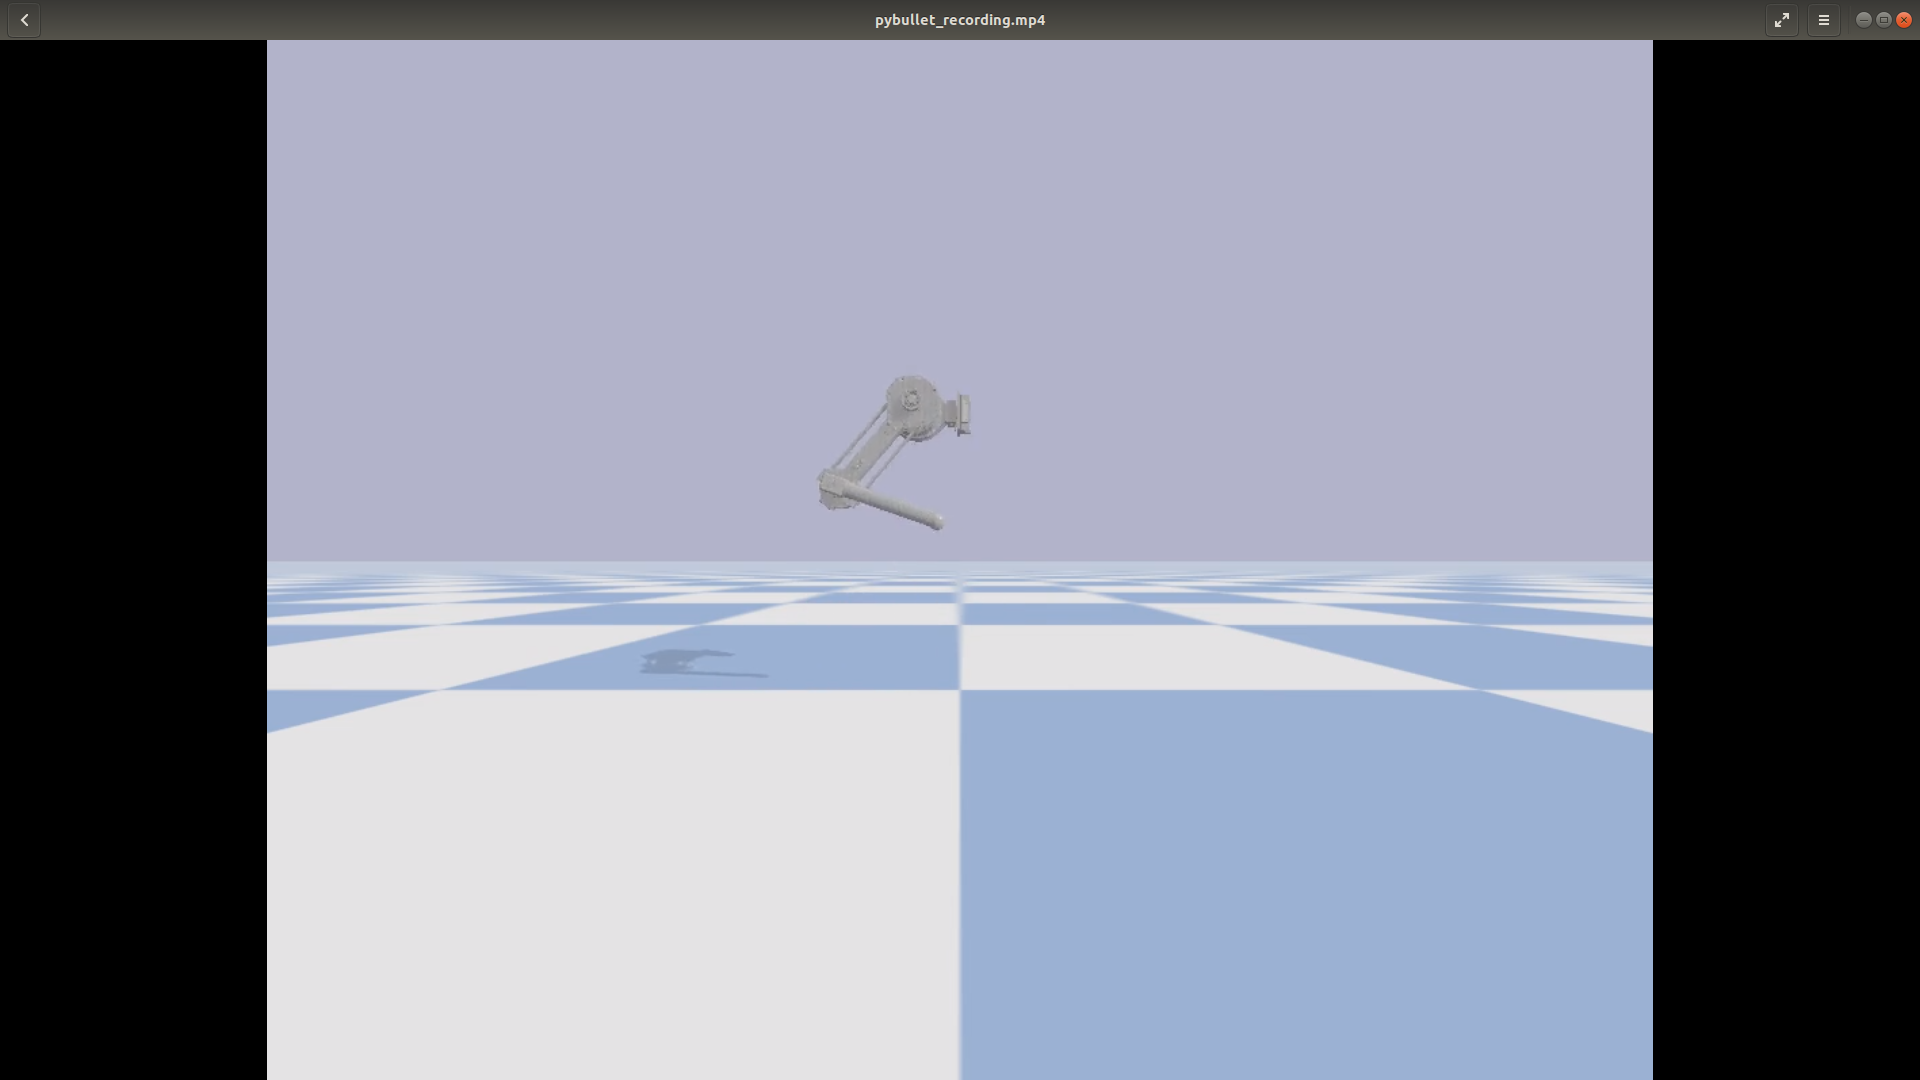
\includegraphics[width=\textwidth, trim={25cm 10cm 25cm 5cm}, clip]{figures/sim0.5m/s53.png}
    \end{subfigure}
    \begin{subfigure}{.24\textwidth}
    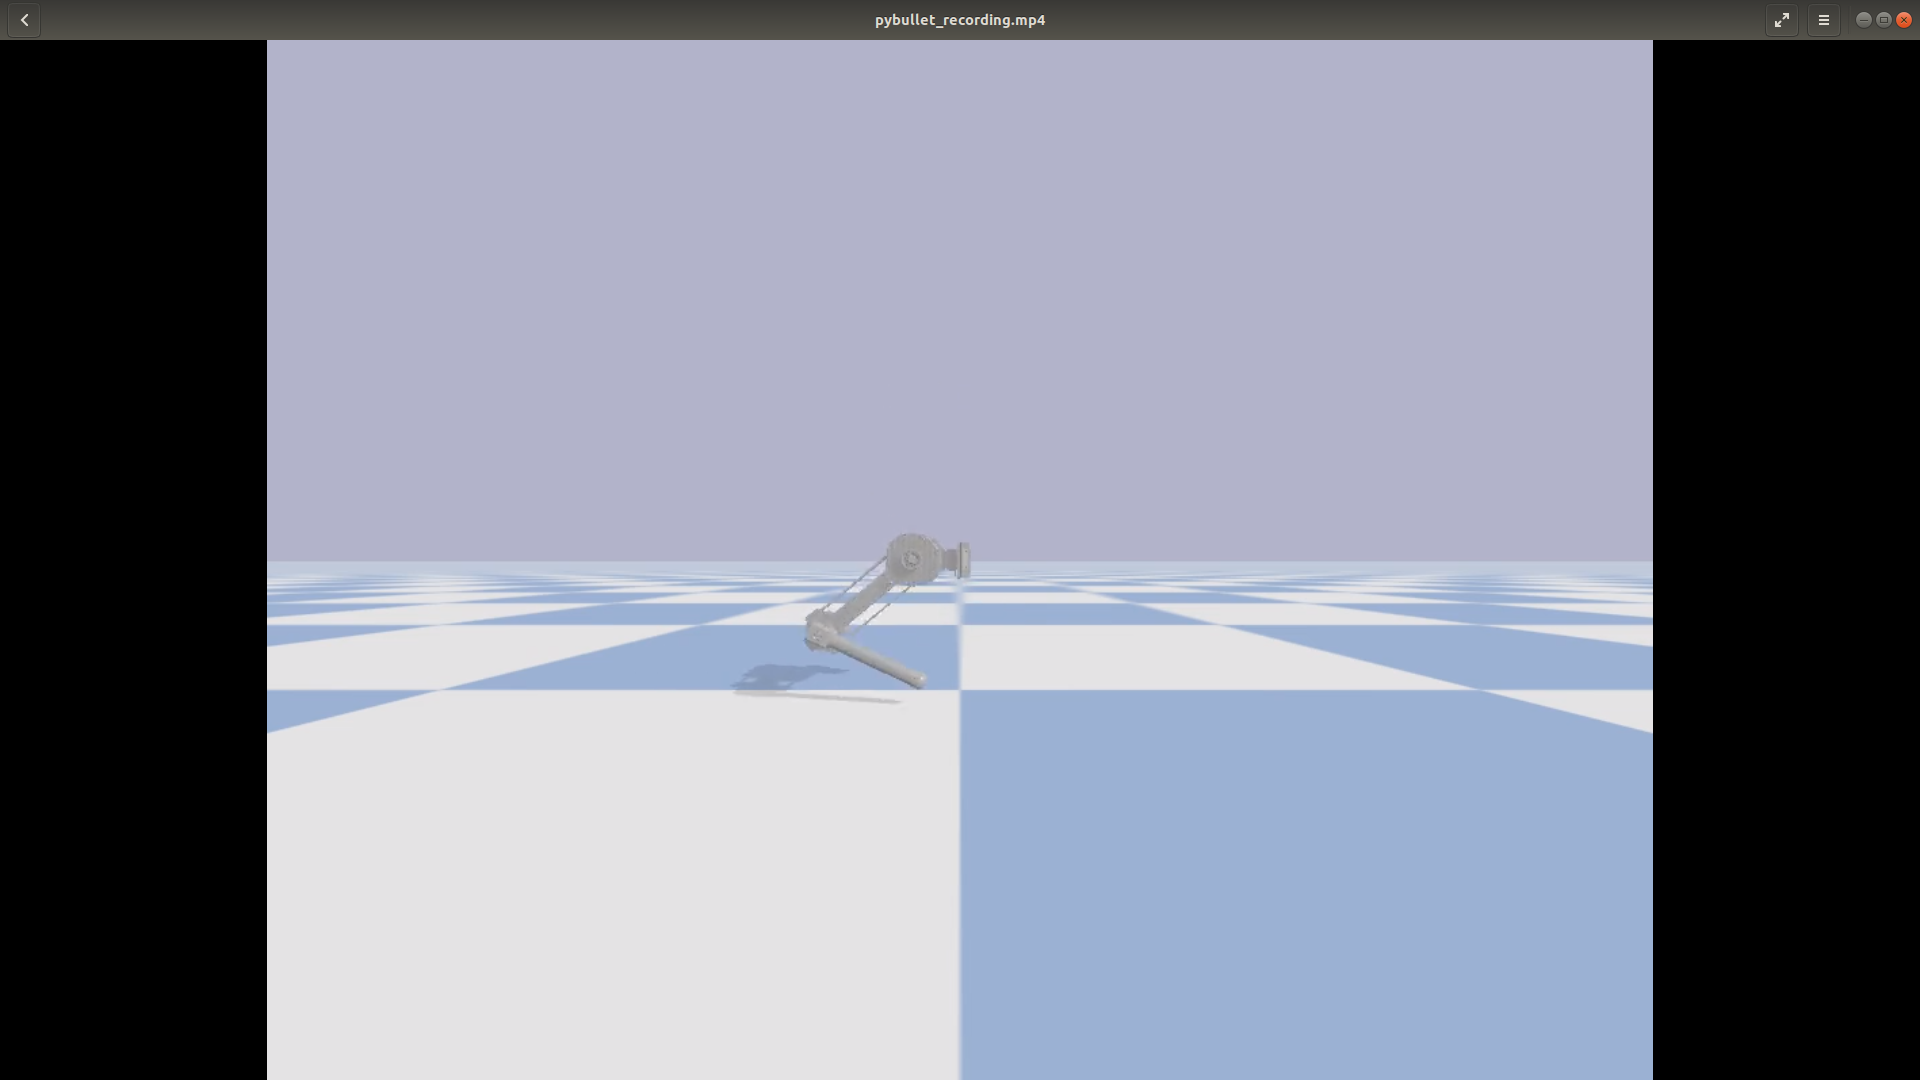
\includegraphics[width=\textwidth, trim={25cm 10cm 25cm 5cm}, clip]{figures/sim0.5m/s54.png}
    \end{subfigure}
    \caption{Simulated jumping sequence for 0.5 m desired height}
    \label{fig:simsequence5}
\end{figure}
\begin{figure}[htb!]
    \centering
    \begin{subfigure}{.24\textwidth}
    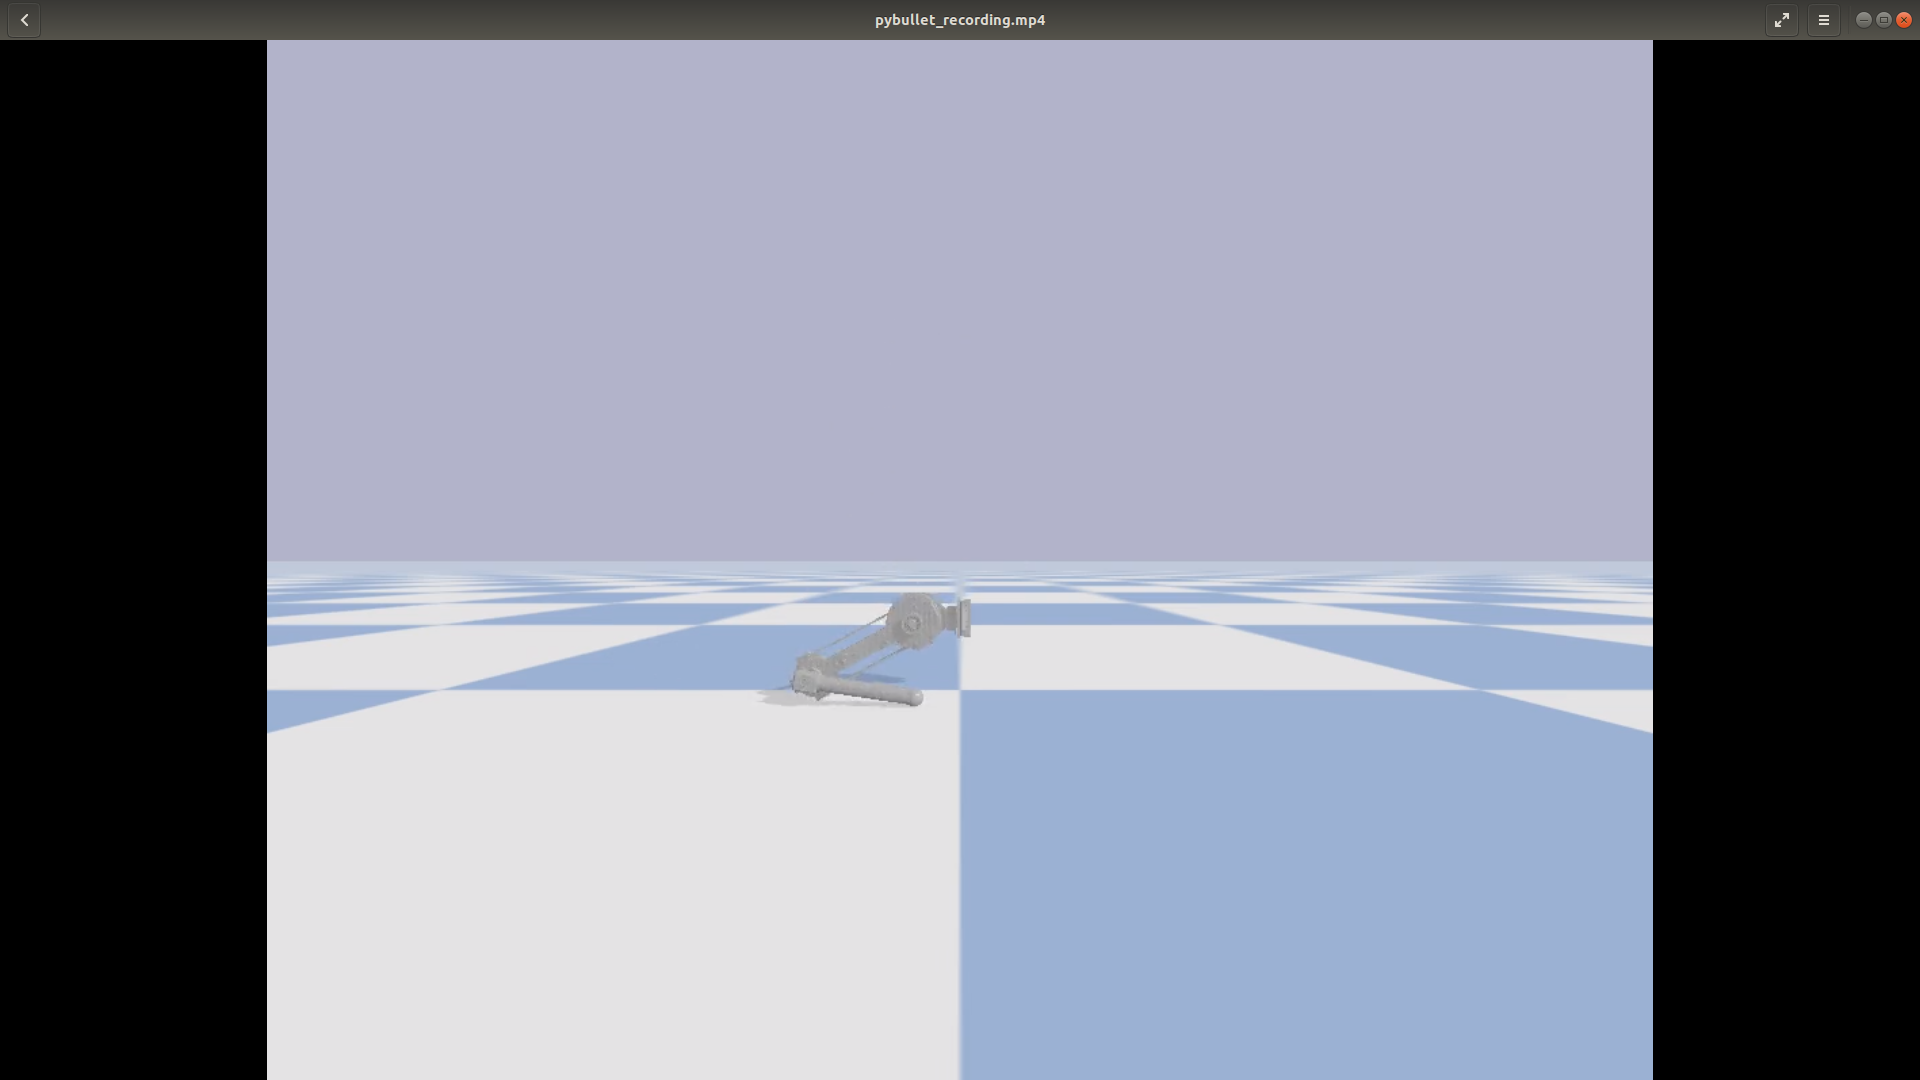
\includegraphics[width=\textwidth, trim={25cm 10cm 25cm 5cm}, clip]{figures/sim0.6m/s61.png}
    \end{subfigure}
    \begin{subfigure}{.24\textwidth}
    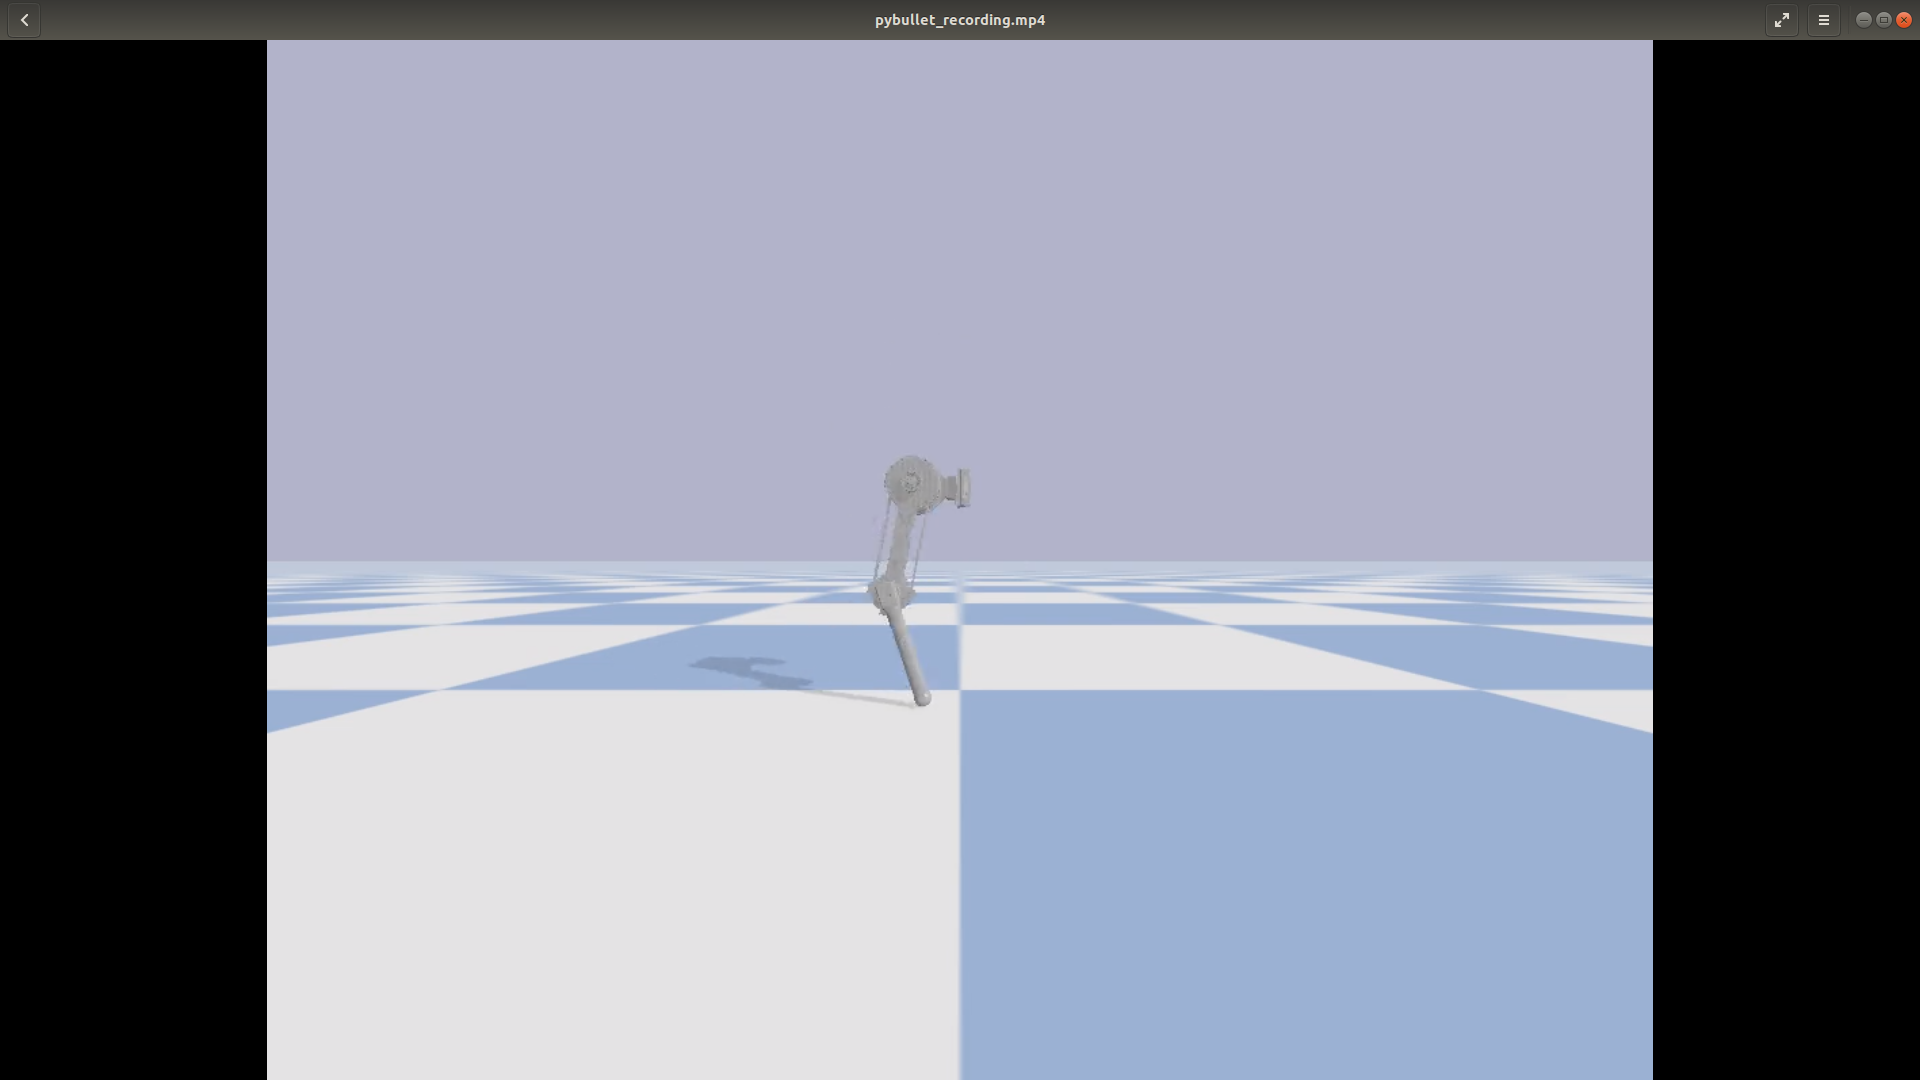
\includegraphics[width=\textwidth, trim={25cm 10cm 25cm 5cm}, clip]{figures/sim0.6m/s62.png}
    \end{subfigure}
    \begin{subfigure}{.24\textwidth}
    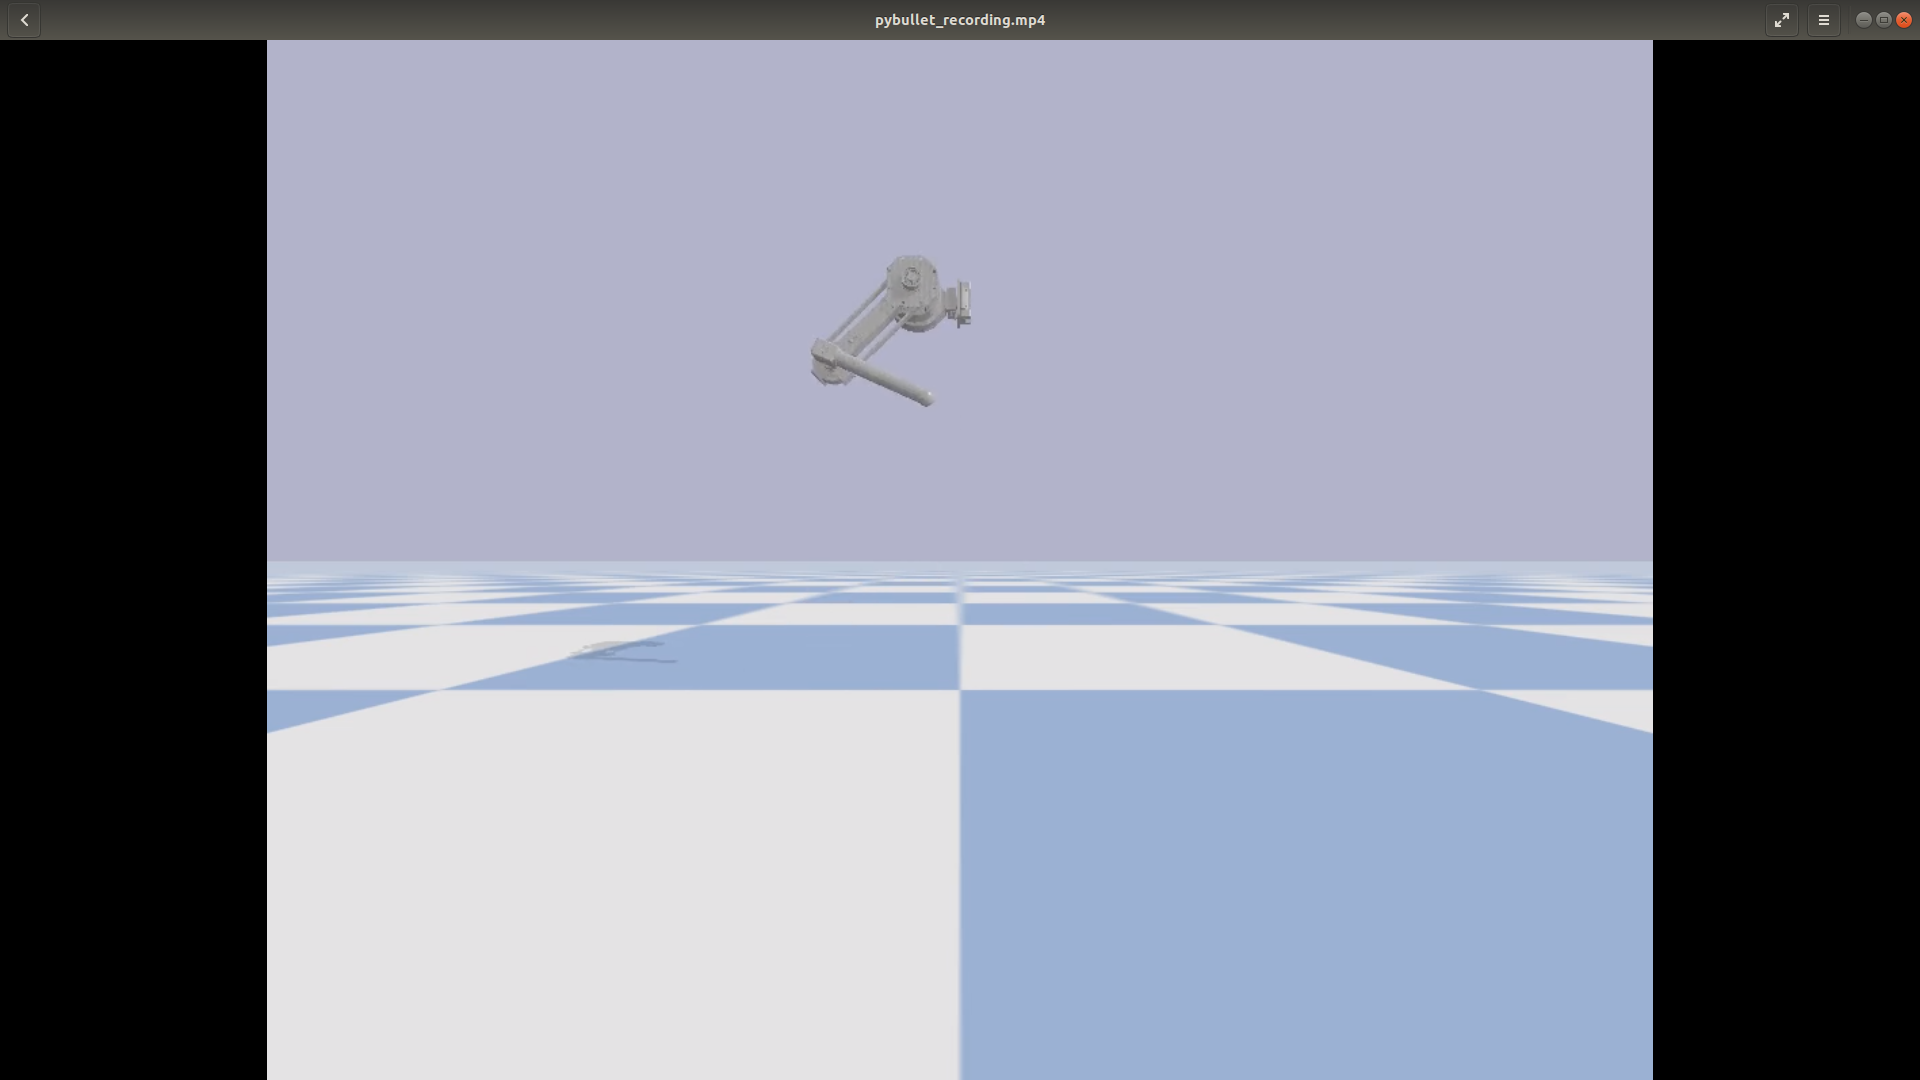
\includegraphics[width=\textwidth, trim={25cm 10cm 25cm 5cm}, clip]{figures/sim0.6m/s63.png}
    \end{subfigure}
    \begin{subfigure}{.24\textwidth}
    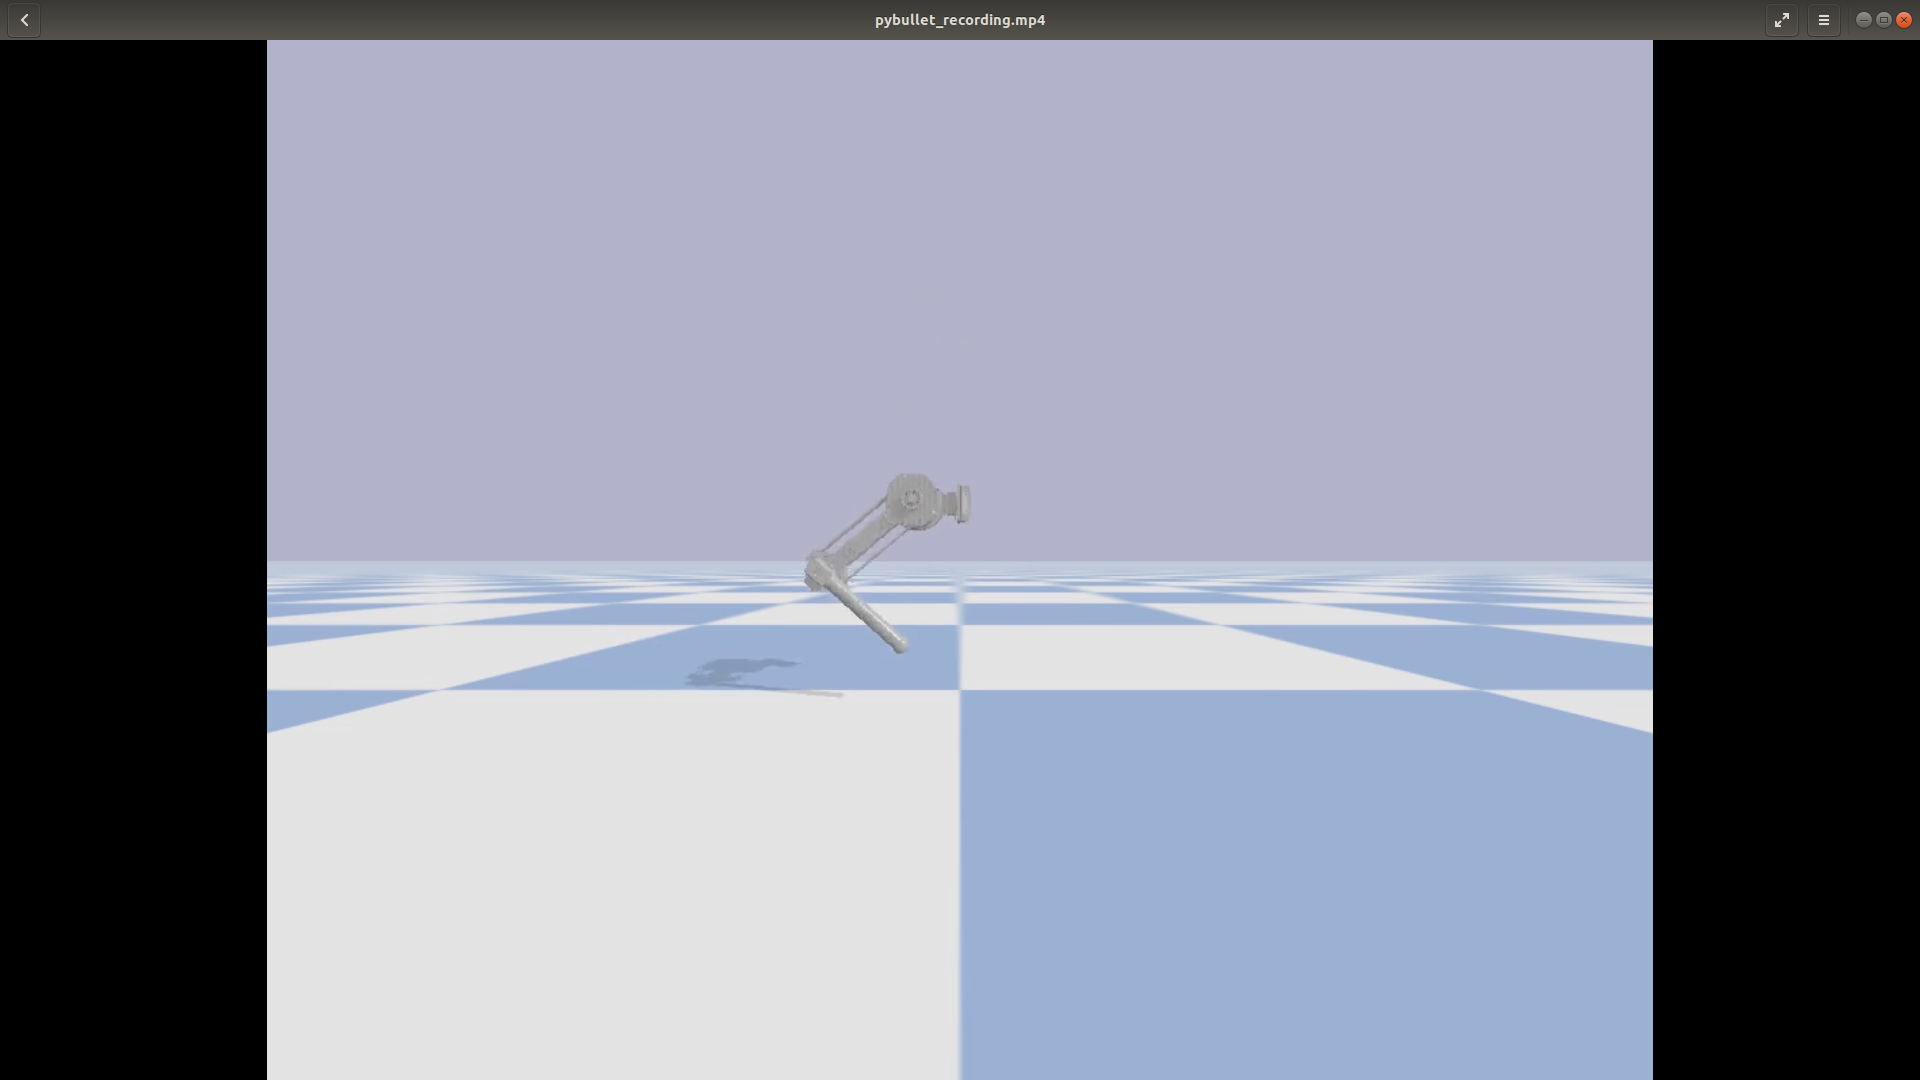
\includegraphics[width=\textwidth, trim={25cm 10cm 25cm 5cm}, clip]{figures/sim0.6m/s64.png}
    \end{subfigure}
    \caption{Simulated jumping sequence for 0.6 m desired height}
    \label{fig:simsequence6}
\end{figure}
% \newpage
If we look at the joint torques (\autoref{fig:simtorque}), we see, that for all three desired heights, we haven't reached the torque limits during the lift-off phase (dark green background). Hence, there is still more potential for higher jumps, even without applying feed forward forces in y-direction as proposed in \autoref{sec:increasingheight}.

% \begin{figure}[htb!]
%     \centering
%     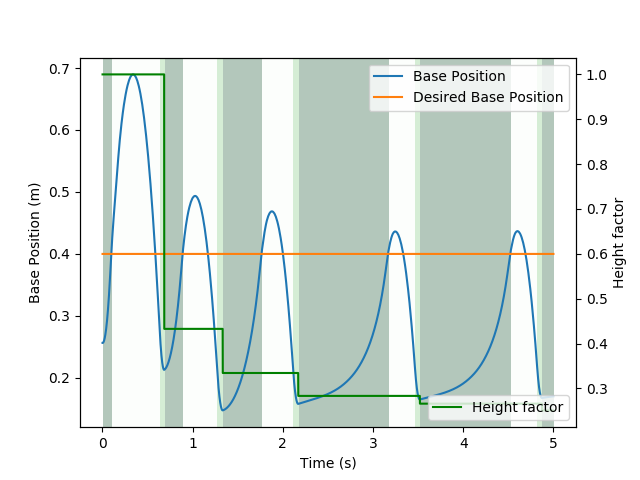
\includegraphics[width=.6\textwidth]{figures/sim0.4m/base_position.png}
%     \caption{Jumping heights with energy shaping control and a desired height of 0.4 m (yellow line) in simulation. The background colour indicates the current phase of the state machine. The flight phase is white, the touchdown phase is light green and the lift-off phase has a dark green background colour.}
%     \label{fig:sim4height}
% \end{figure}
% \begin{figure}[htb!]
%     \centering
%     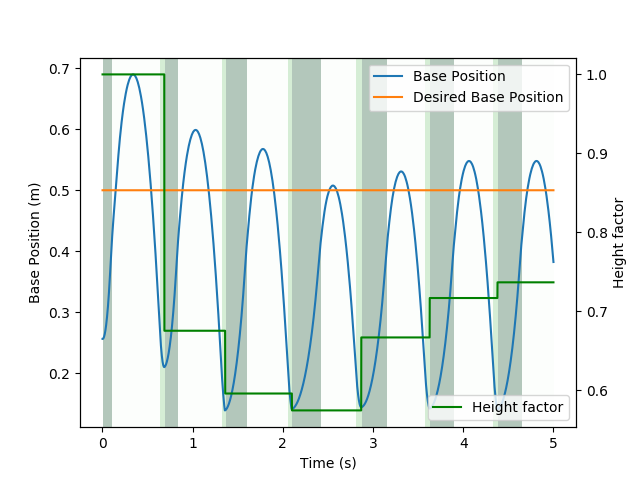
\includegraphics[width=.6\textwidth]{figures/sim0.5m/base_position.png}
%     \caption{Jumping heights with energy shaping control and a desired height of 0.5 m (yellow line) in simulation. The background colour indicates the current phase of the state machine. The flight phase is white, the touchdown phase is light green and the lift-off phase has a dark green background colour.}
%     \label{fig:sim5height}
% \end{figure}
% \begin{figure}[htb!]
%     \centering
%     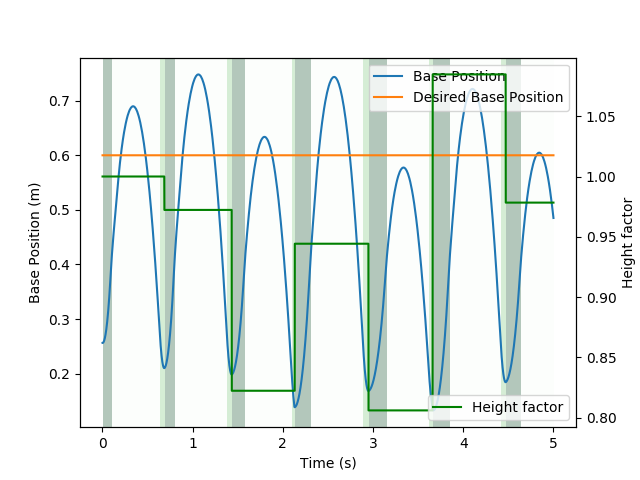
\includegraphics[width=.6\textwidth]{figures/sim0.6m/base_position.png}
%     \caption{Jumping heights with energy shaping control and a desired height of 0.6 m (yellow line) in simulation. The background colour indicates the current phase of the state machine. The flight phase is white, the touchdown phase is light green and the lift-off phase has a dark green background colour.}
%     \label{fig:sim6height}
% \end{figure}

\begin{figure}[htb!]
    \centering
    \begin{subfigure}{.49\textwidth}
    \centering
    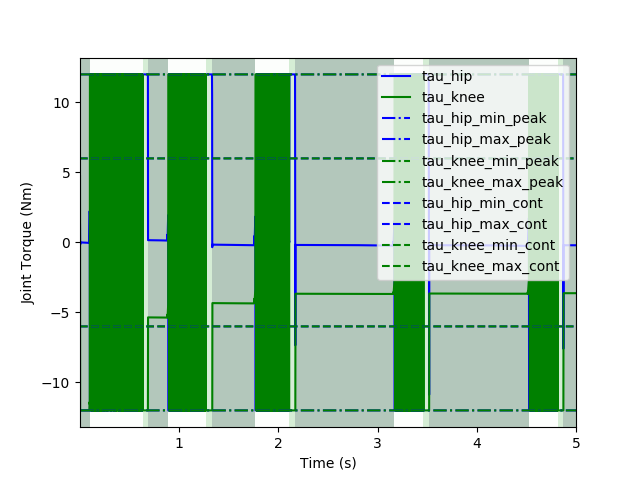
\includegraphics[width=\textwidth]{figures/sim0.4m/joint_efforts.png}
    \subcaption{Desired jumping height: 0.4 m}
    \end{subfigure}
    \begin{subfigure}{.49\textwidth}
    \centering
    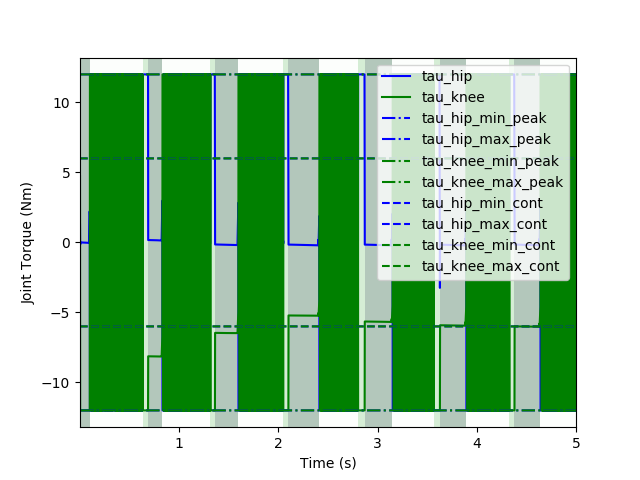
\includegraphics[width=\textwidth]{figures/sim0.5m/joint_efforts.png}
    \subcaption{Desired jumping height: 0.5 m}
    \end{subfigure}
    \begin{subfigure}{.49\textwidth}
    \centering
    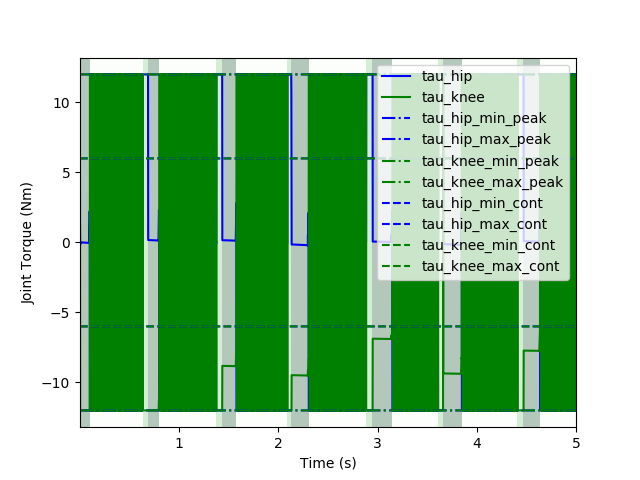
\includegraphics[width=\textwidth]{figures/sim0.6m/joint_efforts.png}
    \subcaption{Desired jumping height: 0.6 m}
    \end{subfigure}
    \caption{Torque of the energy shaping control simulation with a desired height of 0.4 m (a), 0.5 m (b) and 0.6 m (c). The background colour indicates the current phase of the state machine. The flight phase is white, the touchdown phase is light green and the lift-off phase has a dark green background colour.}
    \label{fig:simtorque}
\end{figure}








% \begin{figure}[htb!]
%     \centering
%     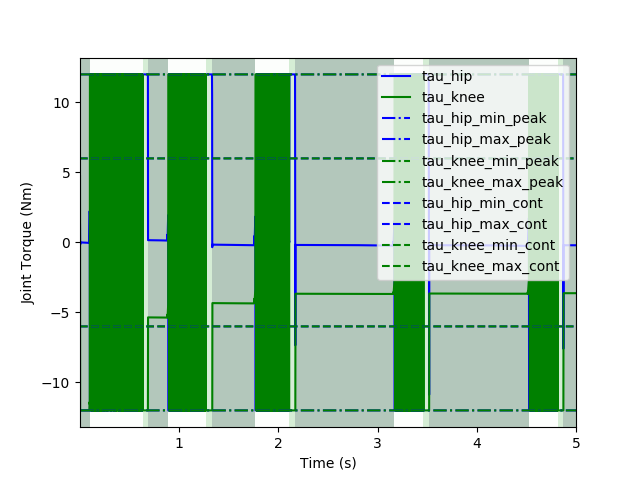
\includegraphics[width=.6\textwidth]{figures/sim0.4m/joint_efforts.png}
%     \caption{Torque of the energy shaping control simulation with a desired height of 0.4 m. The background colour indicates the current phase of the state machine. The flight phase is white, the touchdown phase is light green and the lift-off phase has a dark green background colour. }
%     \label{fig:sim4torque}
% \end{figure}
% \begin{figure}[htb!]
%     \centering
%     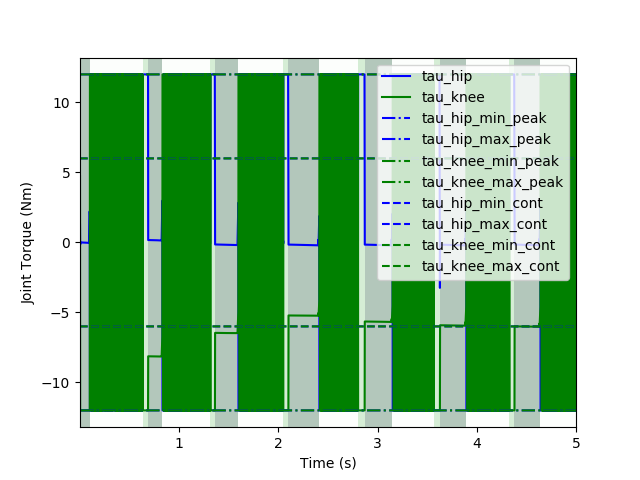
\includegraphics[width=.6\textwidth]{figures/sim0.5m/joint_efforts.png}
%     \caption{Torque of the energy shaping control simulation with a desired height of 0.5 m. The background colour indicates the current phase of the state machine. The flight phase is white, the touchdown phase is light green and the lift-off phase has a dark green background colour.}
%     \label{fig:5simtorque}
% \end{figure}
% \begin{figure}[htb!]
%     \centering
%     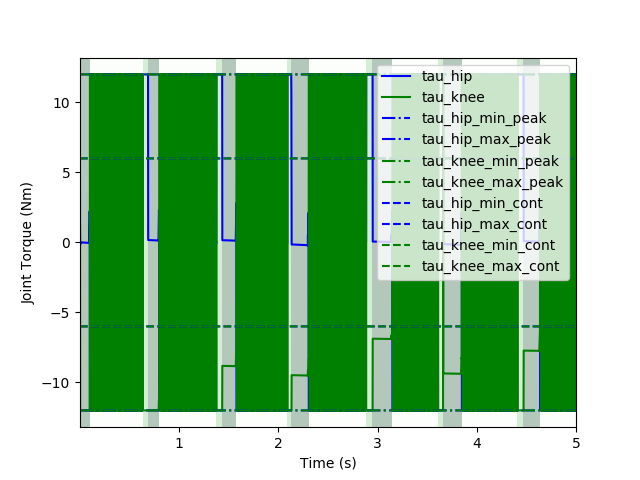
\includegraphics[width=.6\textwidth]{figures/sim0.6m/joint_efforts.png}
%     \caption{Torque of the energy shaping control simulation with a desired height of 0.6 m. The background colour indicates the current phase of the state machine. The flight phase is white, the touchdown phase is light green and the lift-off phase has a dark green background colour.}
%     \label{fig:sim6torque}
% \end{figure}


% Implementing a state machine for the simulation is comparably easy, since contract recognition works reliable and thus, the simulation recognize all states  without long fine-tuning.  Hence, the main tuning parameters are the gains and desired joint positions.
% Here we see, that it is quite difficult to prevent the hopping leg from sliding on the ground and stabilizing its trajectory during flight. 


\clearpage
\section{Hopping control in the real system}
In the real system we observed, that the  energy shaping control was able to reach preset jumping heights of 0.4 m (see \autoref{fig:4height}), 0.5 m (see \autoref{fig:5height}) and 0.6 m (see \autoref{fig:6height}) according to the estimated state. By observing the torques during these jumps (\autoref{fig:4torque}, \ref{fig:5torque} and \ref{fig:6torque}) we can see, that during the lift-off phase (dark green background) the applied torques increase for higher jumping heights. At 0.6 meters, the straight part of the desired elbow torques indicates, that the torques are clipped due to the motor torque limits. Hence, the elbow cannot apply higher torques, and we reached the limit of the energy shaping controller in combination with the commanded feed forward force of 15 N in y-direction (see \autoref{sec:increasingheight}). 

If we compare the state estimation with the video sequences, we took during the jumping trials (see \autoref{fig:sequence4}, \ref{fig:sequence5} and \ref{fig:sequence6}) we can see, that the jumping height was a bit overestimated, especially for the desired height of 0.6 m we actually just reached about 0.58 m (see \autoref{fig:sequence6}).
\begin{figure}[htb!]
    \centering
    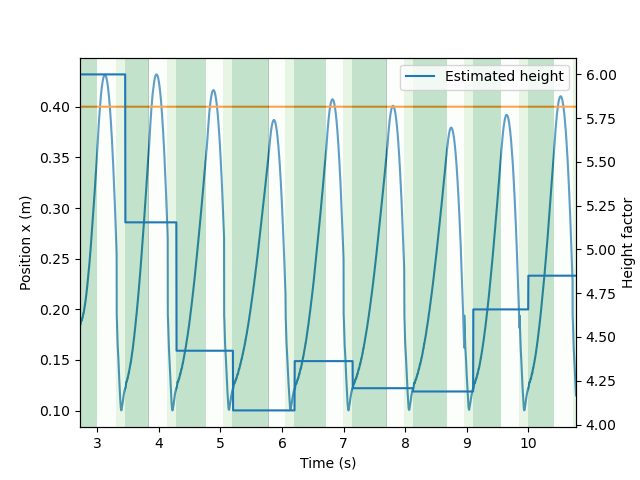
\includegraphics[width=.6\textwidth]{figures/0.4m/height.png}
    \caption{Jumping heights with energy shaping control and a desired height of 0.4 m (yellow line). The height of the base is printed with the sin like blue line, and the height factor $k_i$ is printed with the stabbed blue line on the secondary y-axis. The background colour indicates the current phase of the state machine. The flight phase is white, the touchdown phase is light green and the lift-off phase has a dark green background colour.}
    \label{fig:4height}
\end{figure}
\begin{figure}[htb!]
    \centering
    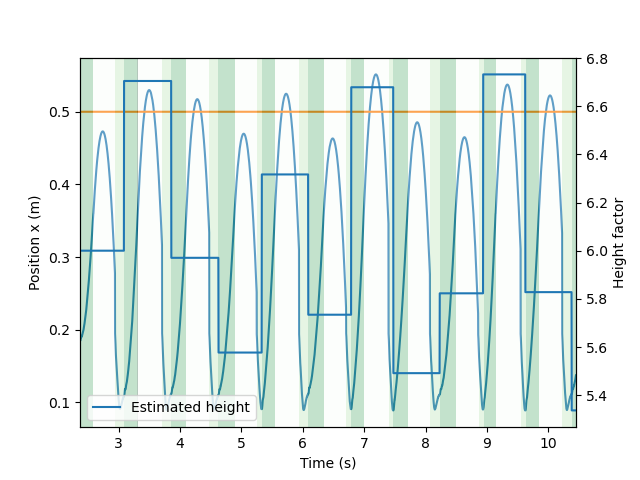
\includegraphics[width=.6\textwidth]{figures/0.5m/height.png}
    \caption{Jumping heights with energy shaping control and a desired height of 0.5 m (yellow line). The height of the base is printed with the sin like blue line, and the height factor $k_i$ is printed with the stabbed blue line on the secondary y-axis. The background colour indicates the current phase of the state machine. The flight phase is white, the touchdown phase is light green and the lift-off phase has a dark green background colour.}
    \label{fig:5height}
\end{figure}
\begin{figure}[htb!]
    \centering
    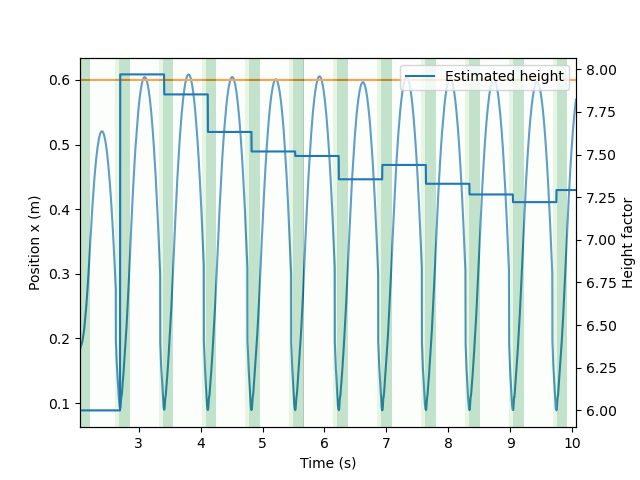
\includegraphics[width=.6\textwidth]{figures/0.6m/height.png}
    \caption{Jumping heights with energy shaping control and a desired height of 0.6 m (yellow line). The height of the base is printed with the sin like blue line, and the height factor $k_i$ is printed with the stabbed blue line on the secondary y-axis. The background colour indicates the current phase of the state machine. The flight phase is white, the touchdown phase is light green and the lift-off phase has a dark green background colour.}
    \label{fig:6height}
\end{figure}


\begin{figure}[htb!]
    \centering
    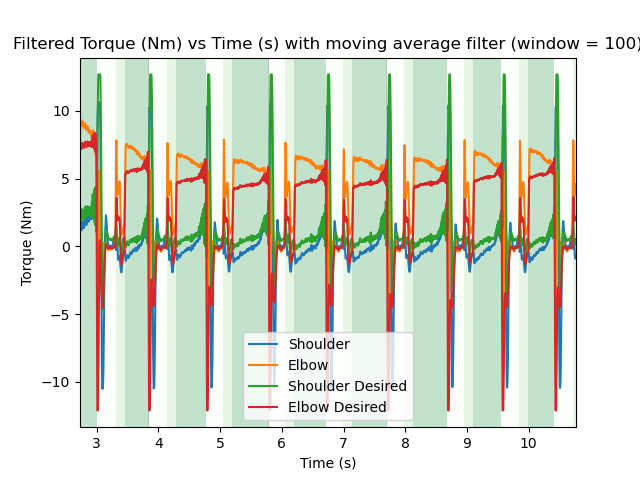
\includegraphics[width=.6\textwidth]{figures/0.4m/filtered_torque.png}
    \caption{Filtered torque of the energy shaping control with a desired height of 0.4 m. The background colour indicates the current phase of the state machine. The flight phase is white, the touchdown phase is light green and the lift-off phase has a dark green background colour. }
    \label{fig:4torque}
\end{figure}
\begin{figure}[htb!]
    \centering
    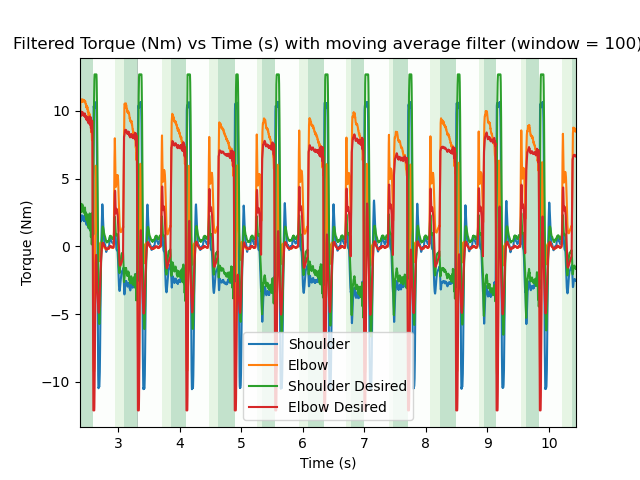
\includegraphics[width=.6\textwidth]{figures/0.5m/filtered_torque.png}
    \caption{Filtered torque of the energy shaping control with a desired height of 0.5 m. The background colour indicates the current phase of the state machine. The flight phase is white, the touchdown phase is light green and the lift-off phase has a dark green background colour.}
    \label{fig:5torque}
\end{figure}
\begin{figure}[htb!]
    \centering
    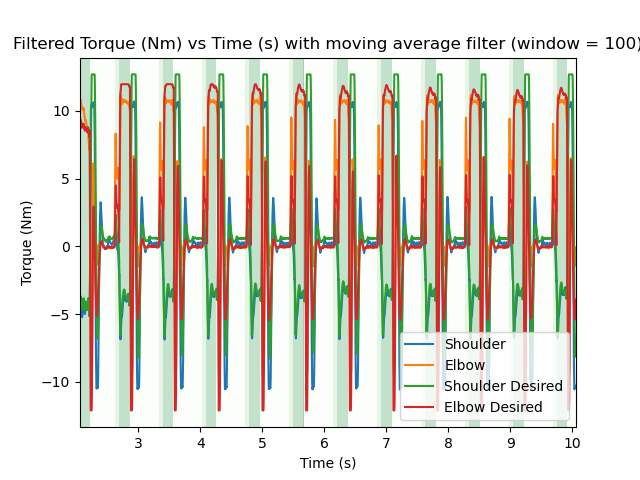
\includegraphics[width=.6\textwidth]{figures/0.6m/filtered_torque.png}
    \caption{Filtered torque of the energy shaping control with a desired height of 0.6 m. The background colour indicates the current phase of the state machine. The flight phase is white, the touchdown phase is light green and the lift-off phase has a dark green background colour.}
    \label{fig:6torque}
\end{figure}


\begin{figure}[htb!]
    \centering
    \begin{subfigure}{.24\textwidth}
    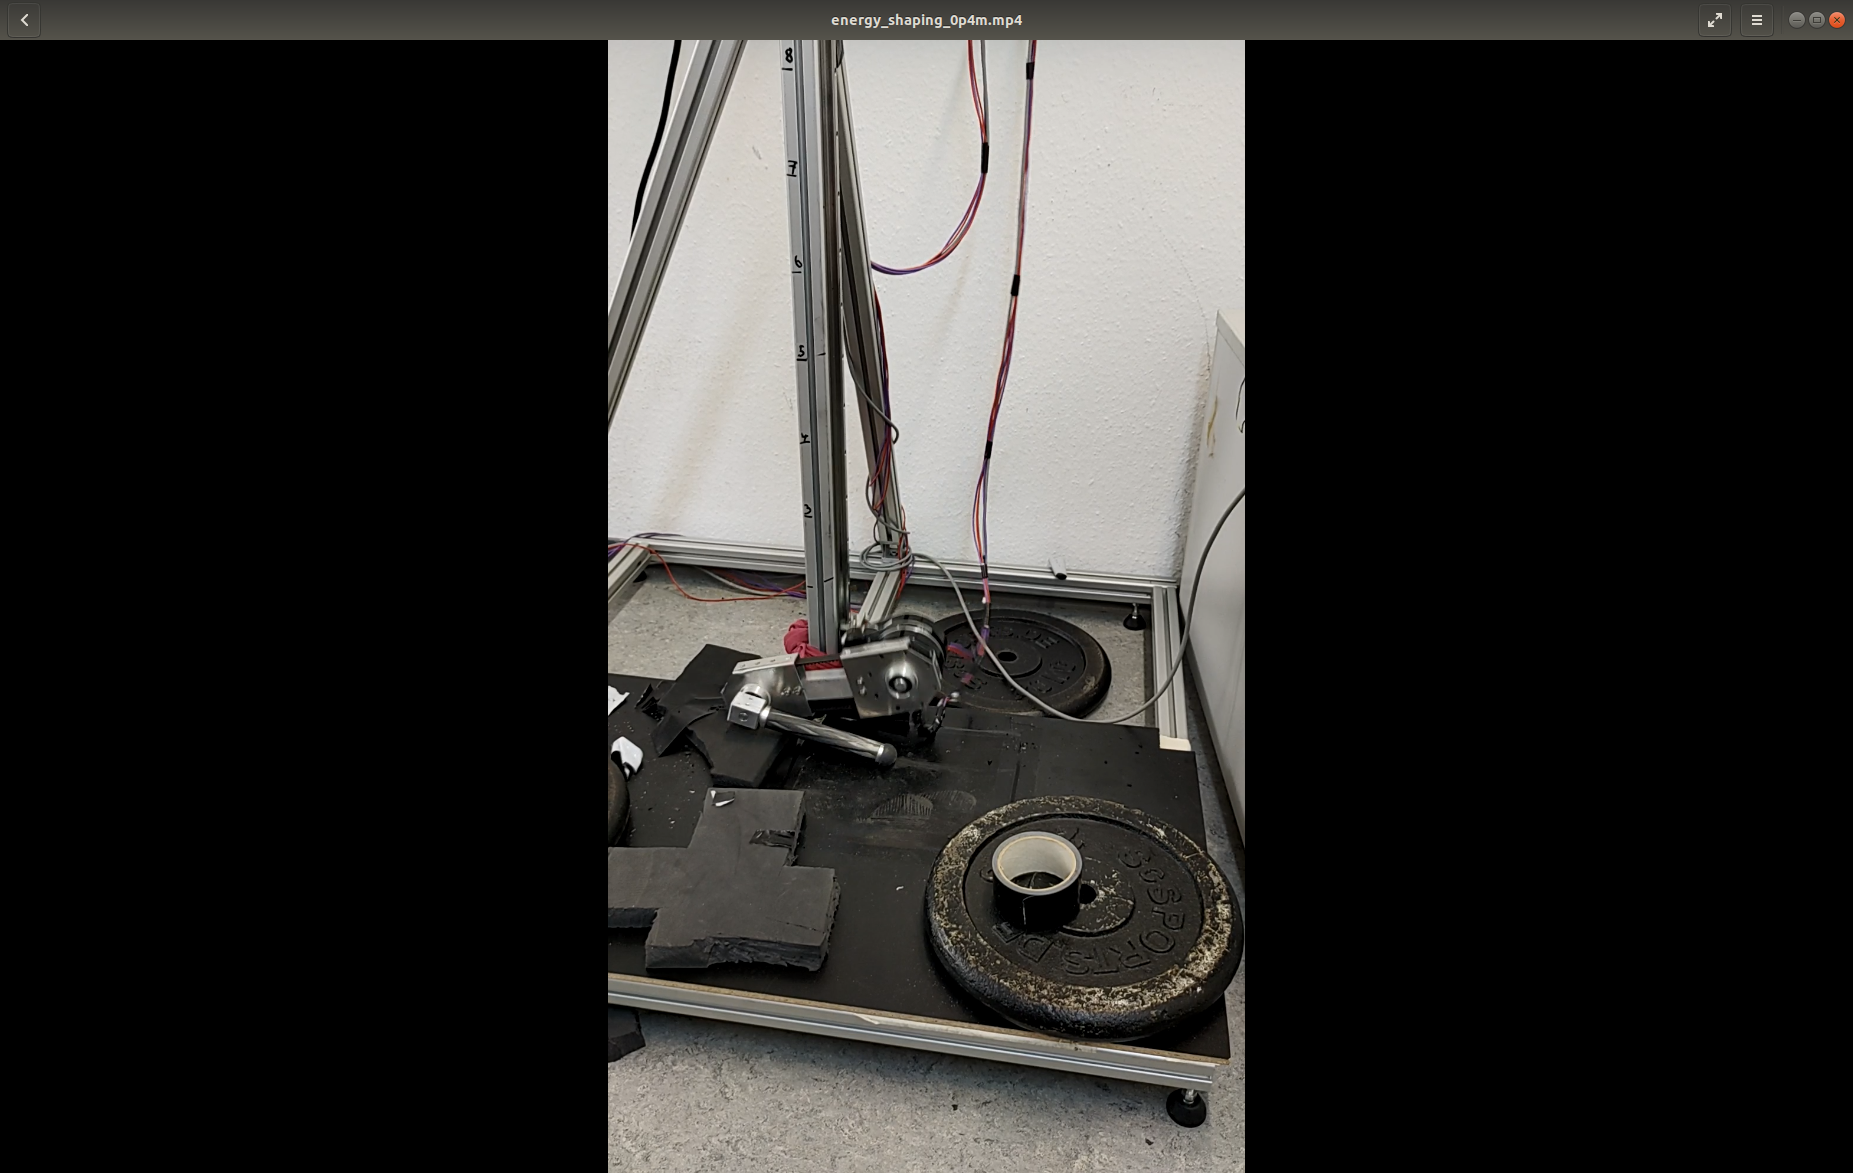
\includegraphics[width=\textwidth, trim={25cm 10cm 25cm 10cm}, clip]{figures/0.4m/p4m1.png}
    \end{subfigure}
    \begin{subfigure}{.24\textwidth}
    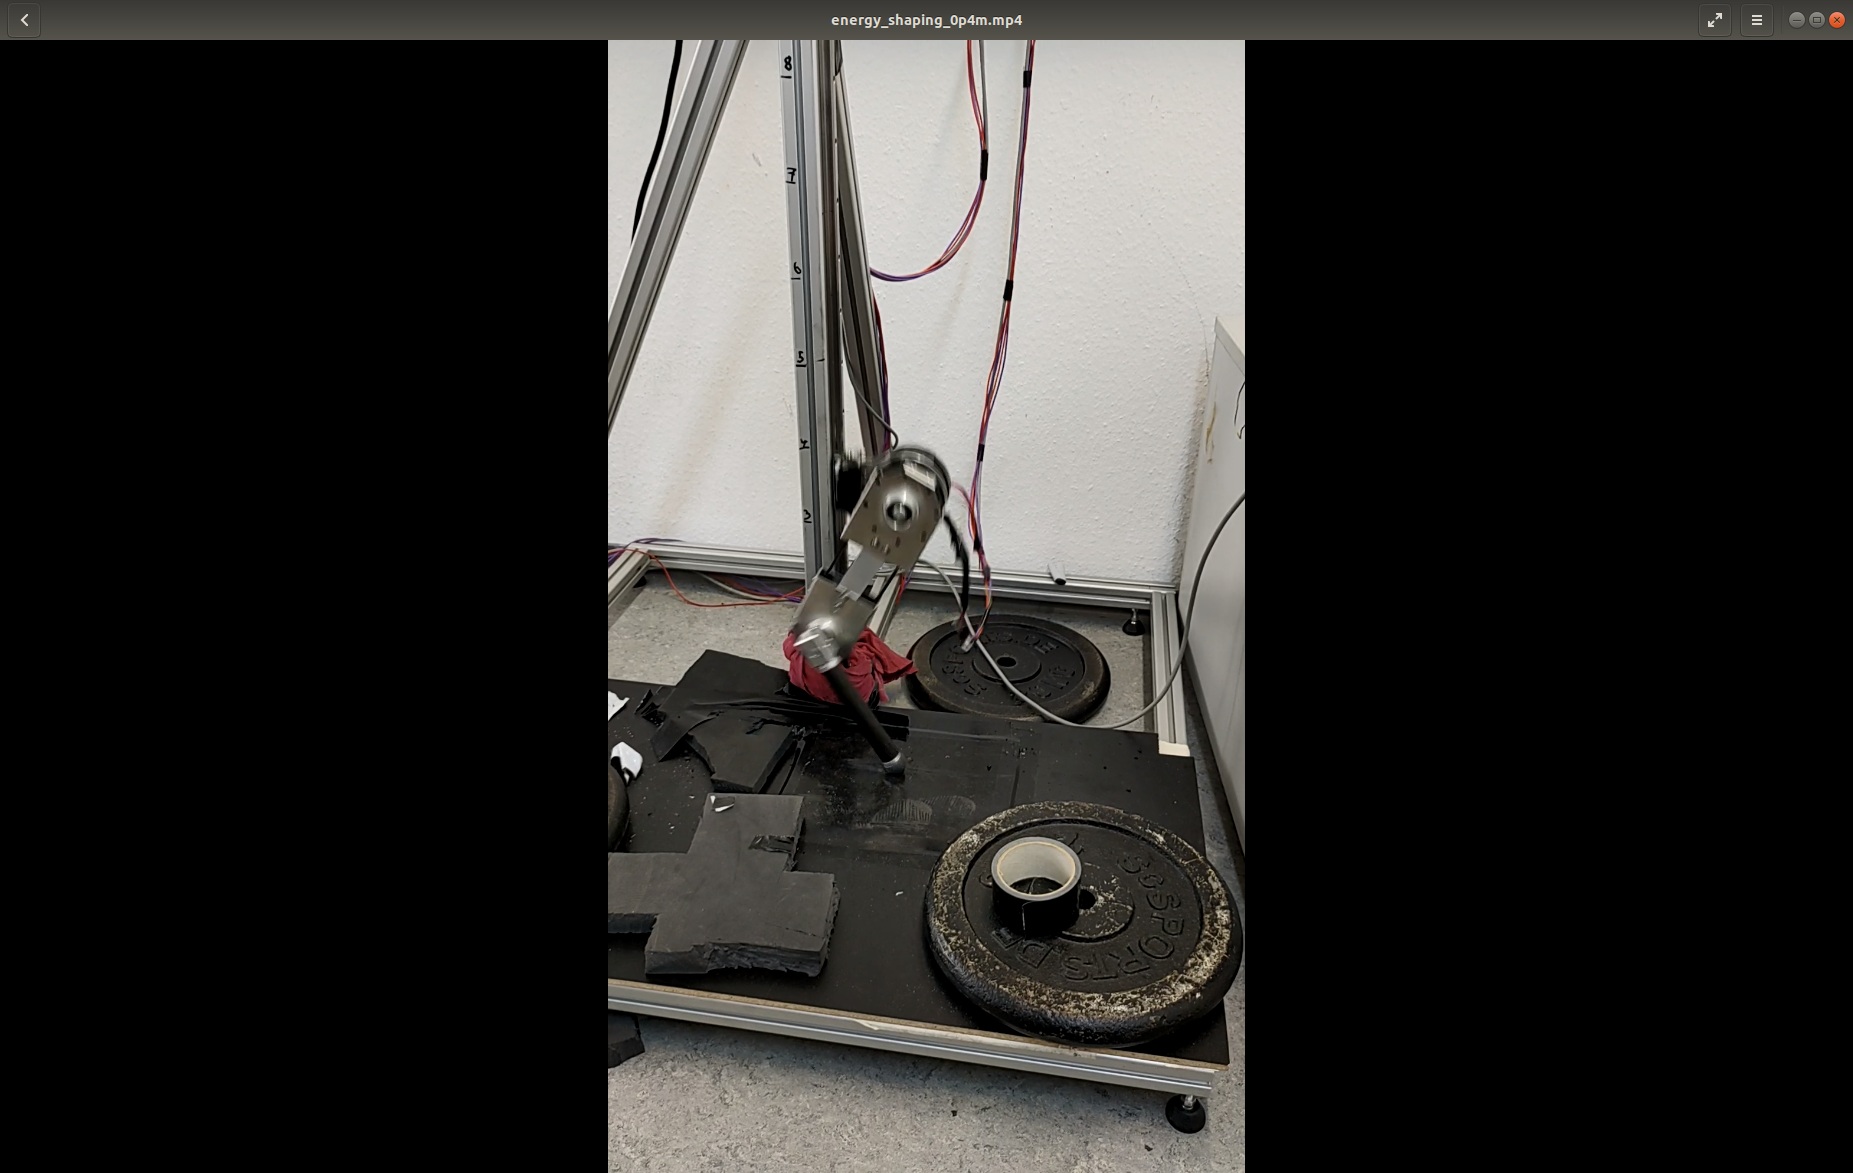
\includegraphics[width=\textwidth, trim={25cm 10cm 25cm 10cm}, clip]{figures/0.4m/p4m2.png}
    \end{subfigure}
    \begin{subfigure}{.24\textwidth}
    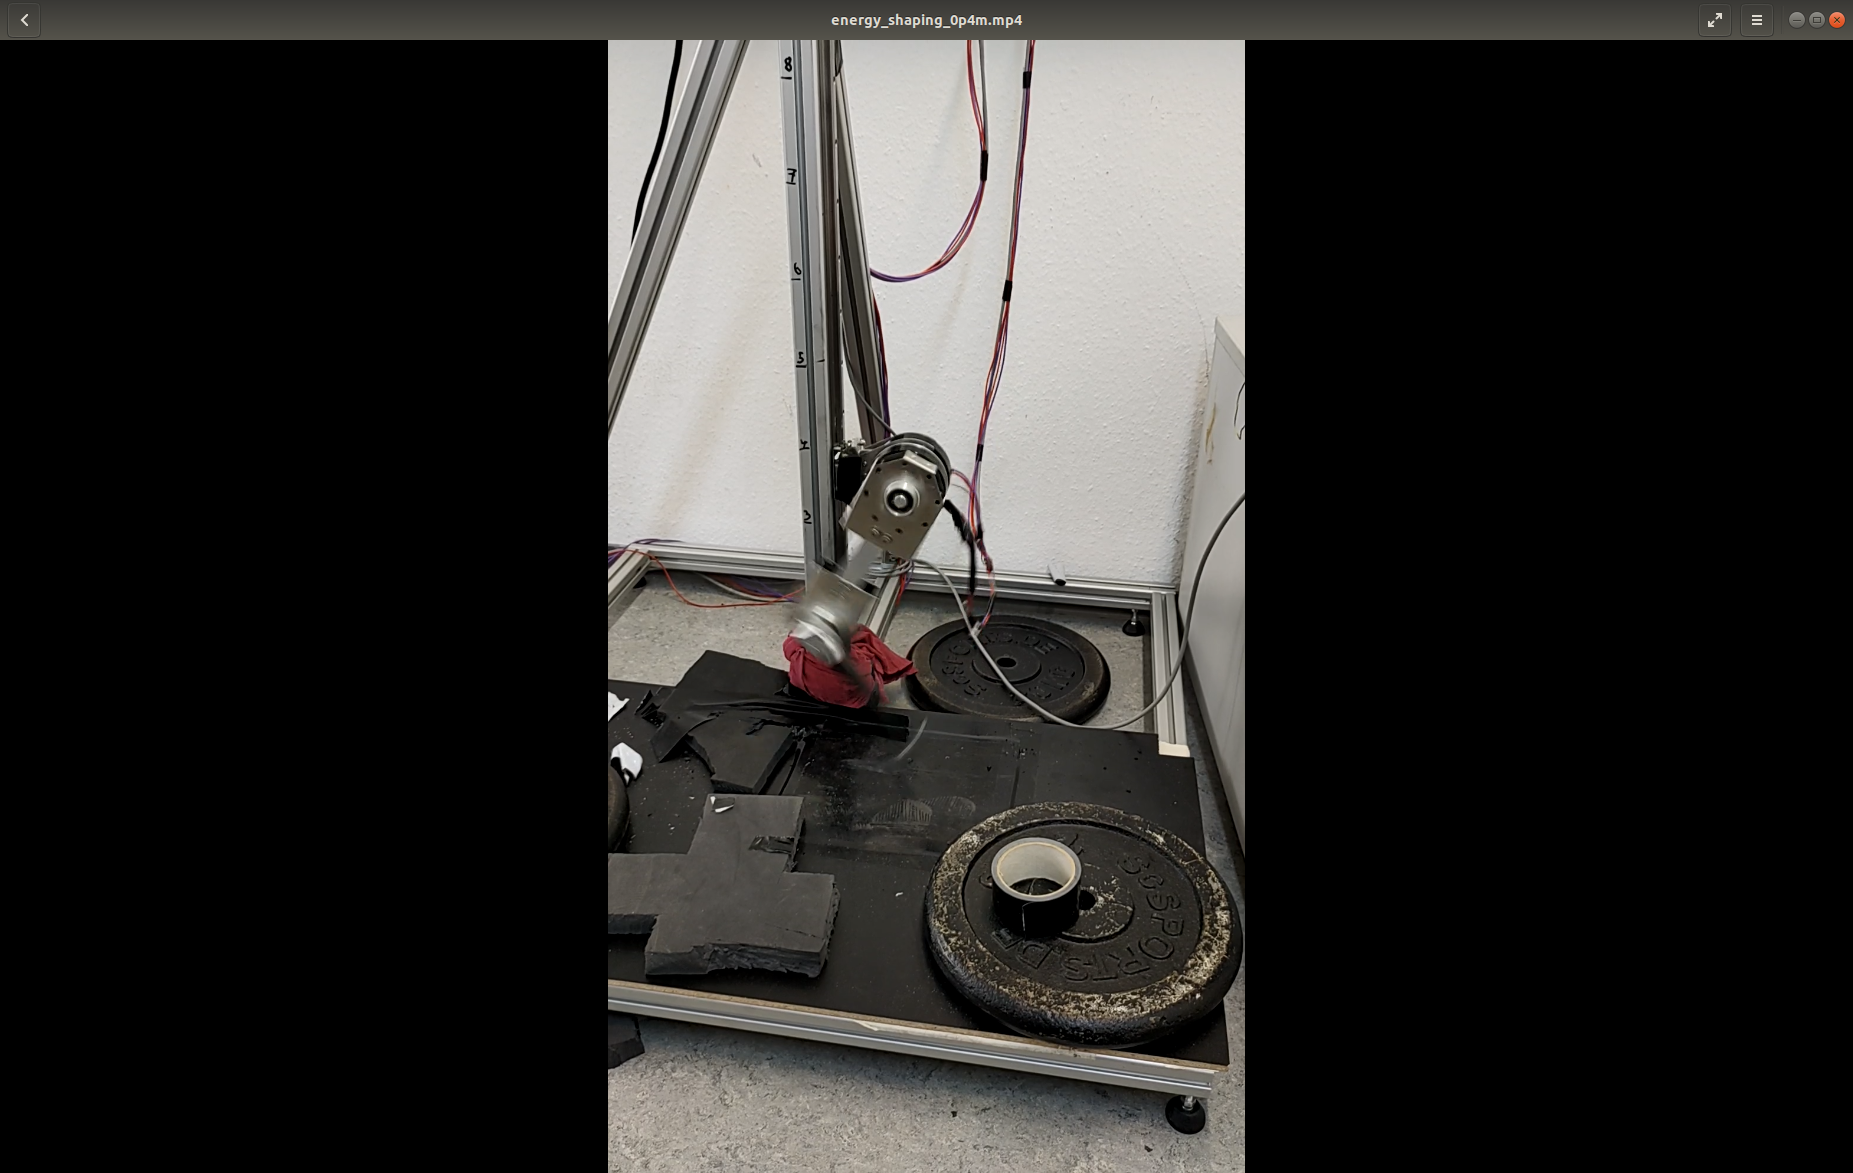
\includegraphics[width=\textwidth, trim={25cm 10cm 25cm 10cm}, clip]{figures/0.4m/p4m3.png}
    \end{subfigure}
    \begin{subfigure}{.24\textwidth}
    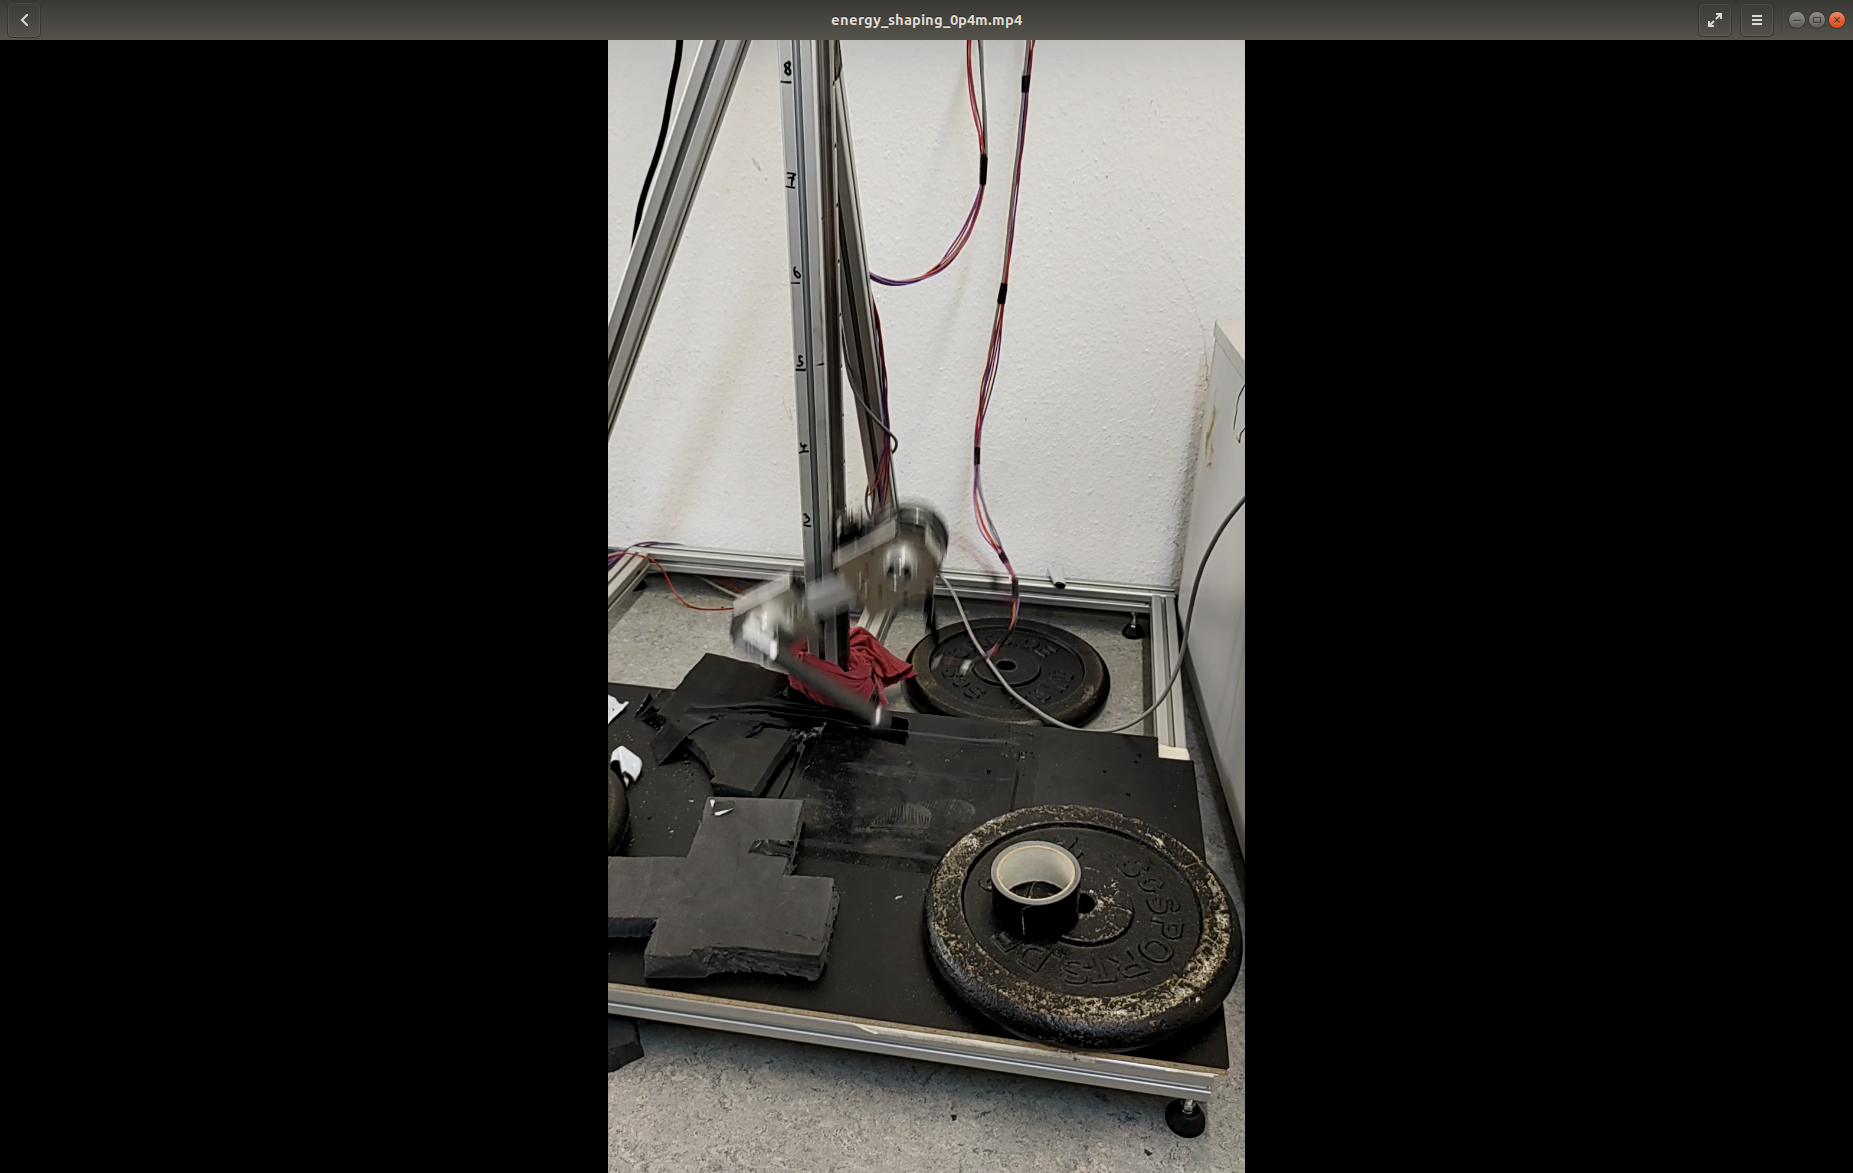
\includegraphics[width=\textwidth, trim={25cm 10cm 25cm 10cm}, clip]{figures/0.4m/p4m4.png}
    \end{subfigure}
    \caption{Jumping sequence for 0.4 m desired height}
    \label{fig:sequence4}
\end{figure}



\begin{figure}[htb!]
    \centering
    \begin{subfigure}{.24\textwidth}
    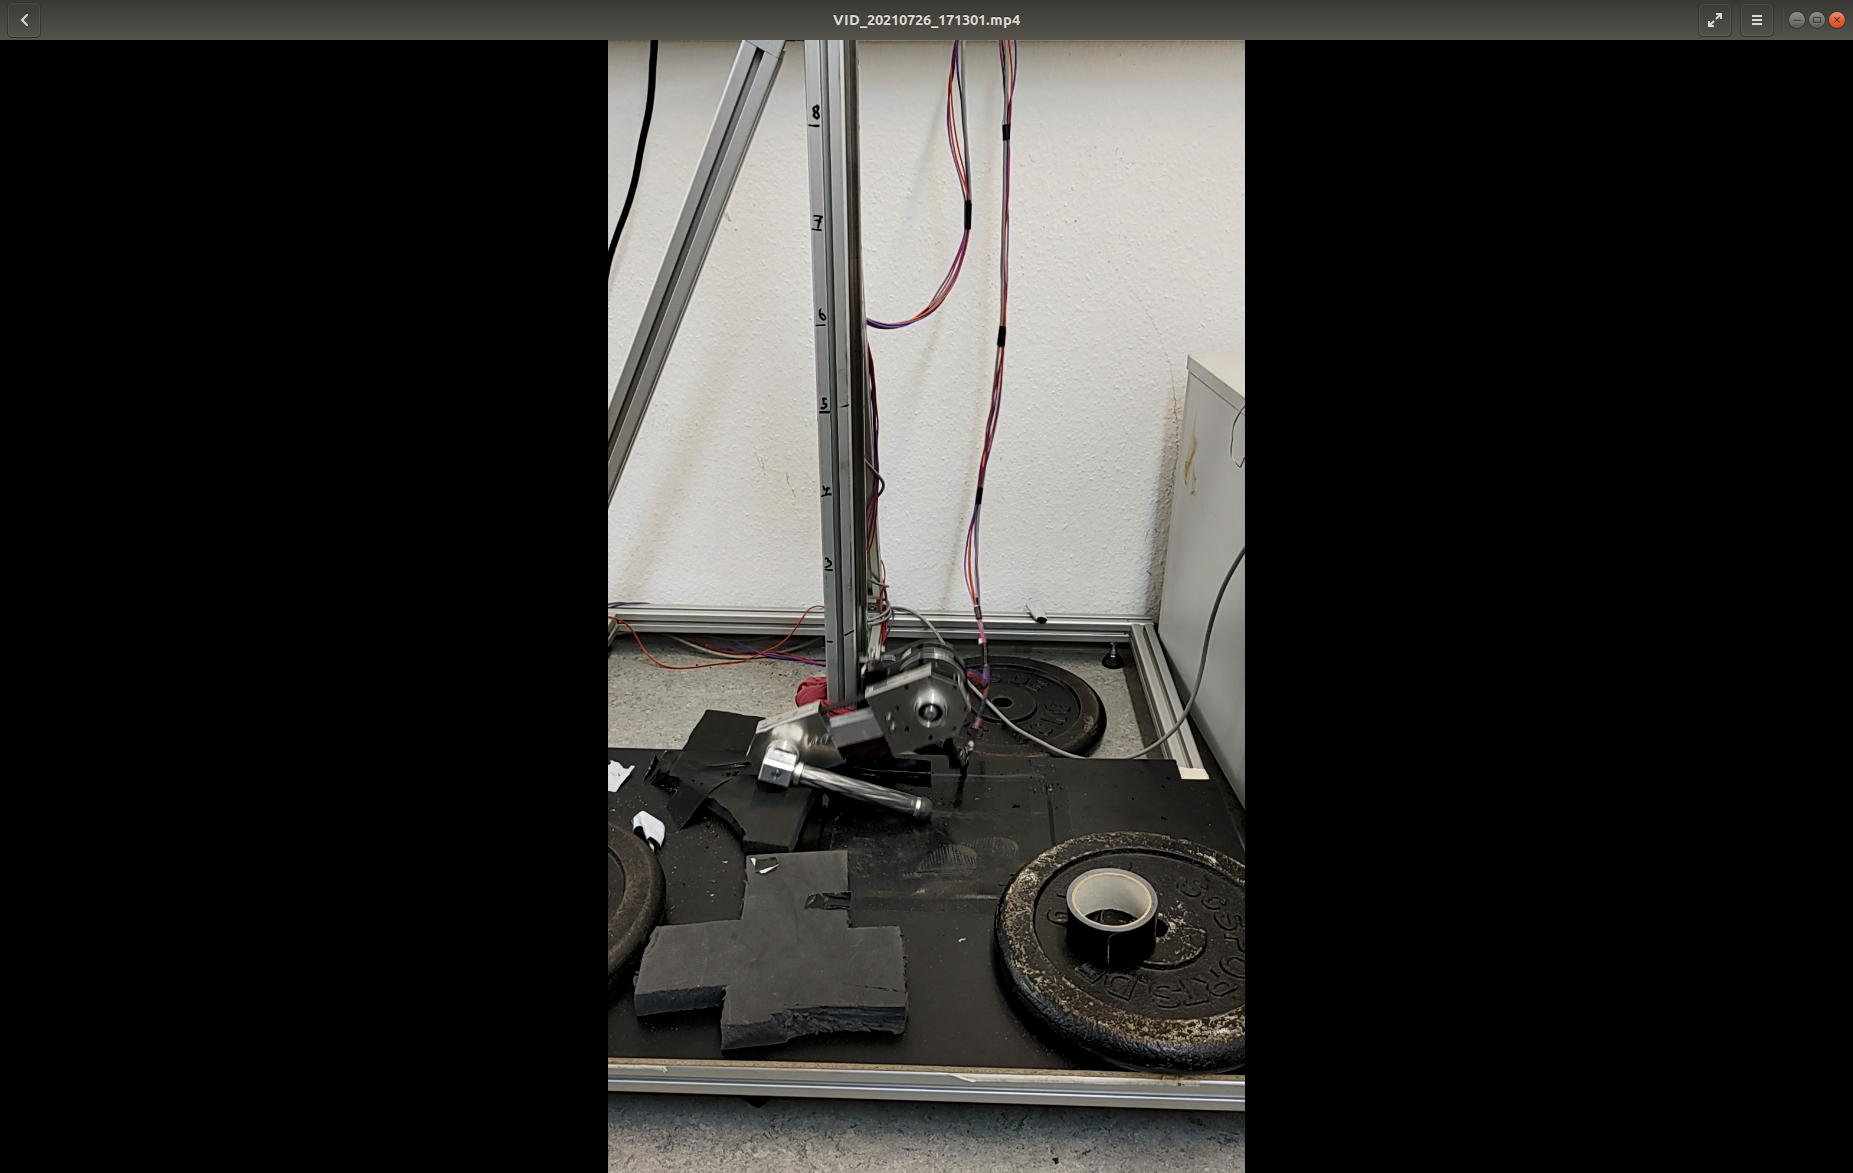
\includegraphics[width=\textwidth, trim={25cm 10cm 25cm 10cm}, clip]{figures/0.5m/p5m1.png}
    \end{subfigure}
    \begin{subfigure}{.24\textwidth}
    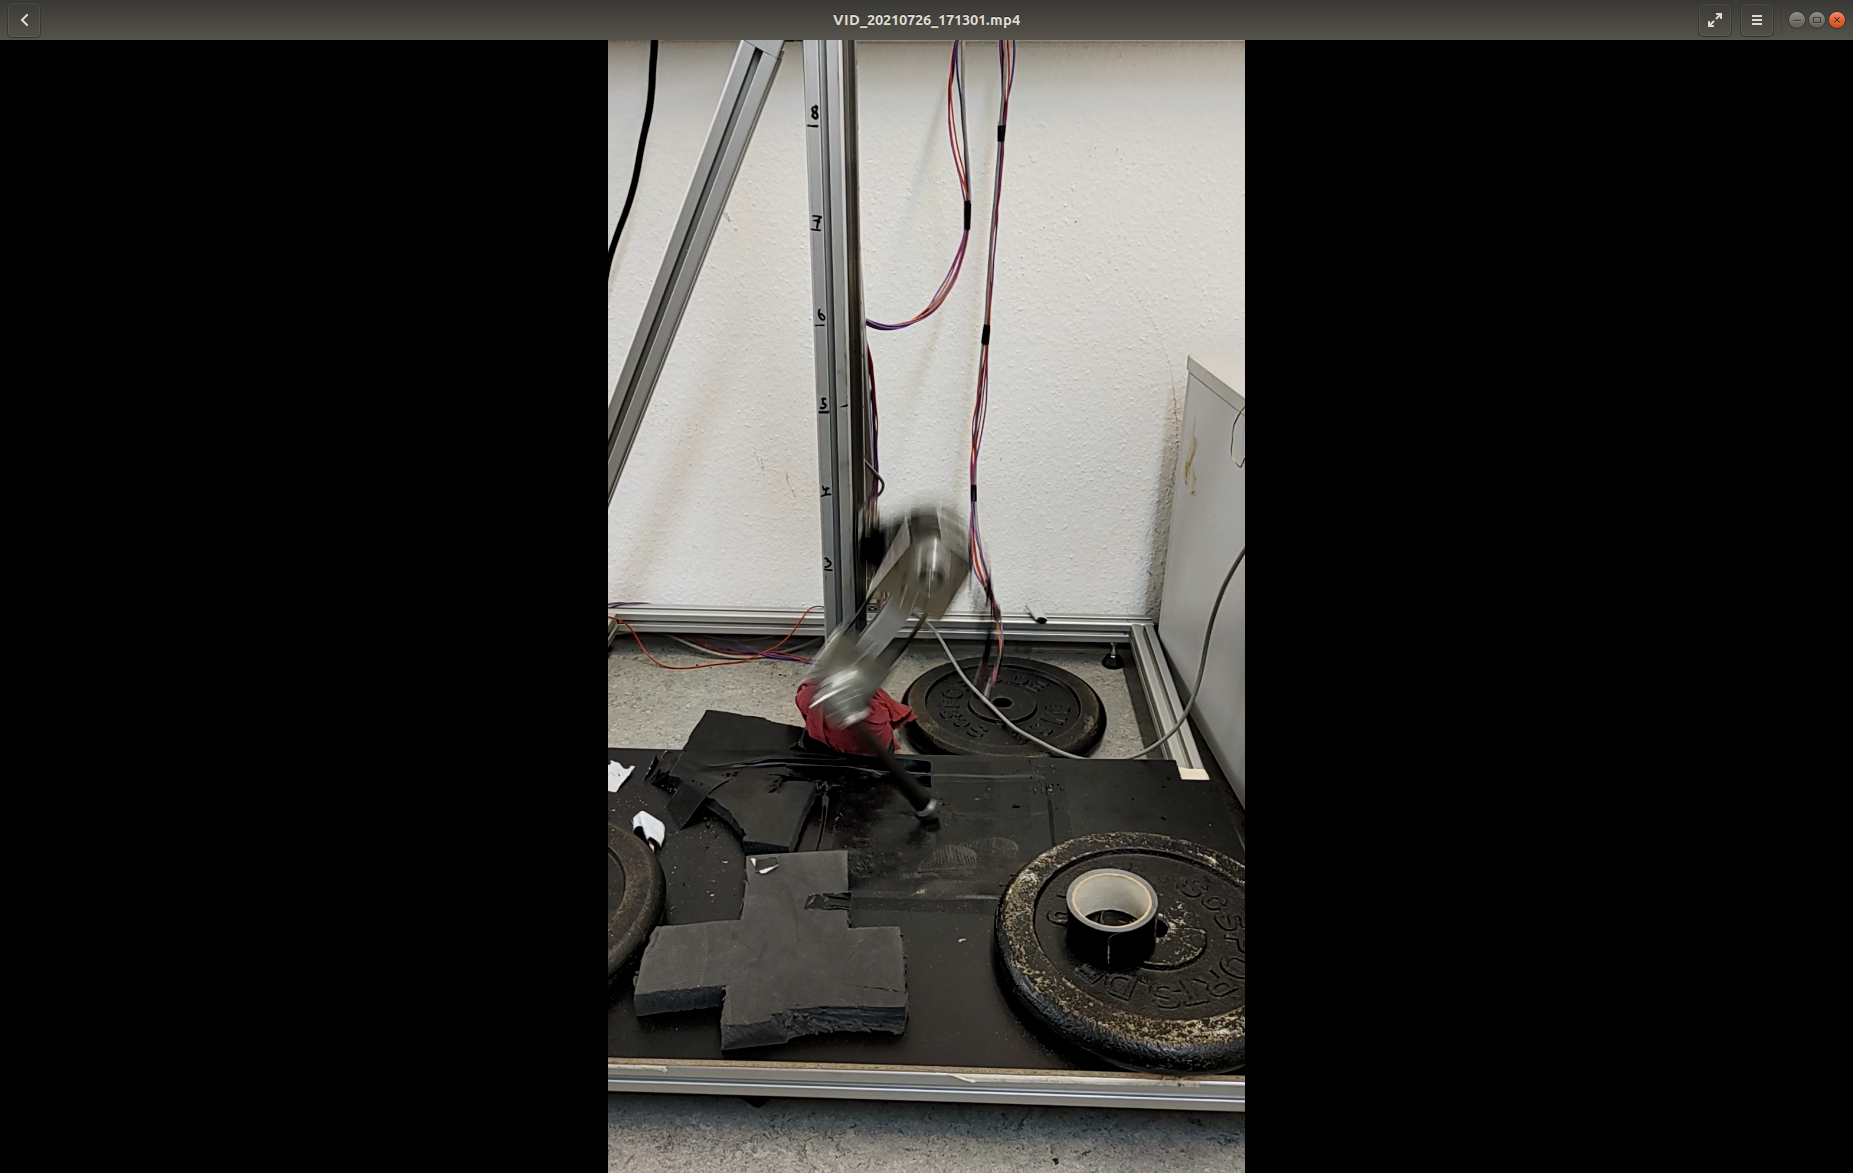
\includegraphics[width=\textwidth, trim={25cm 10cm 25cm 10cm}, clip]{figures/0.5m/p5m2.png}
    \end{subfigure}
    \begin{subfigure}{.24\textwidth}
    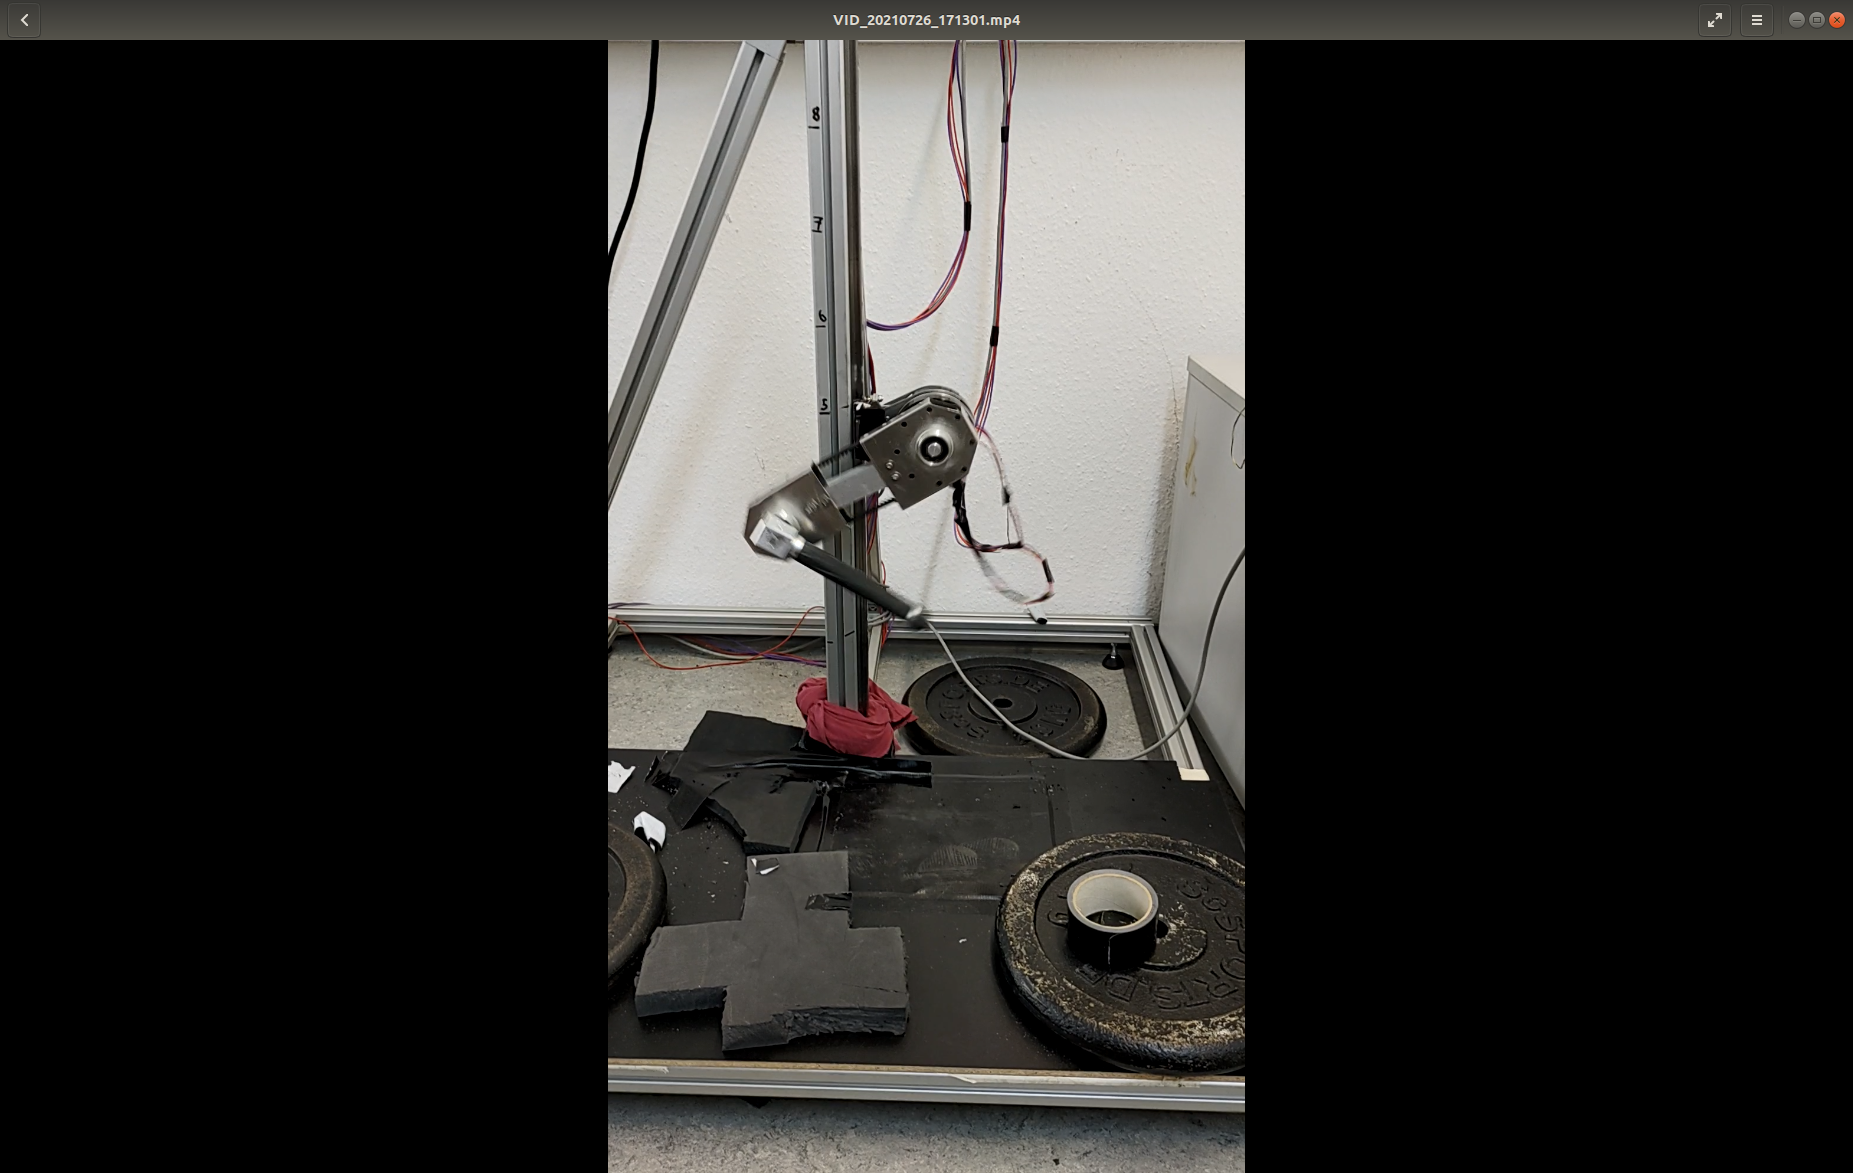
\includegraphics[width=\textwidth, trim={25cm 10cm 25cm 10cm}, clip]{figures/0.5m/p5m3.png}
    \end{subfigure}
    \begin{subfigure}{.24\textwidth}
    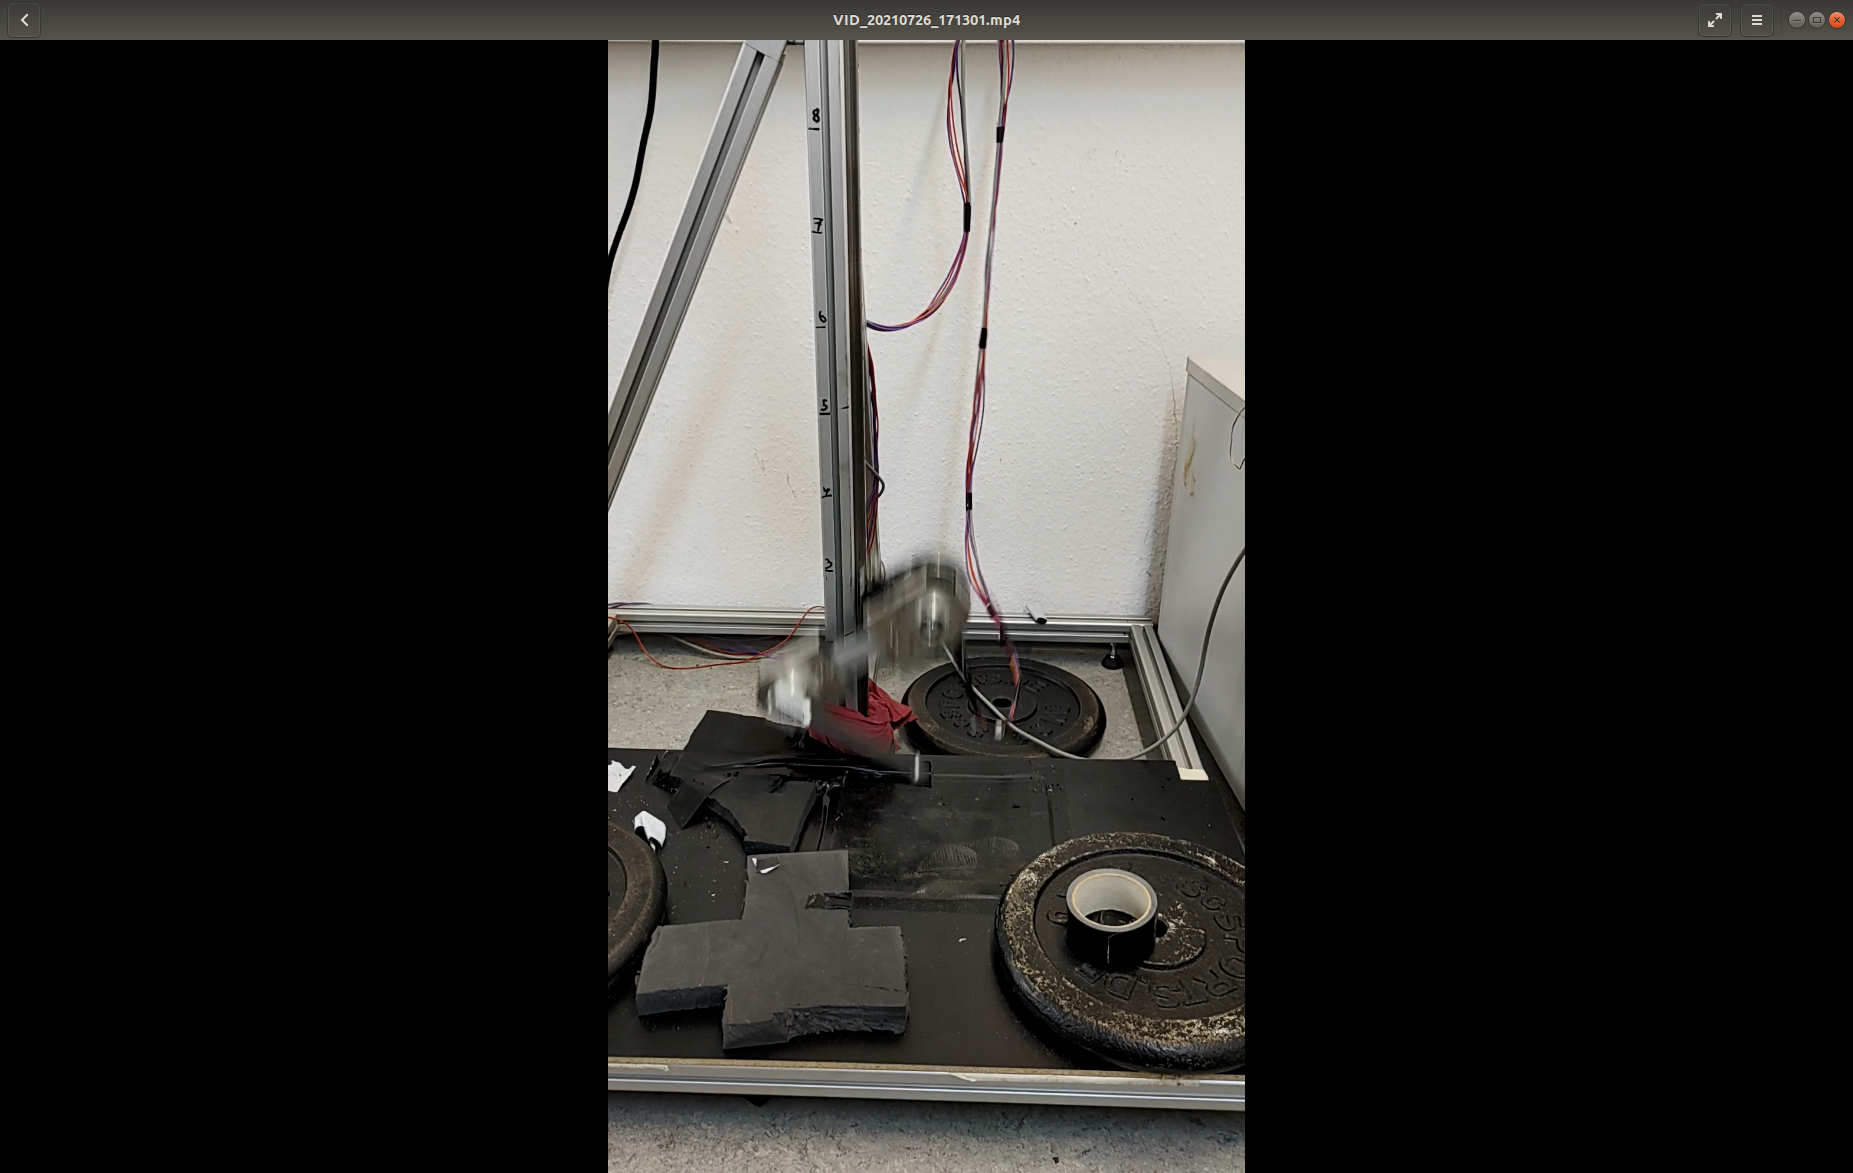
\includegraphics[width=\textwidth, trim={25cm 10cm 25cm 10cm}, clip]{figures/0.5m/p5m4.png}
    \end{subfigure}
    \caption{Jumping sequence for 0.5 m desired height}
    \label{fig:sequence5}
\end{figure}


\begin{figure}[htb!]
    \centering
    \begin{subfigure}{.24\textwidth}
    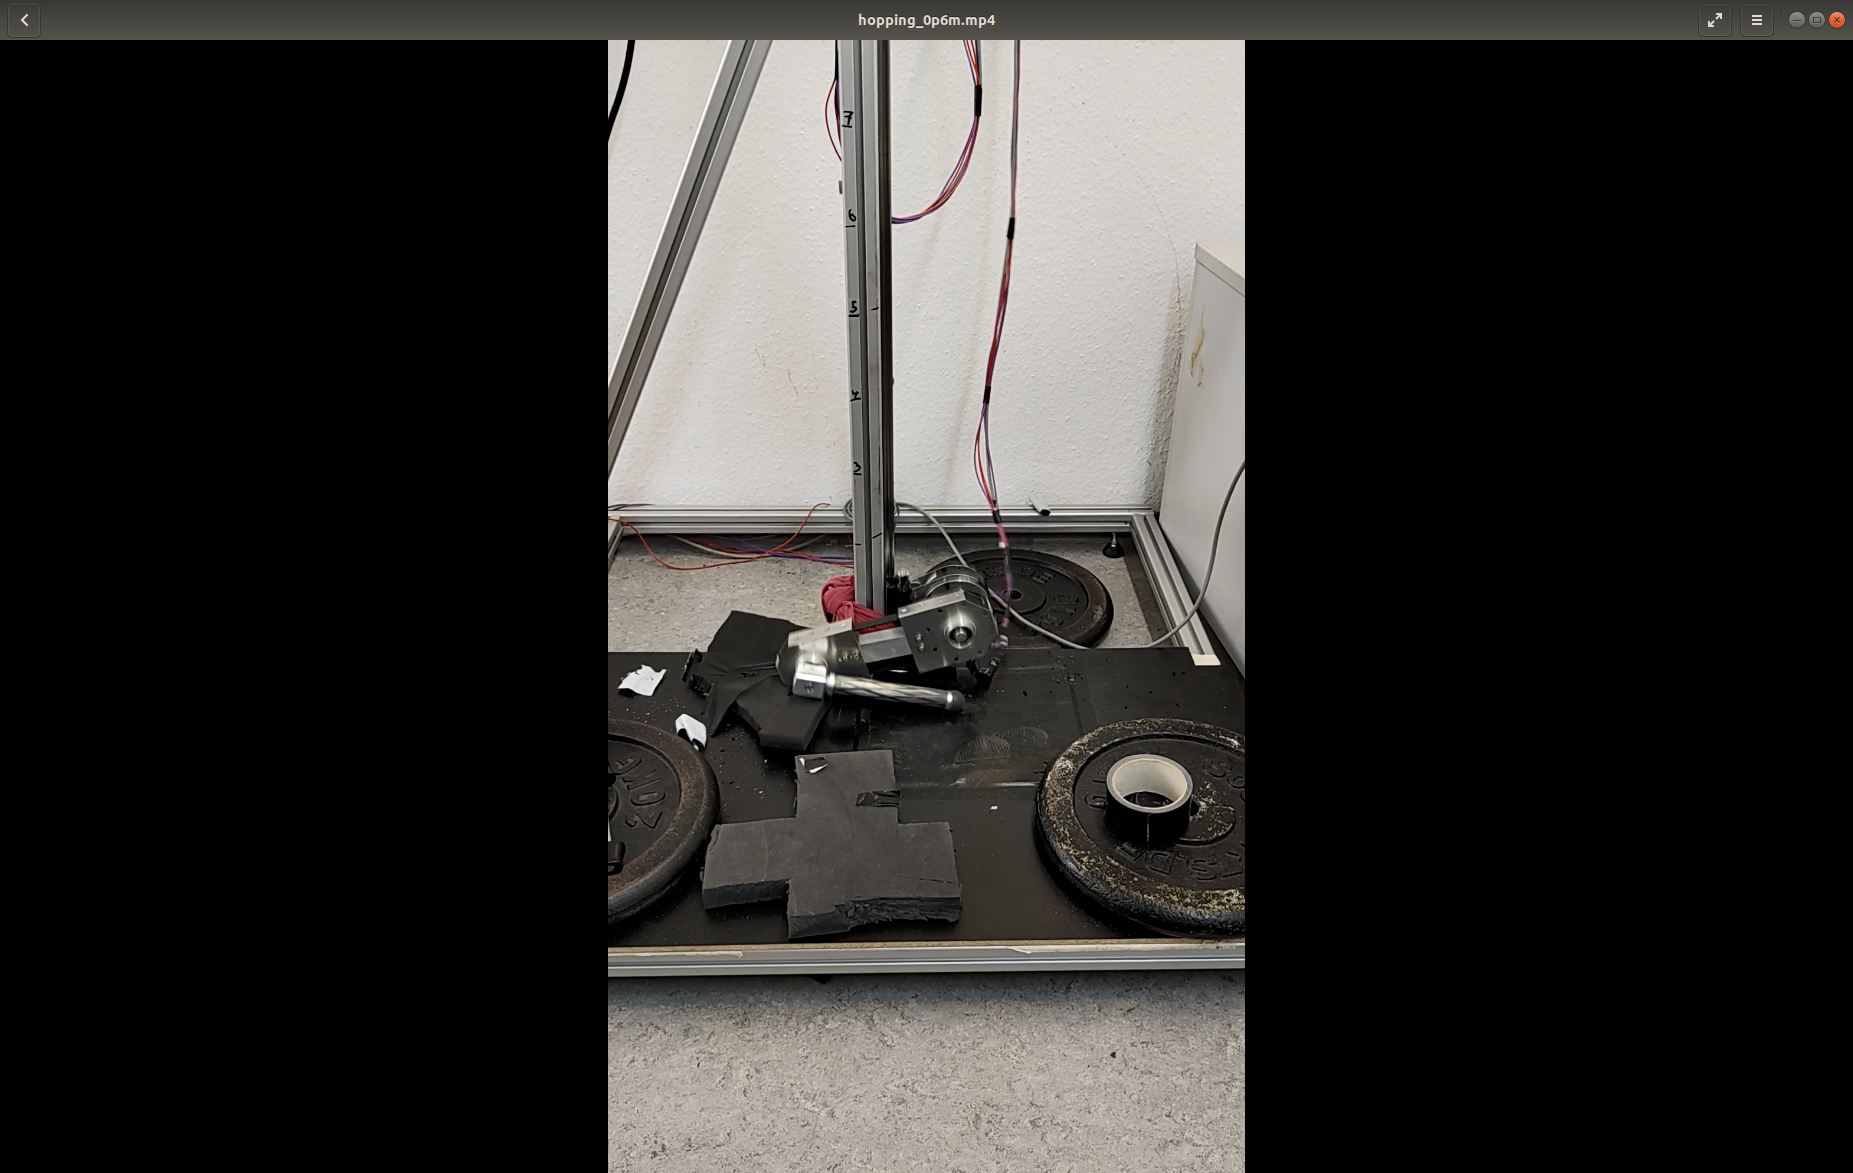
\includegraphics[width=\textwidth, trim={25cm 15cm 25cm 5cm}, clip]{figures/0.6m/p6m1.png}
    \end{subfigure}
    \begin{subfigure}{.24\textwidth}
    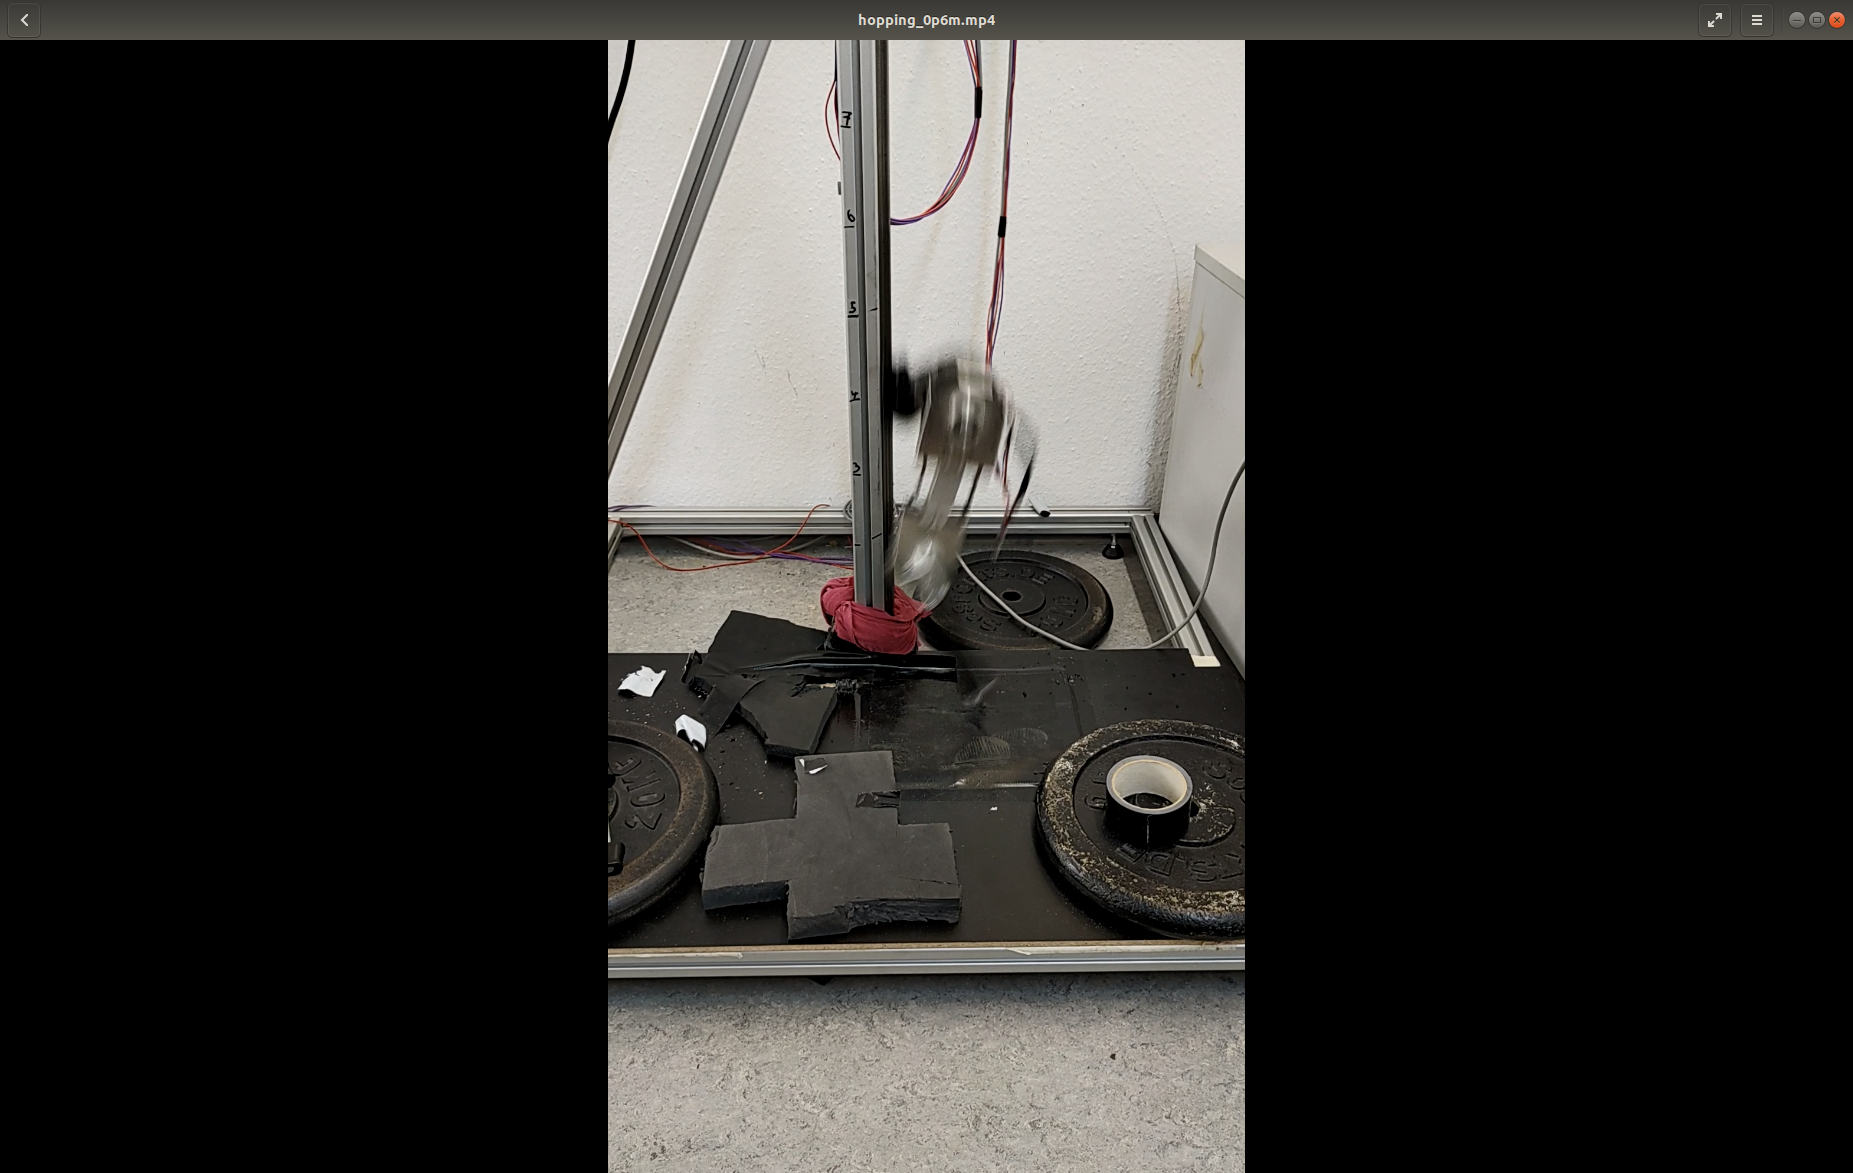
\includegraphics[width=\textwidth, trim={25cm 15cm 25cm 5cm}, clip]{figures/0.6m/p6m2.png}
    \end{subfigure}
    \begin{subfigure}{.24\textwidth}
    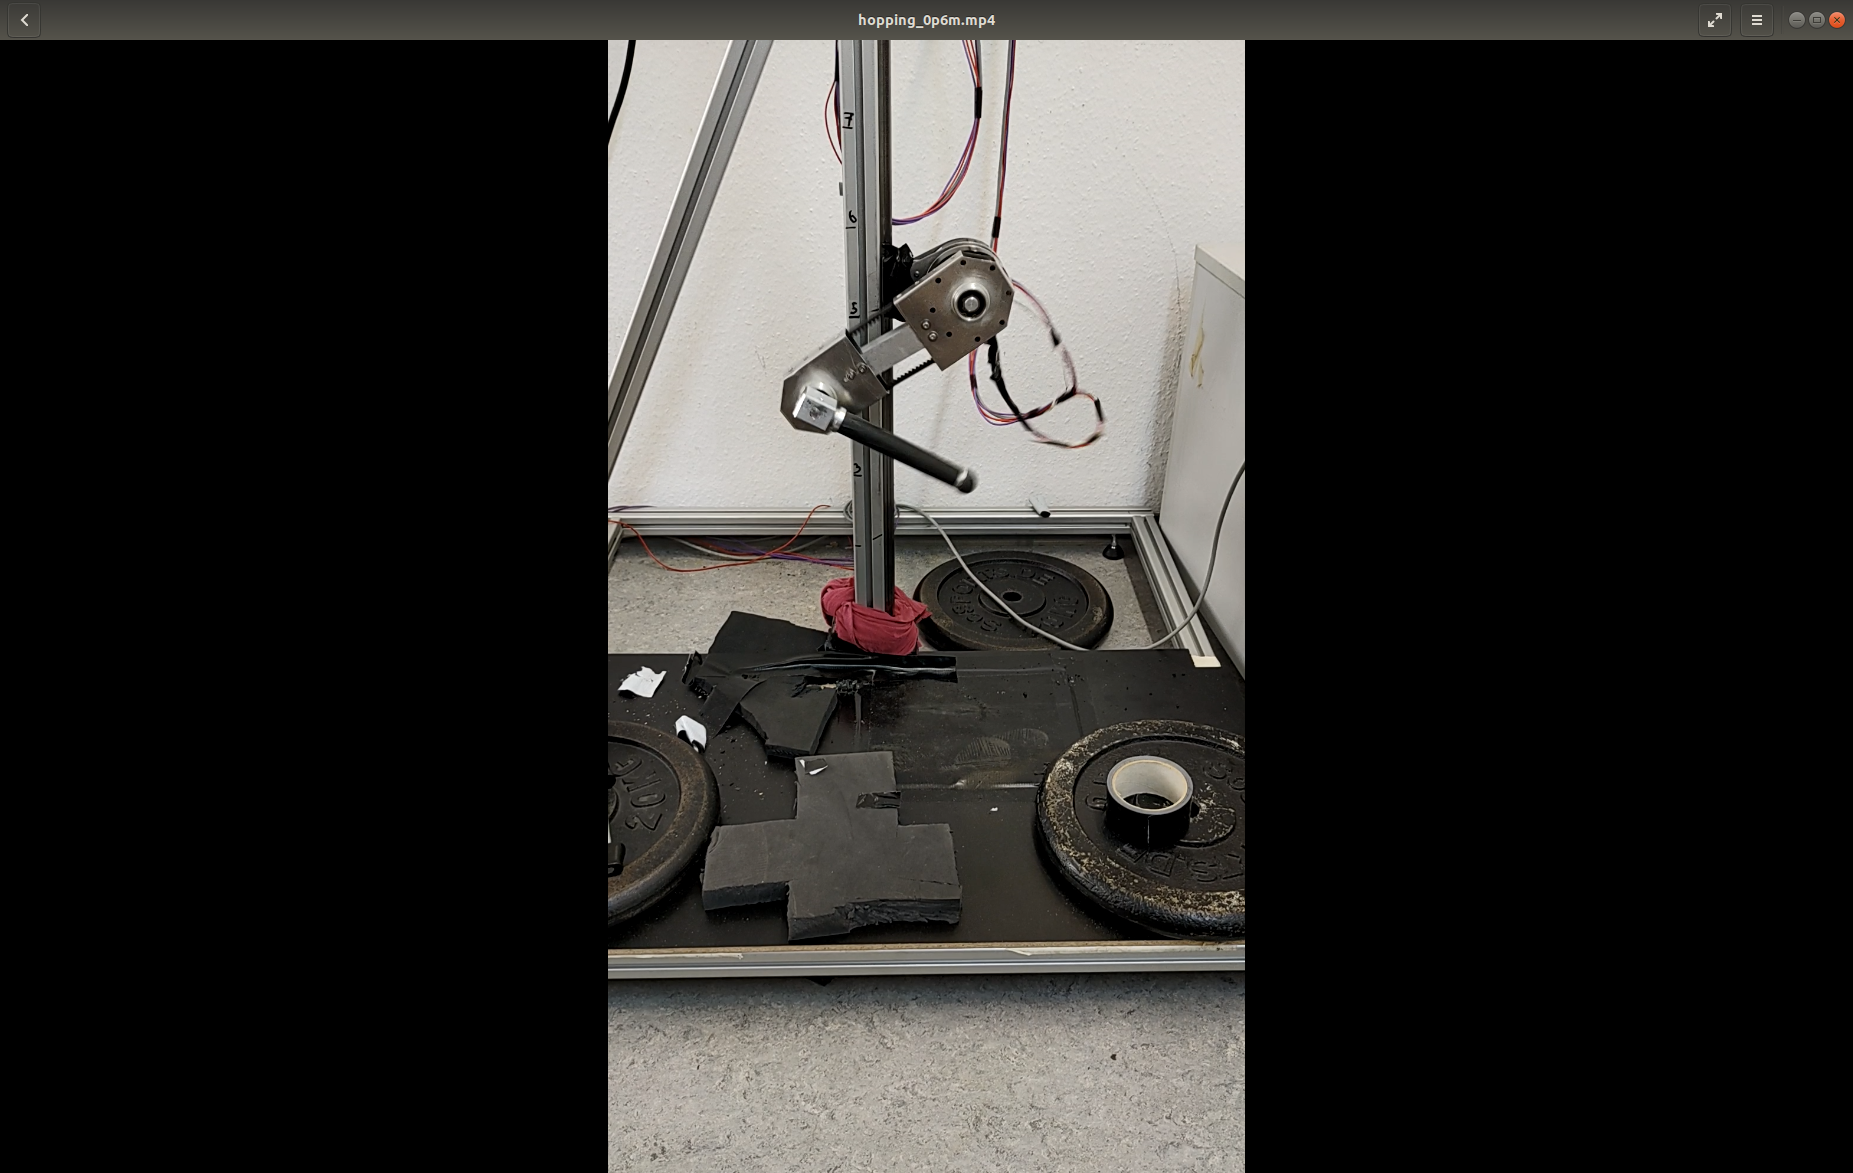
\includegraphics[width=\textwidth, trim={25cm 15cm 25cm 5cm}, clip]{figures/0.6m/p6m3.png}
    \end{subfigure}
    \begin{subfigure}{.24\textwidth}
    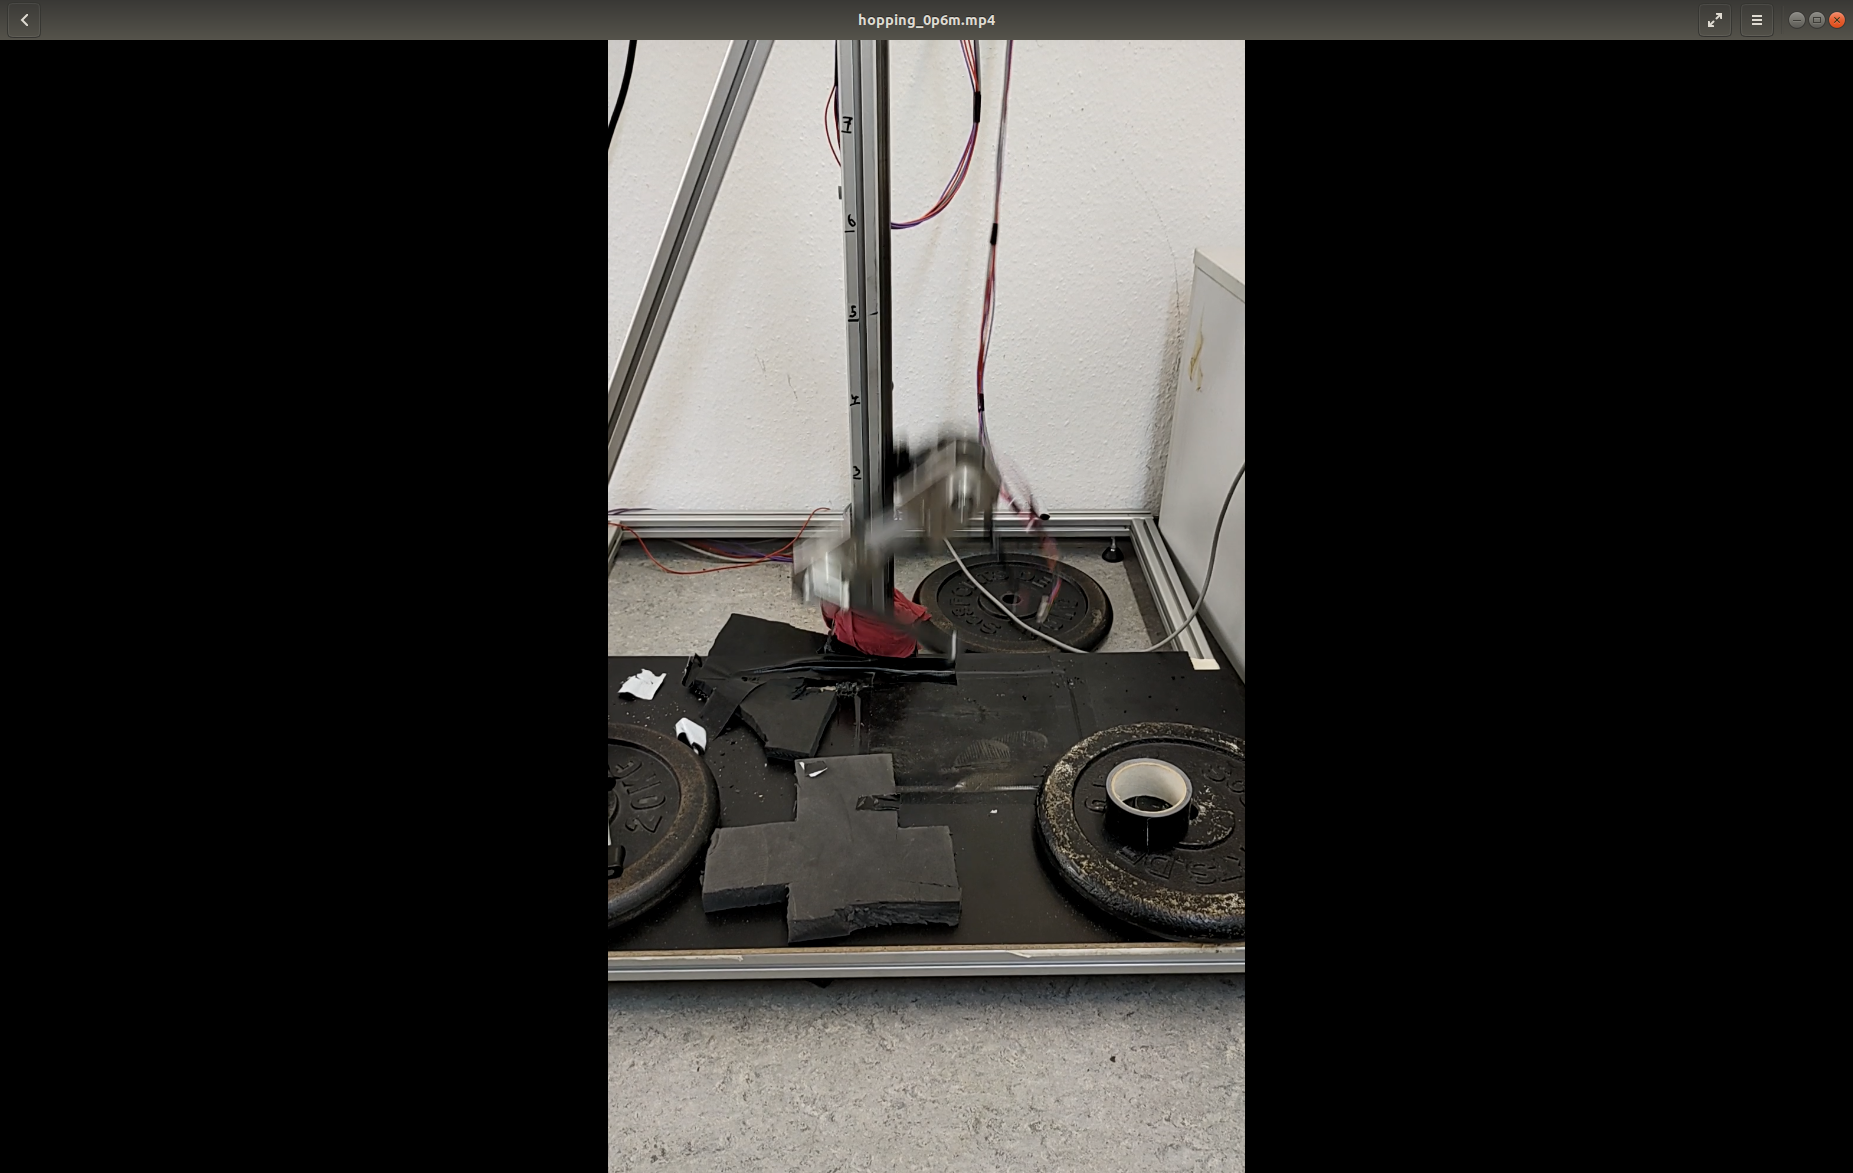
\includegraphics[width=\textwidth, trim={25cm 15cm 25cm 5cm}, clip]{figures/0.6m/p6m4.png}
    \end{subfigure}
    \caption{Jumping sequence for 0.6 m desired height}
    \label{fig:sequence6}
\end{figure}


\clearpage
\section{Backflip control}
In simulation, energy shaping control has been implemented inclusive backflip support. This backflip support adds
a trajectory to the current desired state and can follow arbitrary sequences of backflips, forward flips and normal jumps. In our simulations, we found that this backflip control works quite stable.
In \autoref{fig:simflip} you can see the sequence of an exemplary backflip in simulation.


\begin{figure}[htb!]
    \centering
    \begin{subfigure}{.16\textwidth}
    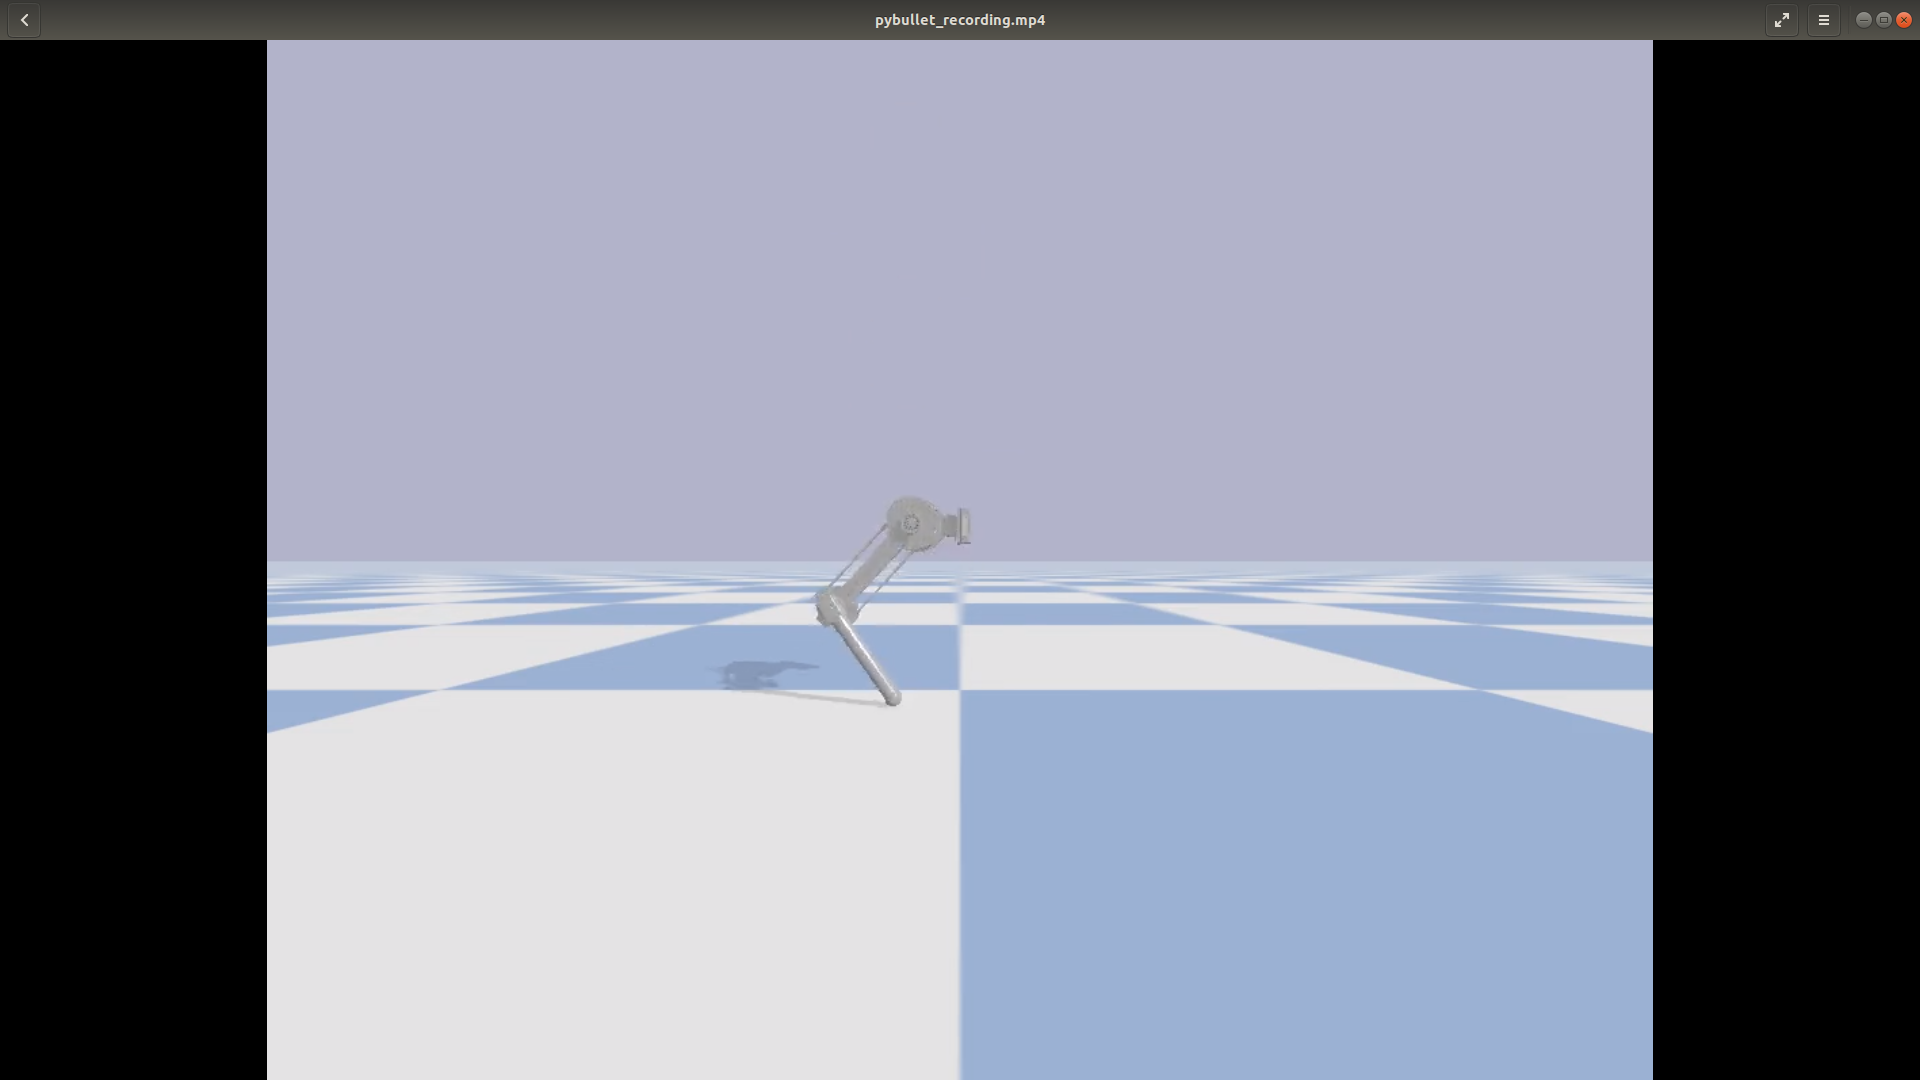
\includegraphics[width=\textwidth, trim={27cm 10cm 28cm 5cm}, clip]{figures/simBackflip/sb1.png}
    \end{subfigure}
    \begin{subfigure}{.16\textwidth}
    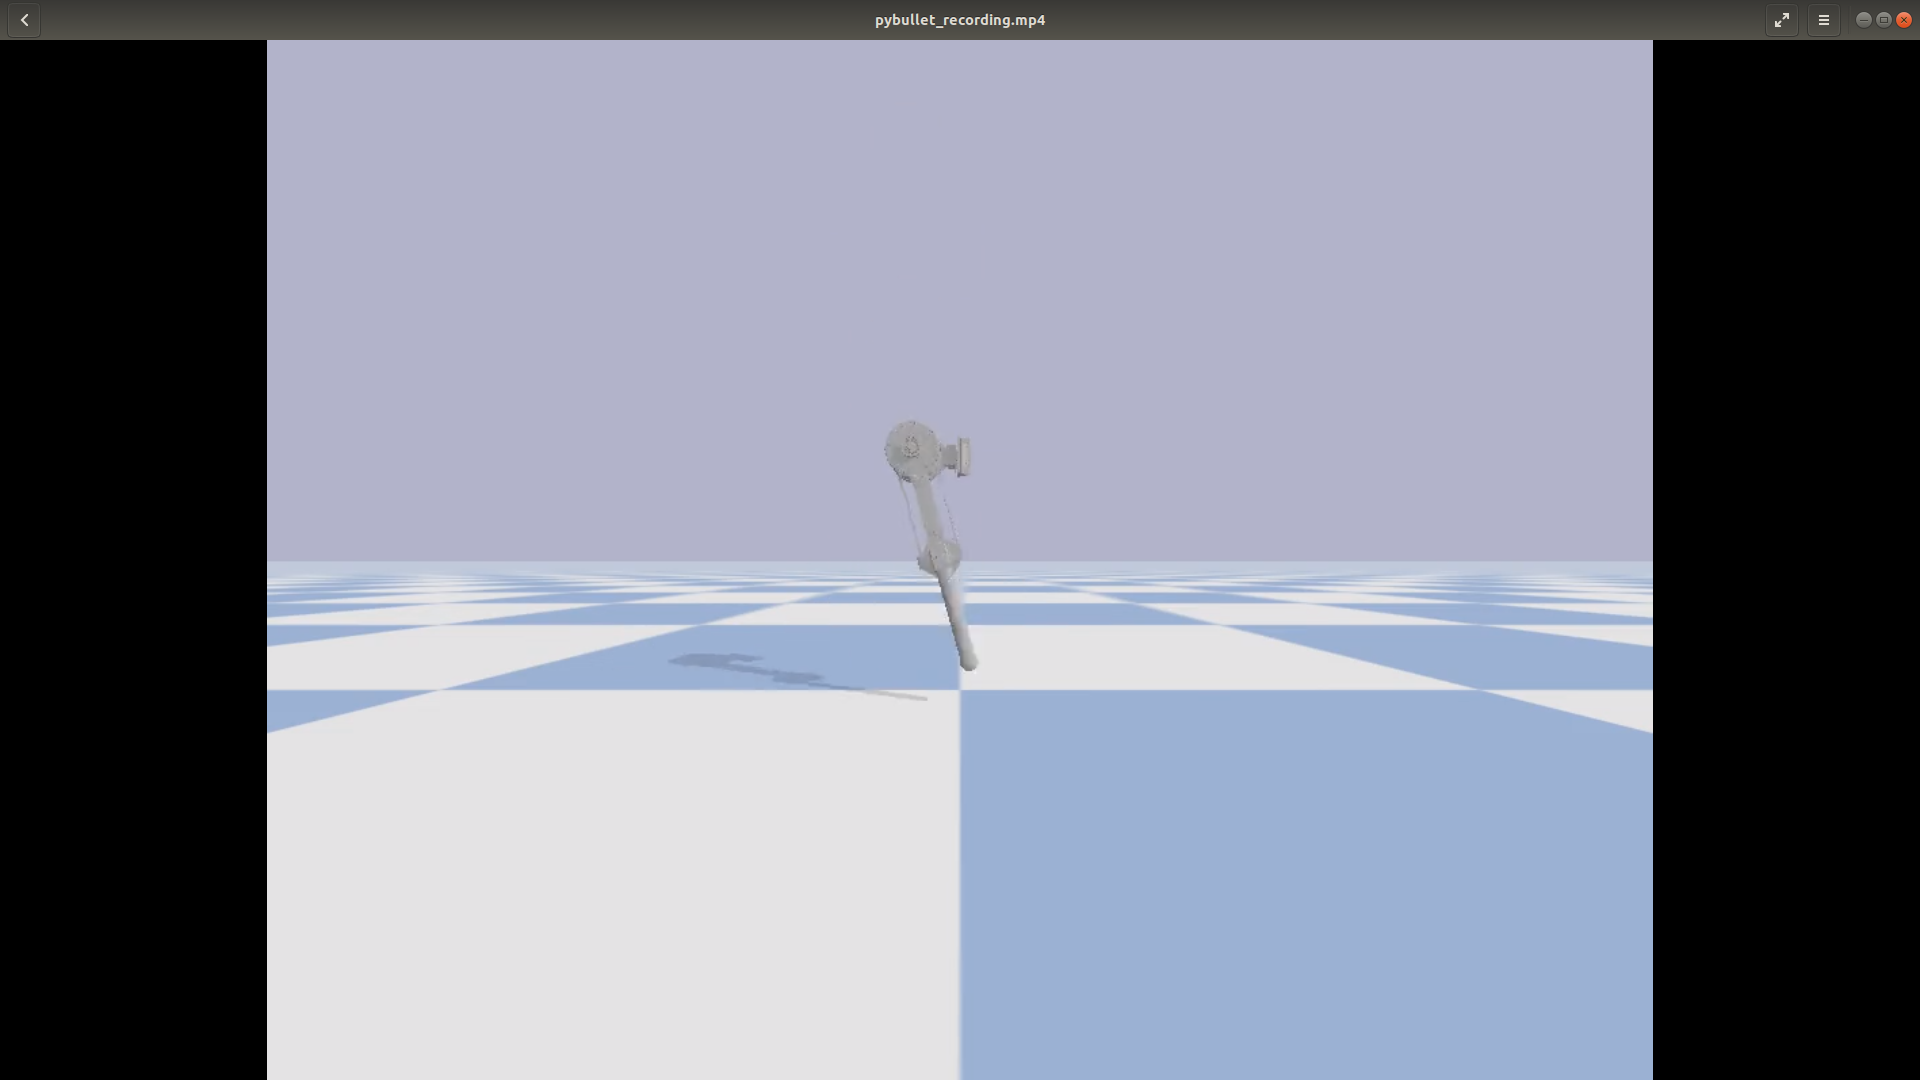
\includegraphics[width=\textwidth, trim={27cm 10cm 28cm 5cm}, clip]{figures/simBackflip/sb2.png}
    \end{subfigure}
    \begin{subfigure}{.16\textwidth}
    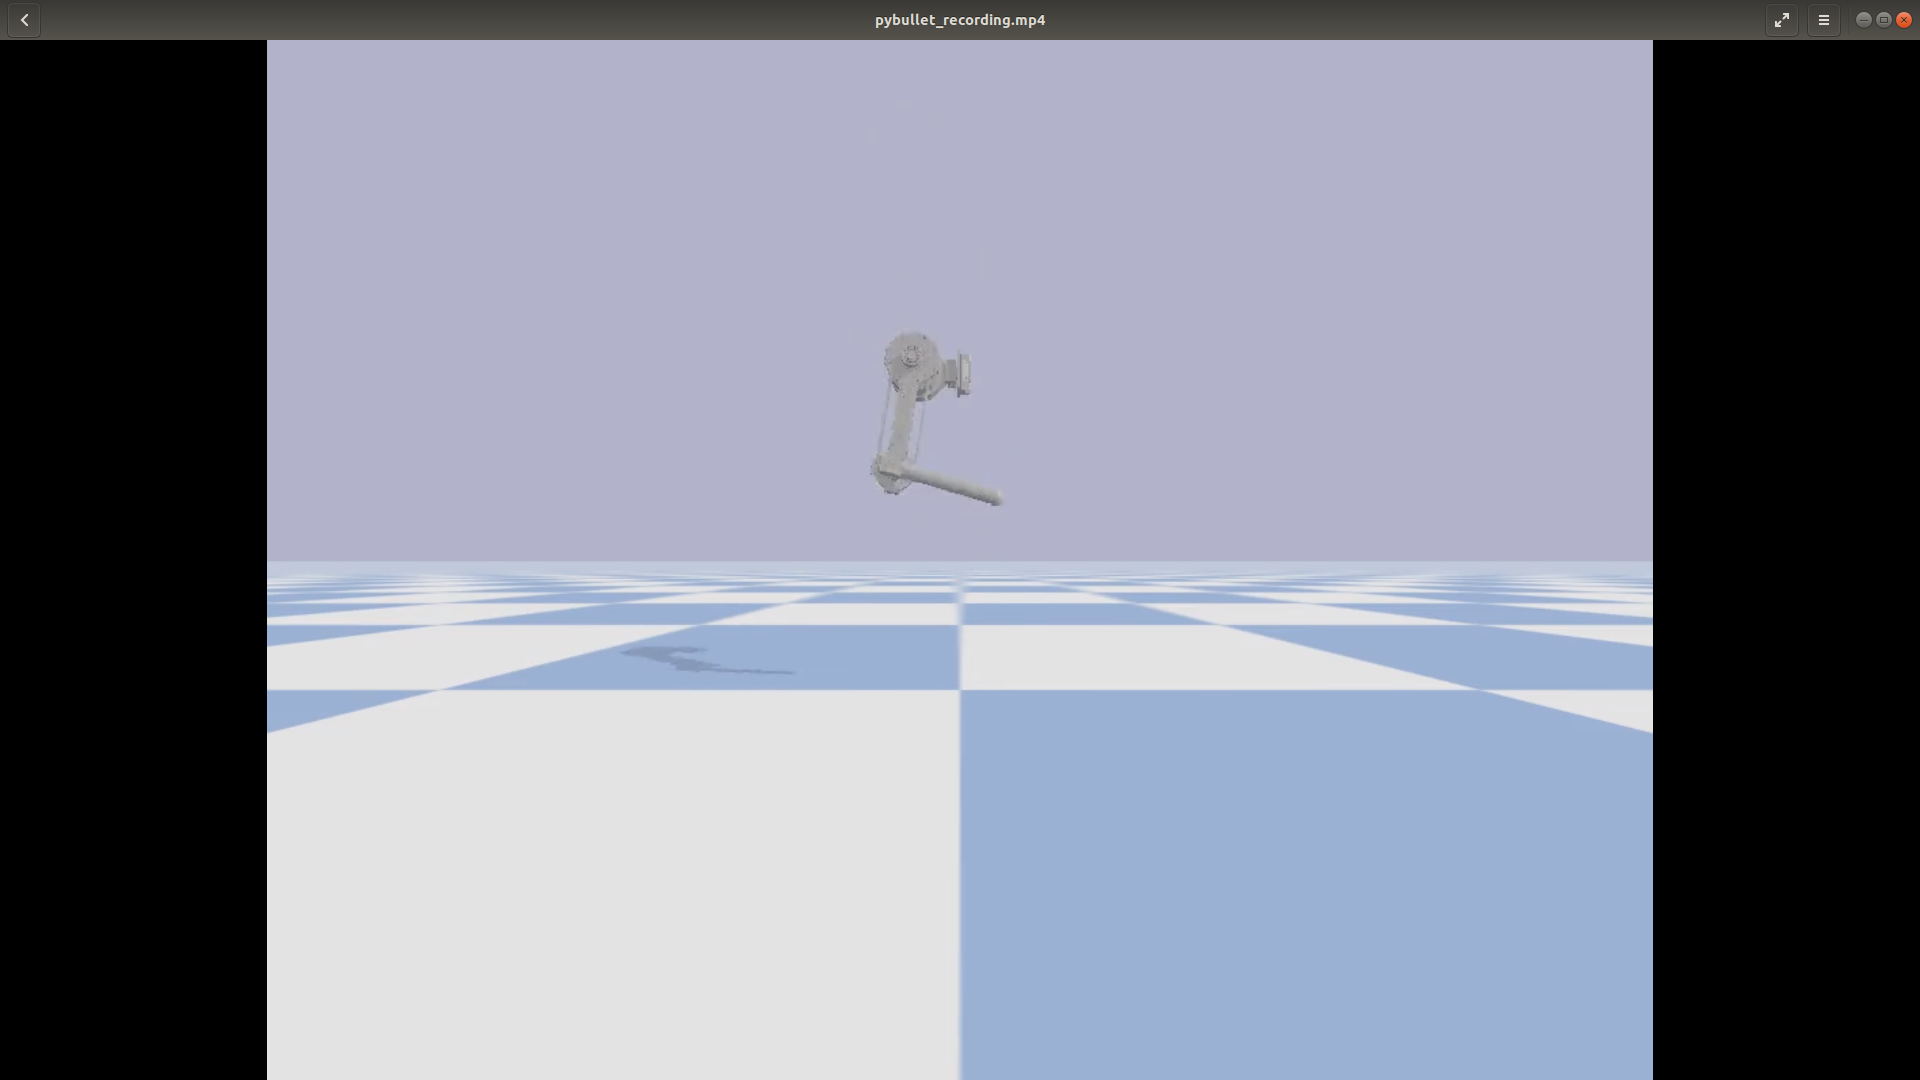
\includegraphics[width=\textwidth, trim={27cm 10cm 28cm 5cm}, clip]{figures/simBackflip/sb3.png}
    \end{subfigure}
    \begin{subfigure}{.16\textwidth}
    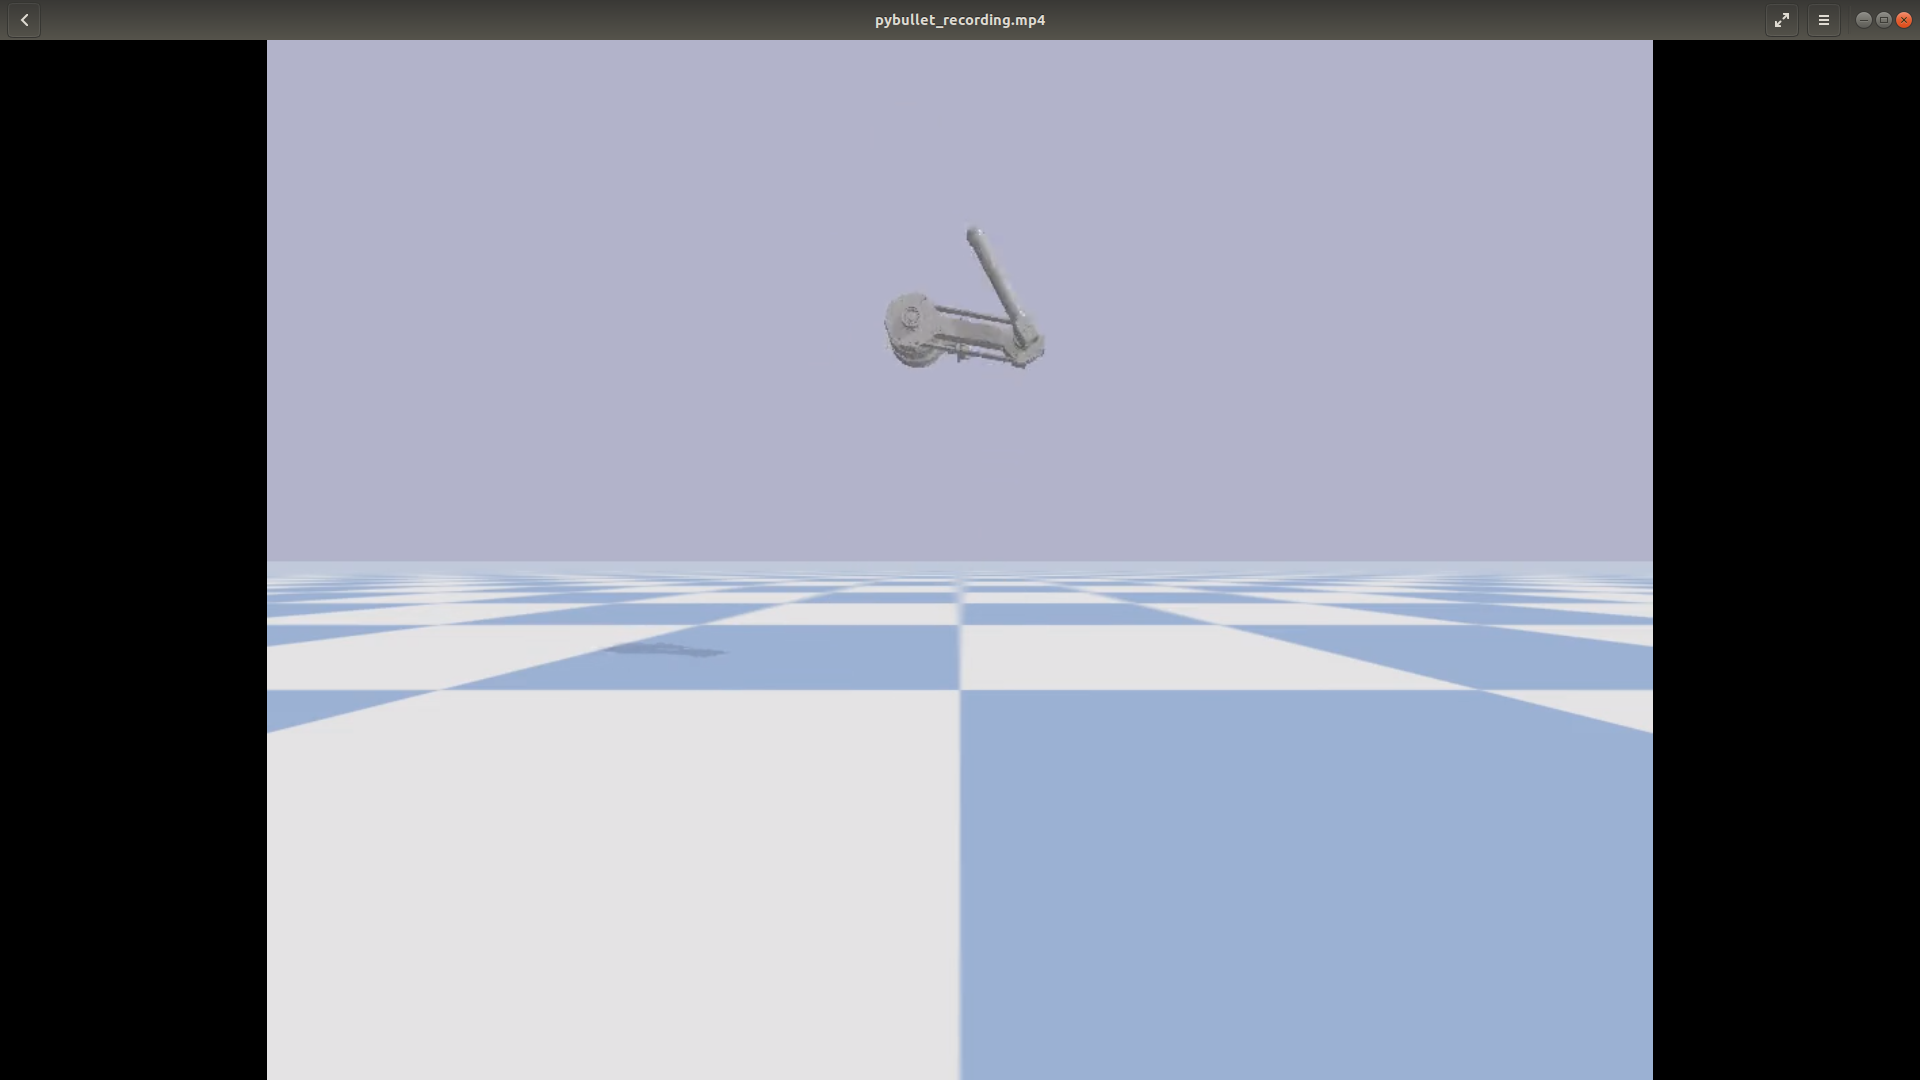
\includegraphics[width=\textwidth, trim={27cm 10cm 28cm 5cm}, clip]{figures/simBackflip/sb4.png}
    \end{subfigure}
    \begin{subfigure}{.16\textwidth}
    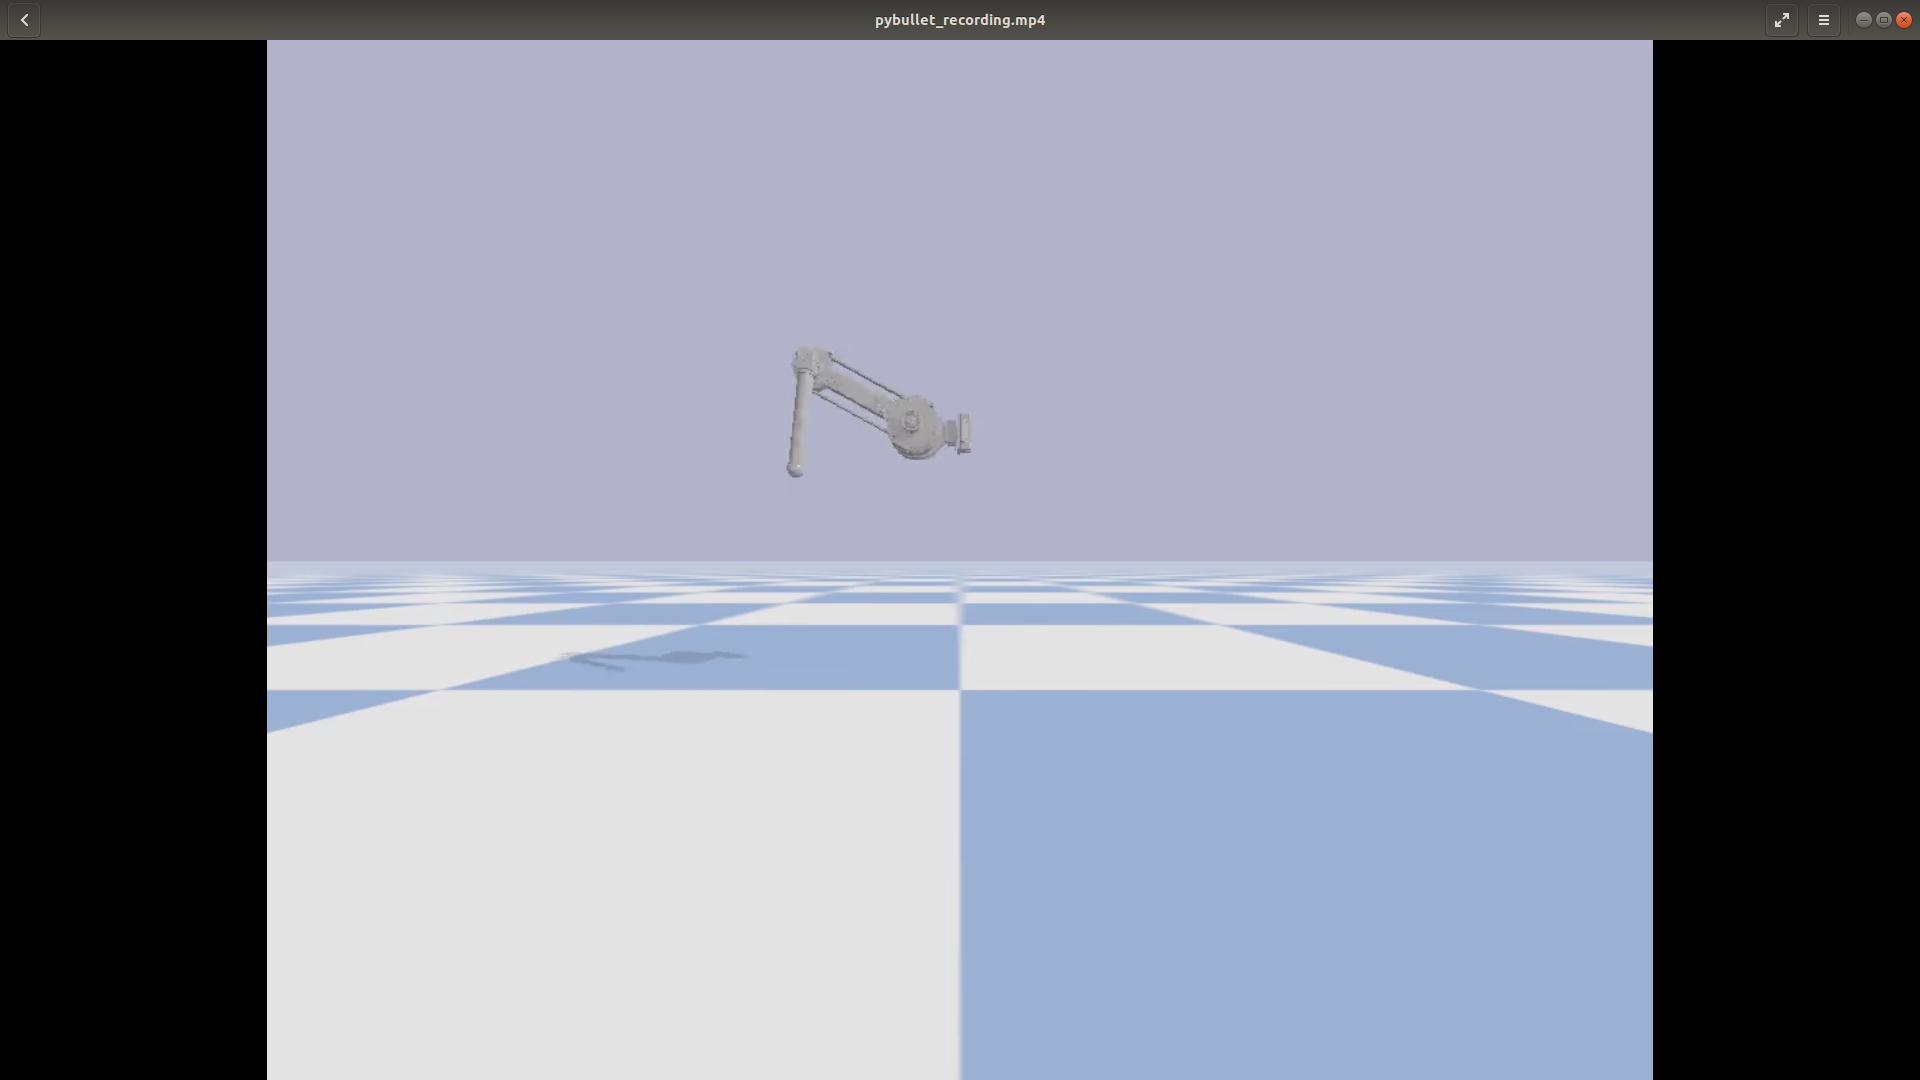
\includegraphics[width=\textwidth, trim={27cm 10cm 28cm 5cm}, clip]{figures/simBackflip/sb5.png}
    \end{subfigure}
    \begin{subfigure}{.16\textwidth}
    \includegraphics[width=\textwidth, trim={27cm 10cm 28cm 5cm}, clip]{figures/simBackflip/sb6.png}
    \end{subfigure}
    \caption{Simulated sequence of a backflip.}
    \label{fig:simflip}
\end{figure}


In the real system, we performed a backflip as well. Here we faced more issues due to the wiring, since the wires are likely to twist around the screws in the hopping leg. Hence, we lost the connection during our backflip. Nevertheless, we managed to do a full backflip. An image sequence of this is printed in \autoref{fig:flip}.
In future, it would be nice to try a sequence of forward- and backflips, as we have already implemented in simulation.

\begin{figure}[htb!]
    \centering
    \begin{subfigure}{.16\textwidth}
    \includegraphics[width=\textwidth, trim={27cm 10cm 27cm 5cm}, clip]{figures/backflip/b1.png}
    \end{subfigure}
    \begin{subfigure}{.16\textwidth}
    \includegraphics[width=\textwidth, trim={27cm 10cm 27cm 5cm}, clip]{figures/backflip/b2.png}
    \end{subfigure}
    \begin{subfigure}{.16\textwidth}
    \includegraphics[width=\textwidth, trim={27cm 10cm 27cm 5cm}, clip]{figures/backflip/b3.png}
    \end{subfigure}
    \begin{subfigure}{.16\textwidth}
    \includegraphics[width=\textwidth, trim={27cm 10cm 27cm 5cm}, clip]{figures/backflip/b4.png}
    \end{subfigure}
    \begin{subfigure}{.16\textwidth}
    \includegraphics[width=\textwidth, trim={27cm 10cm 27cm 5cm}, clip]{figures/backflip/b5.png}
    \end{subfigure}
    \begin{subfigure}{.16\textwidth}
    \includegraphics[width=\textwidth, trim={27cm 10cm 27cm 5cm}, clip]{figures/backflip/b6.png}
    \end{subfigure}
    \caption{Sequence of a backflip on the real system.}
    \label{fig:flip}
\end{figure}


\clearpage

\printbibliography[heading=bibintoc, title={Bibliography}]

\end{document}